\chapter{Resultados e Discuss�es}
\label{Resultados}

Neste cap�tulo s�o apresentados e discutidos os resultados obtidos a partir dos m�todos descritos na se��o \ref{metodosec}.

%%%%%%%%%%%%%%%%%%%%%%%%%%%%%%%%%%%%%%%%%%%%%%%%%%%%%%%%%%%%%%%%%%%%

\section{Estrutura mec�nica}
%\label{estmec}
%Para o projeto da parte mec�nica, em primeiro lugar foi concebida uma configura��o de sistema baseada tanto na literatura dispon�vel quanto em projetos de sistemas comerciais de produ��o de cerveja: um sistema de duas panelas an�logas � MT e ao BK, sendo que durante o processo de cozimento do mosto, o BK pudesse ser utilizado como HLT. Para atender a esta especifica��o, fez-se necess�rio o projeto de um sistema de recircula��o entre as duas panelas. Observa-se que esta proposta representa um h�brido entre o sistema de 3 panelas tradicional - que consiste de uma panela para mostura��o, uma para lavagem dos gr�os, ou \textit{sparging}, e uma para fervura; e o sistema popularizado pela Braumeister, composto de 1 panela, com recircula��o. Esta abordagem permitiu a economia financeira e simplifica��o mec�nica do sistema de tr�s panelas com o benef�cio do \textit{sparging} inexistente no sistema de uma panela.

\subsection{Funcionamento da estrutura}

Na figura \ref{esboco} � apresentada uma representa��o esquem�tica da parte funcional.

\begin{figure}[H]
	\centering
	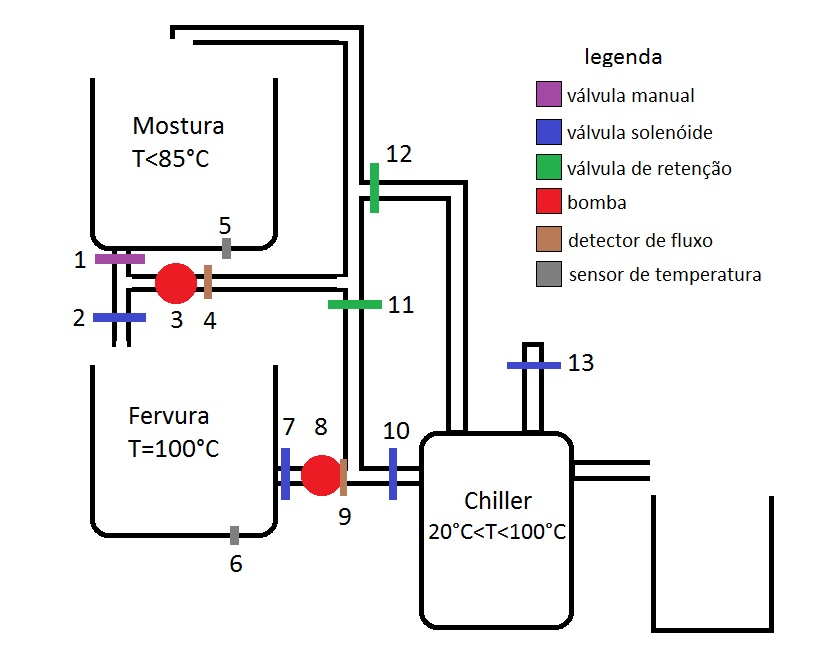
\includegraphics[scale=0.55]{./Resources/esb_mec.jpg}
	\captionsetup{justification=centering}
	\caption[Representa��o esquem�tica da estrutura mec�nica]{Representa��o esquem�tica da estrutura mec�nica}
	\label{esboco}
\end{figure}

Na panela superior ou MT, rotulada como \textit{Mostura}, os gr�os s�o adicionados ap�s o aquecimento inicial da �gua:

\begin{itemize}
	\item A v�lvula 1 � uma v�lvula manual do tipo esfera, com passagem plena. Durante a opera��o do equipamento ela deve ficar sempre aberta, portanto seu uso � realizado somente em caso de emerg�ncias.
	\item Ap�s a adi��o dos gr�os, a bomba 3 � ligada para que o l�quido da panela seja recirculado. As v�lvulas de reten��o 11 e 12 n�o permitem que o l�quido passe por elas, portanto h� somente um caminho poss�vel para este, que � ascender pela tubula��o at� entrar novamente na MT. Note-se que n�o h� v�lvula automatizada na sa�da da MT, uma vez que o mosto fica em recircula��o constante ao longo do processo de cozimento.
	\item Ap�s a mostura a bomba 3 � desligada e a v�lvula solen�ide 2 � aberta, escoando o l�quido para a panela de fervura BK. Simult�neamente, a v�lvula solen�ide 7 e a bomba 8 s�o ativadas, fazendo com que a �gua de lavagem presente na BK/HLT flua pela tubula��o at� a MT, iniciando o processo de \textit{sparging}. Durante um tempo predefinido, o mosto e a �gua de lavagem recirculam pelas duas panelas e se misturam.
	\item Durante a fervura, as v�lvulas 2 e 7 s�o fechadas. Neste per�odo, os gr�os drenados que est�o na MT devem ser retirados manualmente, j� que ela ser� usada posteriormente para armazenamento da �gua de esfriamento do mosto --- �gua usada para limpeza do sistema e que reduz a produ��o de efluentes do mesmo.
	\item Ap�s a fervura, as v�lvulas solen�ides 7 e 10 s�o ativadas, permitindo o escoamento do l�quido para o trocador de calor. Simult�neamente a v�lvula solen�ide 13 � aberta e �gua fria circula em contra-fluxo para resfriar o mosto. Esta �gua sai quente do trocador de calor e passa pela v�lvula de reten��o 12, preenchendo a parte superior da tubula��o e sendo armazenada na MT para posterior limpeza do sistema.
	\item O mosto que sai resfriado do \textit{chiller} cai no balde de fermenta��o. Neste processo o l�quido entra em contato com o ar, o que � n�o somente desej�vel como essencial para o sucesso da fermenta��o, portanto esta � a �ltima parte automatizada que tem rela��o com a cerveja. Uma solu��o futura e que permite automa��o desta transi��o � o uso de um aerador em conjunto com um tanque de fermenta��o selado.
	\item Por fim, a �gua armazenada na MT � aquecida e recirculada pelo sistema, promovendo uma limpeza preliminar deste.
\end{itemize}

\pagebreak

Para o bom funcionamento do sistema proposto, algumas condi��es devem ser atendidas:

\begin{itemize}
	\item Se o volume total de l�quido nas duas panelas ao final da mostura exceder o volume da BK, ela transbordar�. Por este motivo � importante que exista um sistema de detec��o de transbordo. Ainda assim, deve-se requisitar que o usu�rio do sistema calcule corretamente as propor��es da receita, pois mesmo que seja aplicado um sistema autom�tico anti-transbordo, ocorrer� perda de insumos devido ao ac�mulo de mosto inutiliz�vel na MT em caso de erro.
	\item S�o necess�rios filtros de material particulado na sa�da das panelas para o bom funcionamento das v�lvulas e bombas \cite{danfoss_solenoid}.
	\item Os dispositivos mec�nicos (v�lvulas, bombas, tubula��o, dentre outros) e eletr�nicos (sensores e atuadores) em contato com o sistema mec�nico devem ser apropriados �s altas temperaturas impostas pela natureza do processo \cite{danfoss_solenoid, jefferson_solenoid}.
	\item As panelas, tendo como refer�ncia seu fundo, n�o devem ser alinhadas conc�ntricas, j� que isto torna a adi��o de l�pulos e o processo de manuten��o do equipamento desajeitados.
	\item A automa��o da t�cnica de \textit{whirlpool} n�o � contemplada nesta configura��o de sistema. Se o usu�rio a considera necess�ria, ele deve se encarregar de execut�-la manualmente.
	\item A �nica v�lvula com press�o suficiente para ser servo-operada � a 13, assumindo-se que a press�o incidente sobre ela seja maior do que 0,5bar, portanto as outras devem ser de opera��o direta \cite{danfoss_solenoid, jefferson_solenoid}.
	\item A limpeza automatizada, ou CIP, n�o � contemplada em sua totalidade nesta configura��o do sistema, devido � alta complexidade \cite{cip_pres}, conforme indica a figura \ref{cip_system}, e ao custo de implementa��o proibitivo para o presente trabalho. N�o obstante, � recomendado ao usu�rio do sistema que fa�a a limpeza do mesmo t�o r�pido quanto poss�vel ap�s o final da produ��o.
\end{itemize}

\begin{figure}[H]
	\centering
	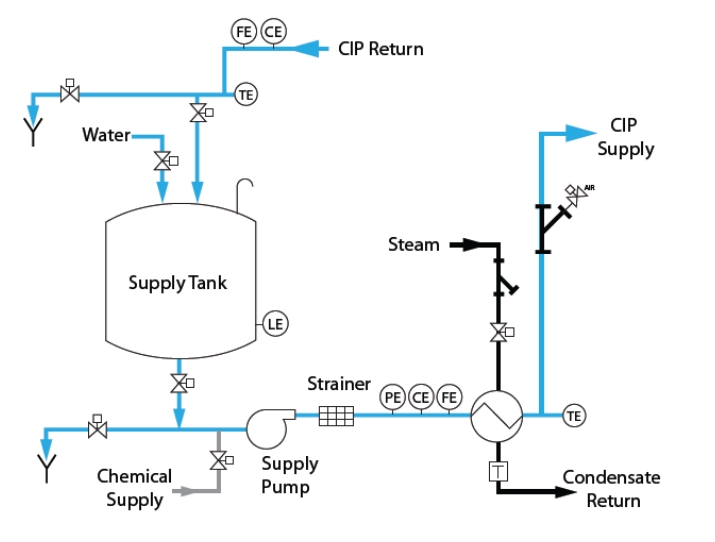
\includegraphics[scale=0.55]{./Resources/cip_example.jpg}
	\captionsetup{justification=centering}
	\caption[Sistema CIP b�sico]{Sistema CIP b�sico. \\Fonte: ROSE e MONTGOMERY (2010)}
	\label{cip_system}
\end{figure}

\subsection{Dimensionamento da parte funcional} 

Com a filosofia de opera��o do sistema mec�nico definida, foi poss�vel realizar o dimensionamento deste sistema. A primeira considera��o a ser feita � que os materiais e m�todos aqui empregados n�o seguem nenhuma norma que permita o uso deste equipamento para fabrica��o de cerveja visando sua comercializa��o --- tal escolha foi feita em fun��o do alto custo de um sistema completamente dentro das normas e tamb�m pelo fato de este ser um trabalho cujo foco � a automa��o e o acesso remoto do sistema, e n�o a comercializa��o de cerveja.

N�o obstante, o material da tubula��o escolhido foi o a�o inoxid�vel AISI304. J� que o volume de l�quido a ser trabalhado � pequeno, menor do que 40 litros, e a press�o de trabalho n�o � maior do que a press�o das bombas escolhidas posteriormente, foi decidido o uso de tubula��o de di�metro de 1/2" (21,34mm de di�metro externo) e espessura da parede no padr�o Schedule 40 (2,77mm de espessura). Embora esta espessura seja superdimensionada para a presente aplica��o, o mec�nico respons�vel pela montagem do sistema a requisitou para que fosse poss�vel fazer rosca sem danificar a integridade dos tubos. As conex�es, seguindo a escolha dos tubos, tamb�m foram de a�o inoxid�vel de 1/2".

As liga��es entre tubos, conex�es e outros componentes do sistema s�o liga��es rosqueadas. Este � um meio de liga��o antigo, por�m de baixo custo, f�cil execu��o e usualmente empregadas em tubula��es de di�metro nominal pequeno, menor do que 4" \cite{ifba}. Para veda��o foi escolhido o Teflon, uma vez que � um material de baixo custo e alta disponibilidade e o padr�o de rosca adotado neste projeto � o BSP, baseado na norma ISO. Cabe salientar que, embora as liga��es rosqueadas sejam permitidas sob certas circunst�ncias na pr�tica, elas s�o relegadas a instala��es de baixa responsabilidade \cite{ifba}.

As panelas foram escolhidas no material de alum�nio, em fun��o do custo proibitivo do a�o inoxid�vel. S�o caldeir�es padr�o utilizados no ramo de hotelaria e restaurantes e dispon�veis em v�rios volumes. As duas panelas utilizadas neste trabalho tem capacidade para 32 litros e di�metro do fundo de 36cm, portanto sua especifica��o no mercado � \textit{caldeir�o de alum�nio n. 36}. Tal volume, 60\% superior ao da produ��o m�xima aconselhada para este sistema, � necess�rio devido ao volume dos gr�os, � quantidade da �gua de lavagem e �s perdas por evapora��o que exigem uso de um volume de �gua inicial superior ao nominal.

O par�metro inicial escolhido para sele��o das v�lvulas solen�ide foi a temperatura m�xima de opera��o, cuja fonte de dados de opera��o � fornecida pelos fabricantes. Em seguida, foi escolhida uma veda��o adequada: os dois tipos mais comums de veda��o com suporte a temperatura de pelo menos 100\si{\degree}C s�o o EPDM e FKM (etileno-propileno-dieno e fluoreto de vinilideno, respectivamente) \cite{danfoss_solenoid}. Estes materiais possuem uma tabela de compatibilidade de fluidos cuja classifica��o pode ser satisfat�ria, boa, duvidosa, insatisfat�ria e desconhecida --- tanto para cerveja quanto para o mosto, ambas as veda��es s�o classificadas como satisfat�rias, embora para �gua a classifica��o do FKM seja somente boa \cite{epdm_fkm}. Por fim, um par�metro que foi verificado antes da escolha final das v�lvulas � a posi��o de opera��o, que varia conforme os modelos do fabricante \cite{danfoss_solenoid}. Com base nos par�metros supracitados, foi decidido usar:

\begin{itemize}
	\item V�lvula solen�ide 1/2" 12V pl�stico uso geral para �gua de resfriamento do trocador de calor.
	\item V�lvula solen�ide Danfoss 1/2" EV210BD 032U3620 para demais v�lvulas.
	\item Solen�ide Danfoss 15W 12VDC 042N7550 para acionamento das v�lvulas Danfoss.
\end{itemize}

Informa��es t�cnicas sobre a v�lvula EV210BD 032U3620 est�o no anexo \ref{Anexo3} e sobre a bobina 042N7550 no anexo \ref{Anexo4}.

As bombas de recircula��o foram escolhidas com base na temperatura de opera��o e grau aliment�cio. Posteriormente, tanto a vaz�o quanto a perda de carga do sistema foram estimadas para verificar se a bomba escolhida era adequada: o modelo Topsflo B08H-12-1006 tem capacidade m�xima de vaz�o de 10l/min e carga expressa em coluna de �gua de 6m. Como a capacidade m�xima do sistema � de 20l e idealmente a temperatura deve subir � taxa de 1\si{\degree}C/min, al�m de que a altura do sistema � menor do que 2m e as perdas de carga n�o decorrentes da gravidade foram consideradas desprez�veis para este caso, foi decidido que a bomba escolhida � adequada ao projeto. No anexo \ref{Anexo5} encontra-se a folha de dados t�cnicos do dispositivo.

Quanto �s conex�es, a figura \ref{conexoes_rascunho} apresenta um diagrama conceitual do sistema, contendo as pe�as necess�rias para a montagem do mesmo:

\begin{figure}[H]
	\centering
	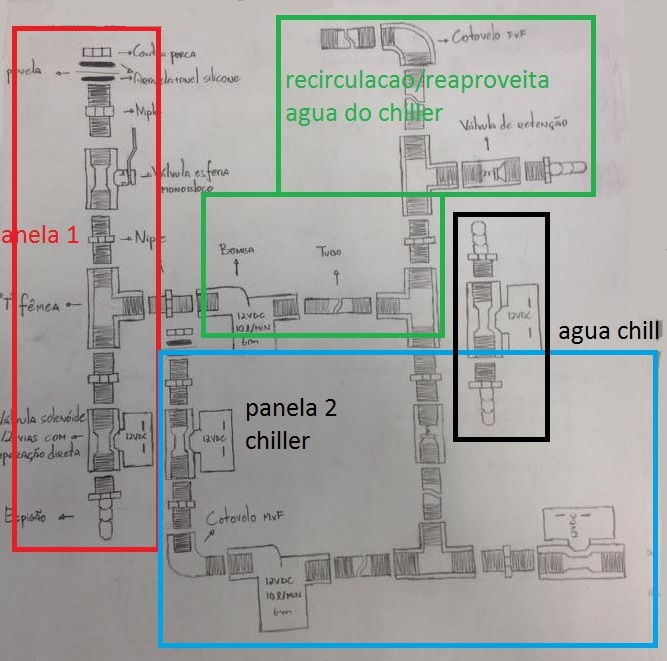
\includegraphics[scale=0.55]{./Resources/conexoes.jpg}
	\captionsetup{justification=centering}
	\caption[Diagrama conceitual das conex�es mec�nicas]{Diagrama conceitual das conex�es mec�nicas}
	\label{conexoes_rascunho}
\end{figure}

\newline

Na figura \ref{mt_cad} � apresentado um diagrama da MT constru�do no software FreeCAD, � qual est�o conectados o resistor de pot�ncia e um niple com veda��o. Tamb�m est�o presentes na figura a v�lvula esfera manual, um \textit{tee} f�mea, uma v�lvula Danfoss EV210B e tr�s niples de conex�o entre estes componentes. O modelo da v�lvula foi obtido a partir do website da Danfoss e importado, enquanto a modelagem dos outros componentes foi desenvolvida na plataforma FreeCAD. Na figura \ref{mt_cad_close} s�o apresentadas em detalhe as conex�es do resistor e do niple � panela e, por isto, a estrutura da mesma foi omitida. Os itens em amarelo s�o contra-porcas, em azul arruelas e, em vermelho an�is de veda��o (\textit{o-rings}).

\begin{figure}[H]
	\centering
	\begin{subfigure}{.46\textwidth}
		\centering
		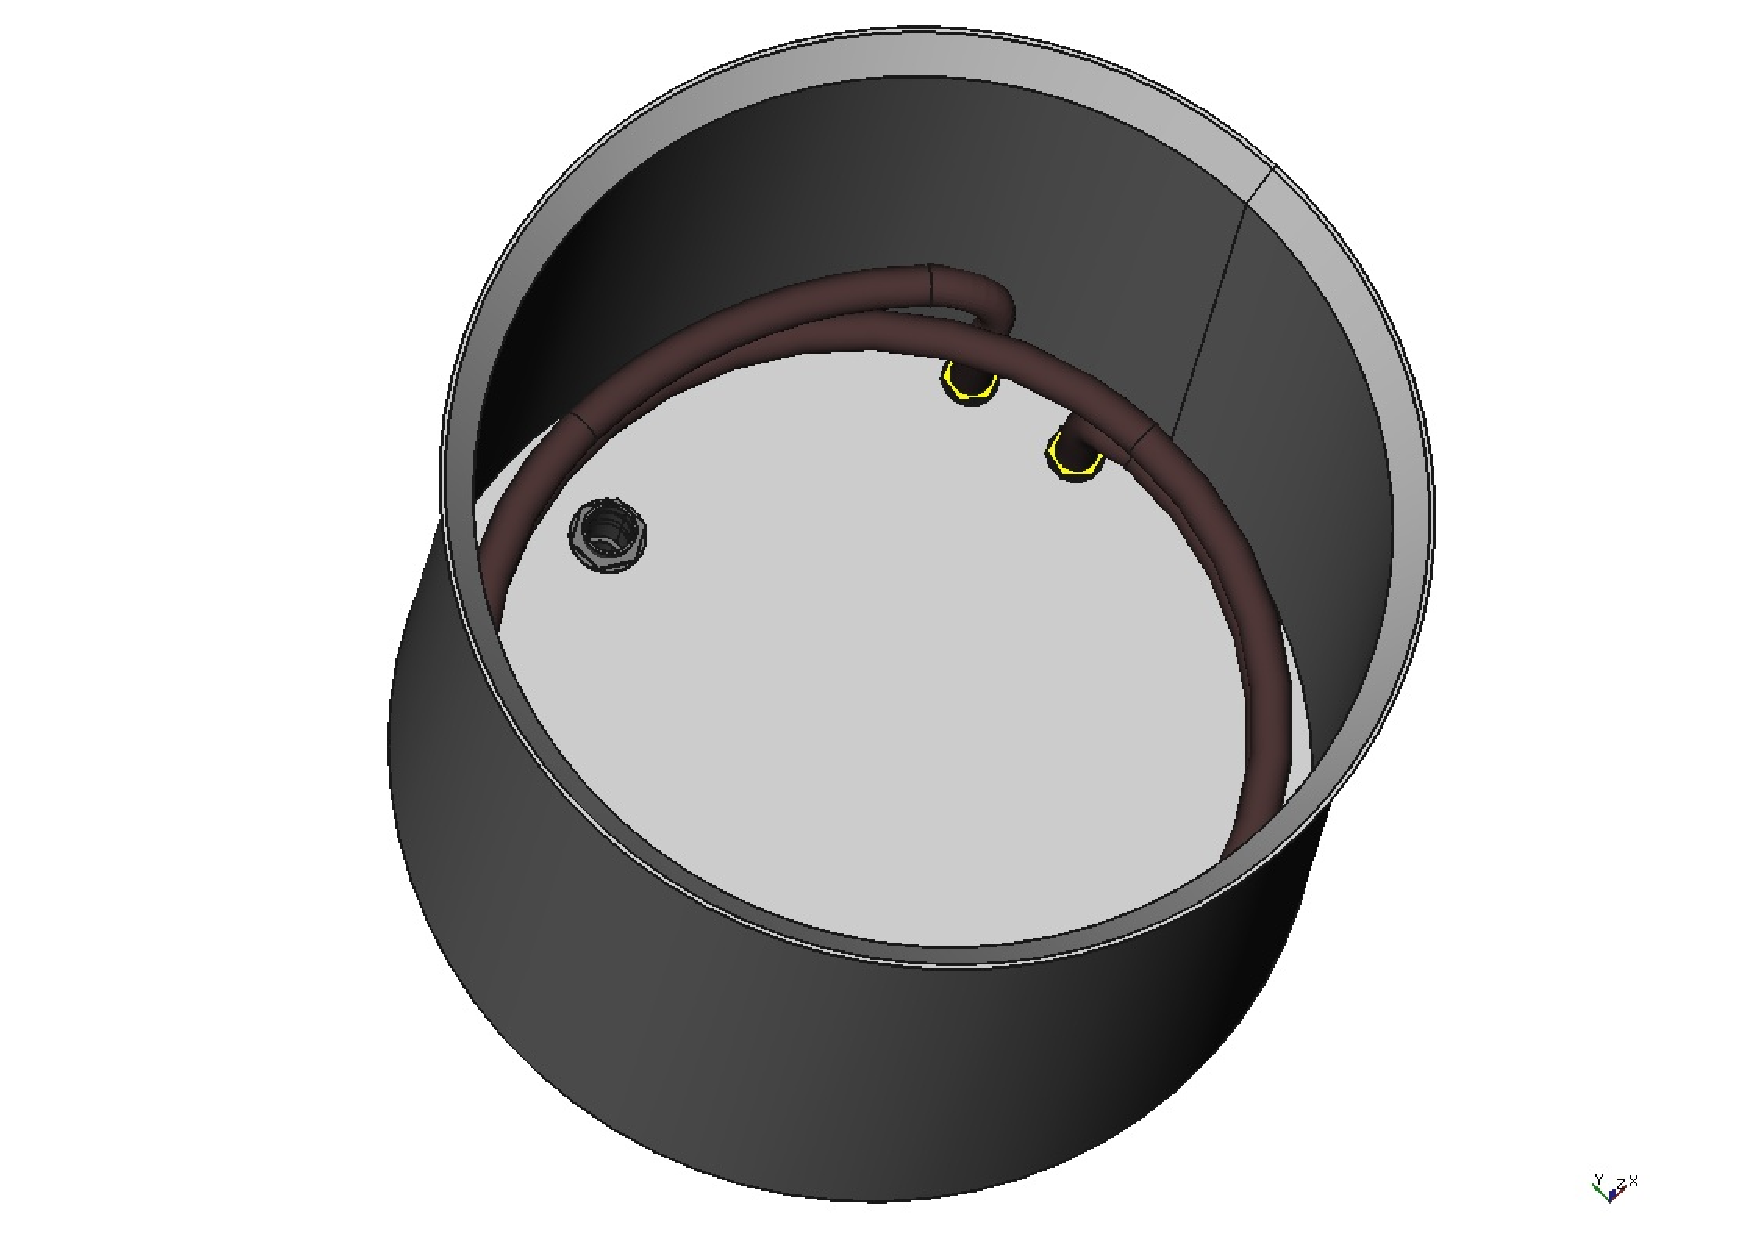
\includegraphics[height=5.5cm]{./Resources/mecsys/mash-tun-top-color.pdf}
		\caption{Vista superior}
		\label{mt_cad:1}
	\end{subfigure}
	\begin{subfigure}{.46\textwidth}
		\centering
		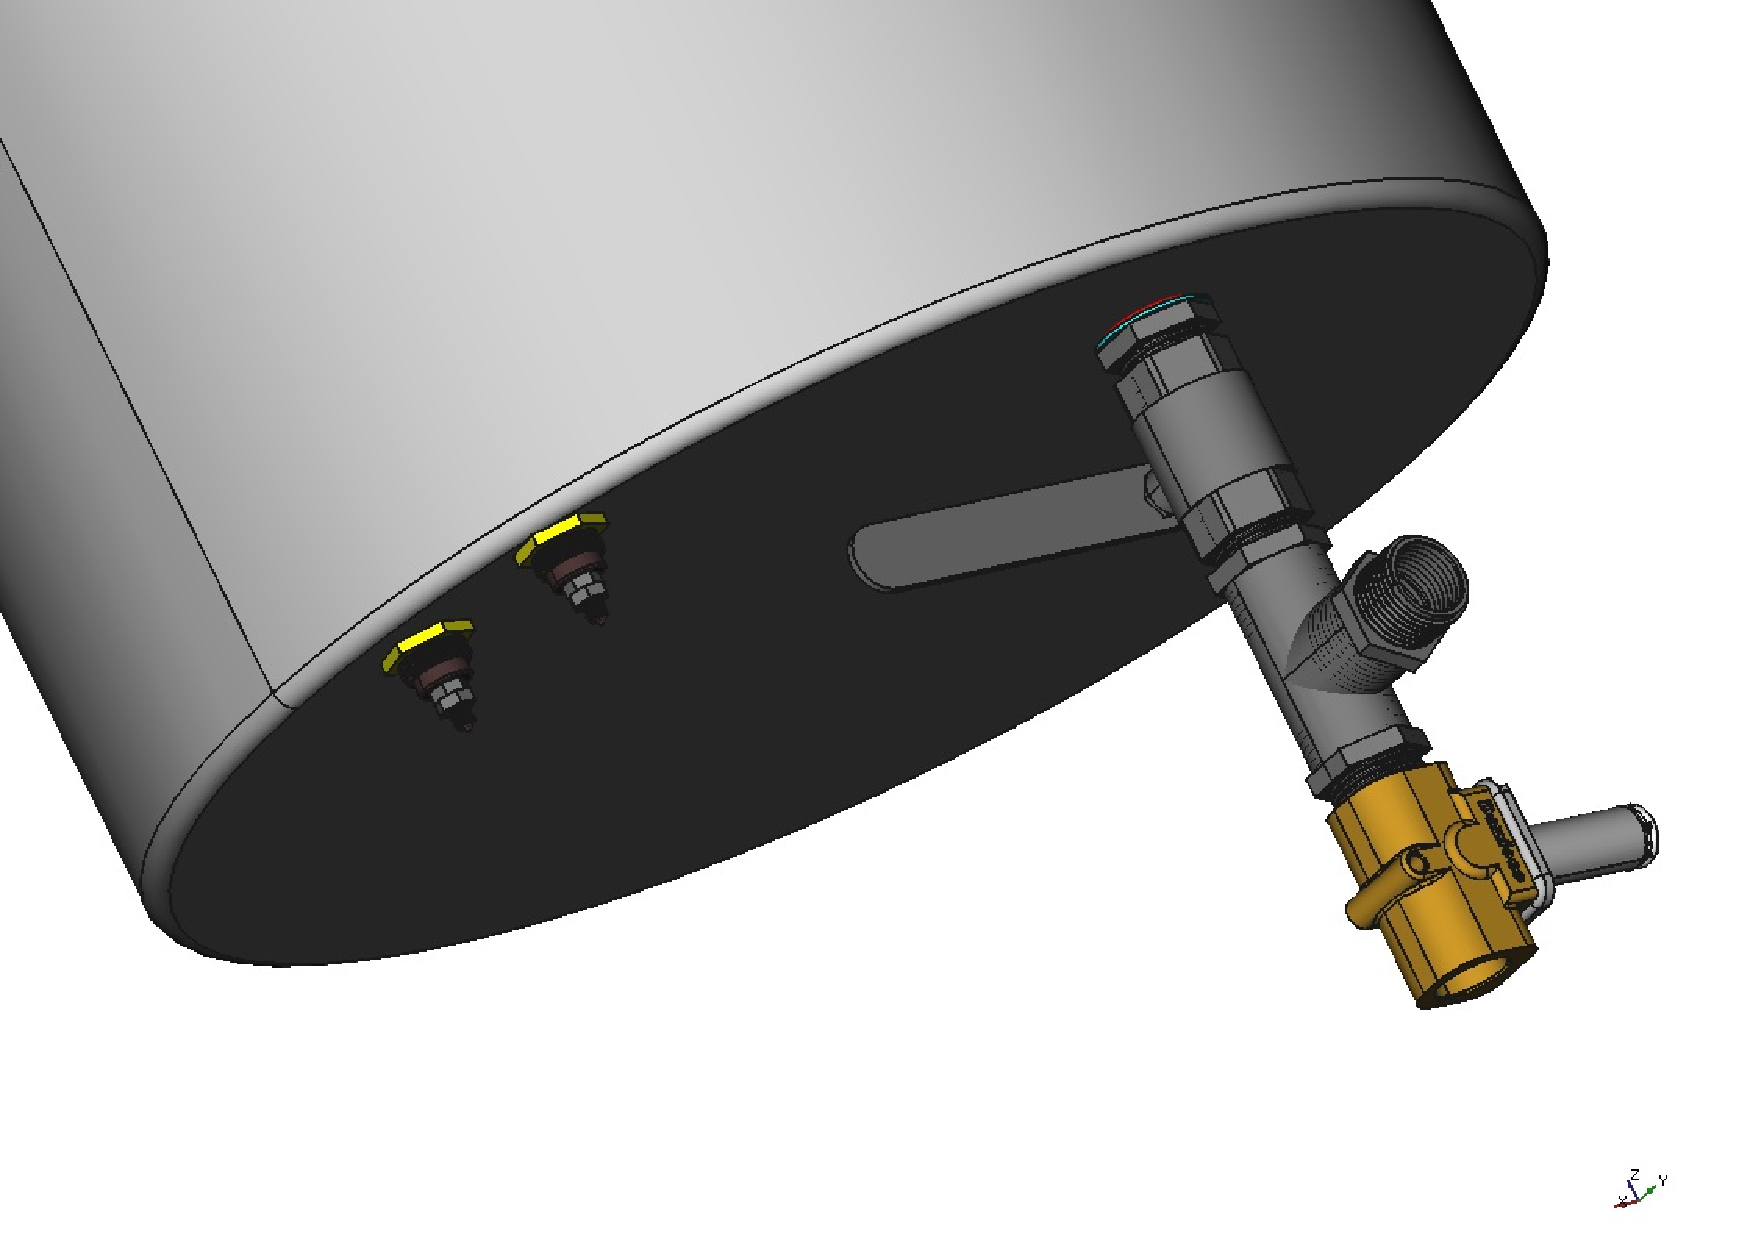
\includegraphics[height=5.5cm]{./Resources/mecsys/mash-tun-bottom-color.pdf}
		\caption{Vista inferior}
		\label{mt_cad:2}
	\end{subfigure}
	\captionsetup{justification=centering}
	\caption[Diagrama da panela de mostura e conex�es]{Diagrama da panela de mostura e conex�es}
	\label{mt_cad}
\end{figure}

\begin{figure}[H]
	\centering
	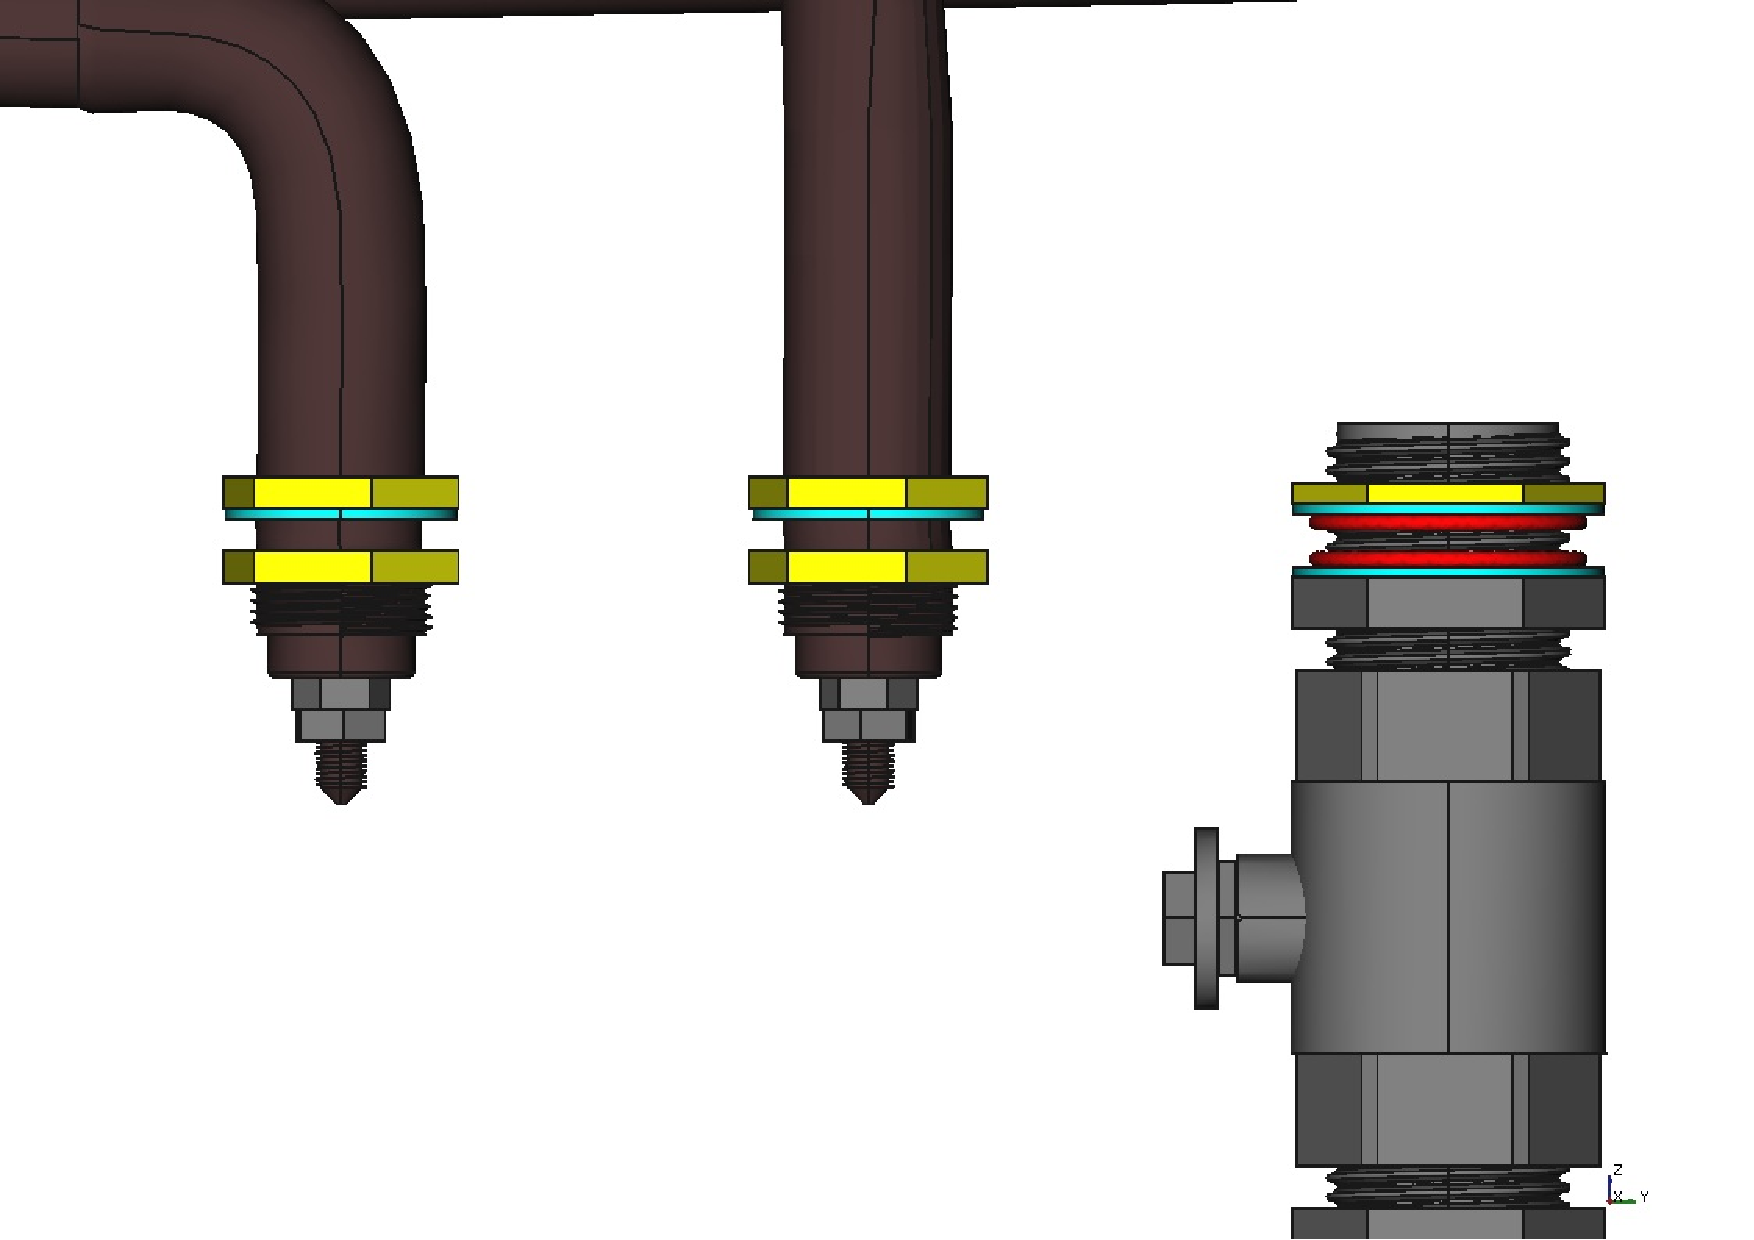
\includegraphics[scale=0.4]{./Resources/mecsys/mash-tun-seal-color.pdf}
	\captionsetup{justification=centering}
	\caption[Detalhes da veda��o da panela de mostura]{Detalhes da veda��o da panela de mostura}
	\label{mt_cad_close}
\end{figure}

\newpage

\subsection{Estrutura met�lica de suporte}

Parte importante do projeto � o dimensionamento da estrutura met�lica de suporte �s panelas, j� que esta � respons�vel n�o somente pelo alojamento do sistema mec�nico como tamb�m pela facilidade de manuten��o. Para defini��o da posi��o das panelas, foram medidas primeiramente as suas alturas e da estrutura de adi��o de l�pulos (que ser� detalhada � parte na se��o \ref{hopbox}) e do \textit{chiller}. Na sequ�ncia, foi estimado um espa�o de manobra entre as duas panelas e uma altura m�nima do ch�o, com base na figura \ref{esboco}. Todas as medidas citadas est�o dispostas na tabela \ref{alturas}.

\begin{center}
	\begin{table}[H]
		\captionsetup{justification=centering}
		\caption[Dimens�es elementos mec�nicos relevantes para o projeto da altura da estrutura met�lica]{Dimens�es elementos mec�nicos relevantes para o projeto da altura da estrutura met�lica}
		\label{alturas}
		\begin{tabular}{ | M{10cm} | M{5cm} |}
			\hline
			\textbf{Descri��o} & \textbf{Altura (cm)} \\ \hline
			Panela BK & 30,0\\ \hline
			Panela MT & 30,0\\ \hline
			\textit{Chiller} & 30,0\\ \hline			
			Estrutura dos l�pulos aberta & 20,0\\ \hline
			V�o livre entre panelas & 20,0\\ \hline
			V�o do \textit{chiller} ao BK & 10,0\\ \hline
			Espa�o entre MT e topo & 10,0\\ \hline
		\end{tabular}
	\end{table}
\end{center}

Somando-se todos os valores da tabela \ref{alturas}, obteve-se que a estrutura met�lica deve ter 1,5m de altura. A largura deve ser de 36,5cm para acomodar as panelas com uma pequena folga e o comprimento escolhido � de 70cm, o que permite alinhar as panelas de maneira n�o conc�ntrica, conforme abordado na se��o \ref{estmec} --- este valor � suficiente, j� que o di�metro somado das duas panelas � de 72cm e � preciso que exista uma intersec��o para permitir o escoamento por gravidade da MT ao BK. Na figura \ref{estmec_cad} � apresentado o projeto da estrutura j� com as prateleiras para acomodar as panelas. Note-se que foram escolhidas cantoneiras de 2" x 1/8" para a constru��o deste equipamento.

\begin{figure}[H]
	\centering
	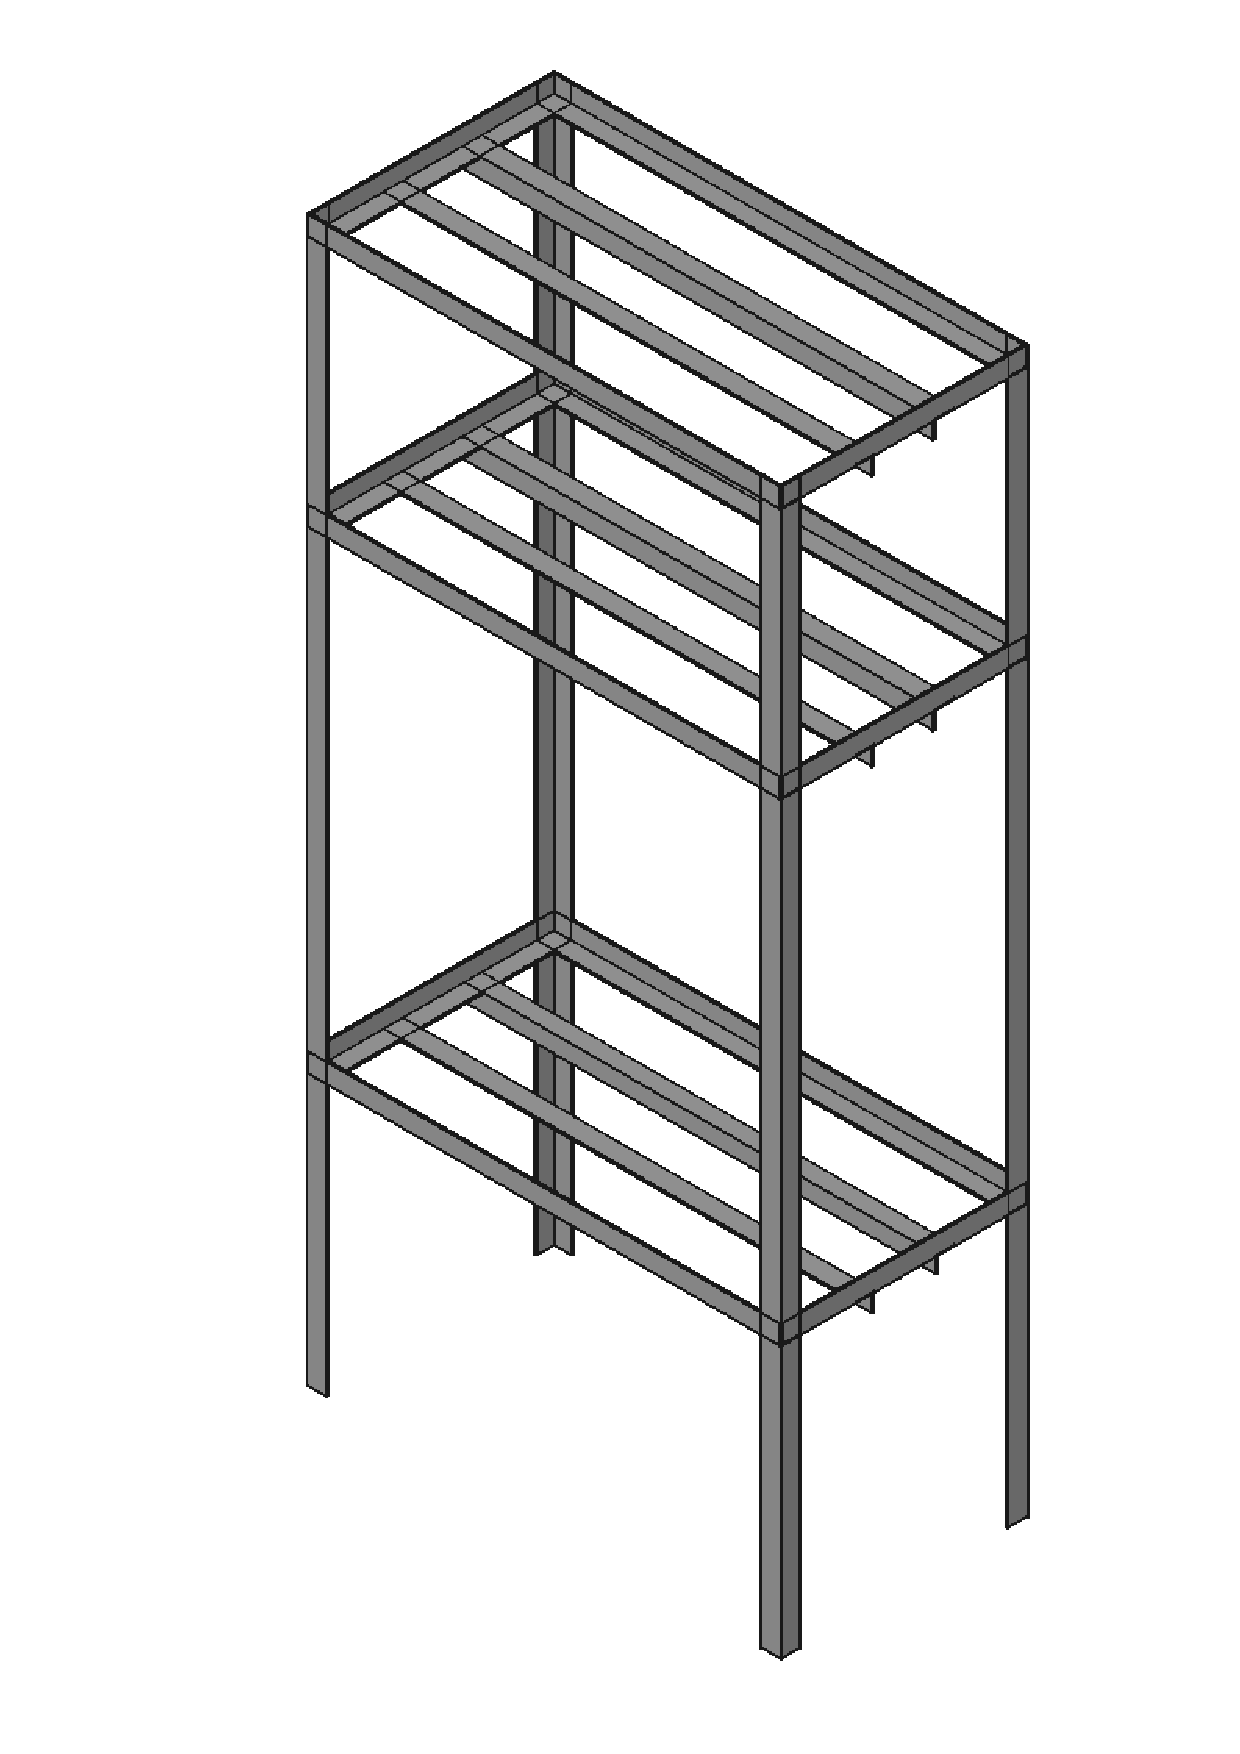
\includegraphics[scale=0.35]{./Resources/mecsys/estmec-freecad.pdf}
	\captionsetup{justification=centering}
	\caption[Projeto da estrutura met�lica]{Projeto da estrutura met�lica}
	\label{estmec_cad}
\end{figure}


%%%%%%%%%%%%%%%%%%%%%%%%%%%%%%%%%%%%%%%%%%%%%%%%%%%%%%%%%%%%%%%%%%%%%%%%%%

\section{Estrutura de adi��o de l�pulos}
\label{hopbox}
%Devido � necessidade de adicionar l�pulos � receita em propor��es e tempos predefinidos, foi necess�rio o projeto de uma estrutura autom�tica de adi��o de l�pulos. Em fun��o das in�meras possibilidades de combina��es de l�pulos e temporiza��es, a escolha natural do projeto foi uma estrutura que permita esta flexibilidade --- uma caixa com oito compartimentos separados para adi��o sequencial destes insumos. Com base em um pacote de l�pulos em \textit{pellets} de 50g, estimou-se que seu volume � de $160cm^3$ e, sabendo-se que uma receita de 20l dificilmente utiliza uma quantidade maior do que 400g de l�pulos, a decis�o tomada foi a de que cada um dos 8 compartimentos deveria ter os $160cm^3$ necess�rios para acomodar 50g. Para confirmar que 400g � uma quantidade razo�vel, foi seguido o c�lculo de IBU de \cite{palmer}, detalhado no ap�ndice \ref{Ap�ndice C}.

Fixando a altura do compartimento em 10,0cm foram escolhidos valores de comprimento e largura de 16,0cm e 8,0cm respectivamente, assumindo inicialmente que as paredes das divis�rias tem espessura desprez�vel. A equa��o para volume de um prisma e a escolha das dimens�es s�o demonstradas em \ref{eq_hop_vini}:

\begin{subequations}
	\label{eq_hop_vini}
	\begin{align}
		V &= l\cdot w\cdot h = V_{50g}\cdot 8 \\
		&= l\cdot w\cdot 10 = 160\cdot 8 \nonumber \\
		l\cdot w\cdot &= 128, fixando \quad l = 16cm \quad \therefore \nonumber \\
		w &= 128/16 = 8cm \quad e \\
		w_{compartimento} &= l/8 = 16/8 = 2cm
	\end{align}
\end{subequations}

Posteriormente aos c�lculos de \ref{eq_hop_vini}, durante o projeto no software FreeCAD, observou-se que a assump��o de espessura desprez�vel � falsa e um retrabalho nas medidas do compartimento levou �s dimens�es externas finais de 18,0cm x 8,4cm x 10,0cm; as paredes externas tendo espessura de 3,0mm e as internas de 2,0mm. A figura \ref{caixa_cinza} esbo�a as dimens�es externas da caixa e a figura \ref{corpo_hopbox} apresenta o corpo da estrutura.

\begin{figure}[H]
	\centering
	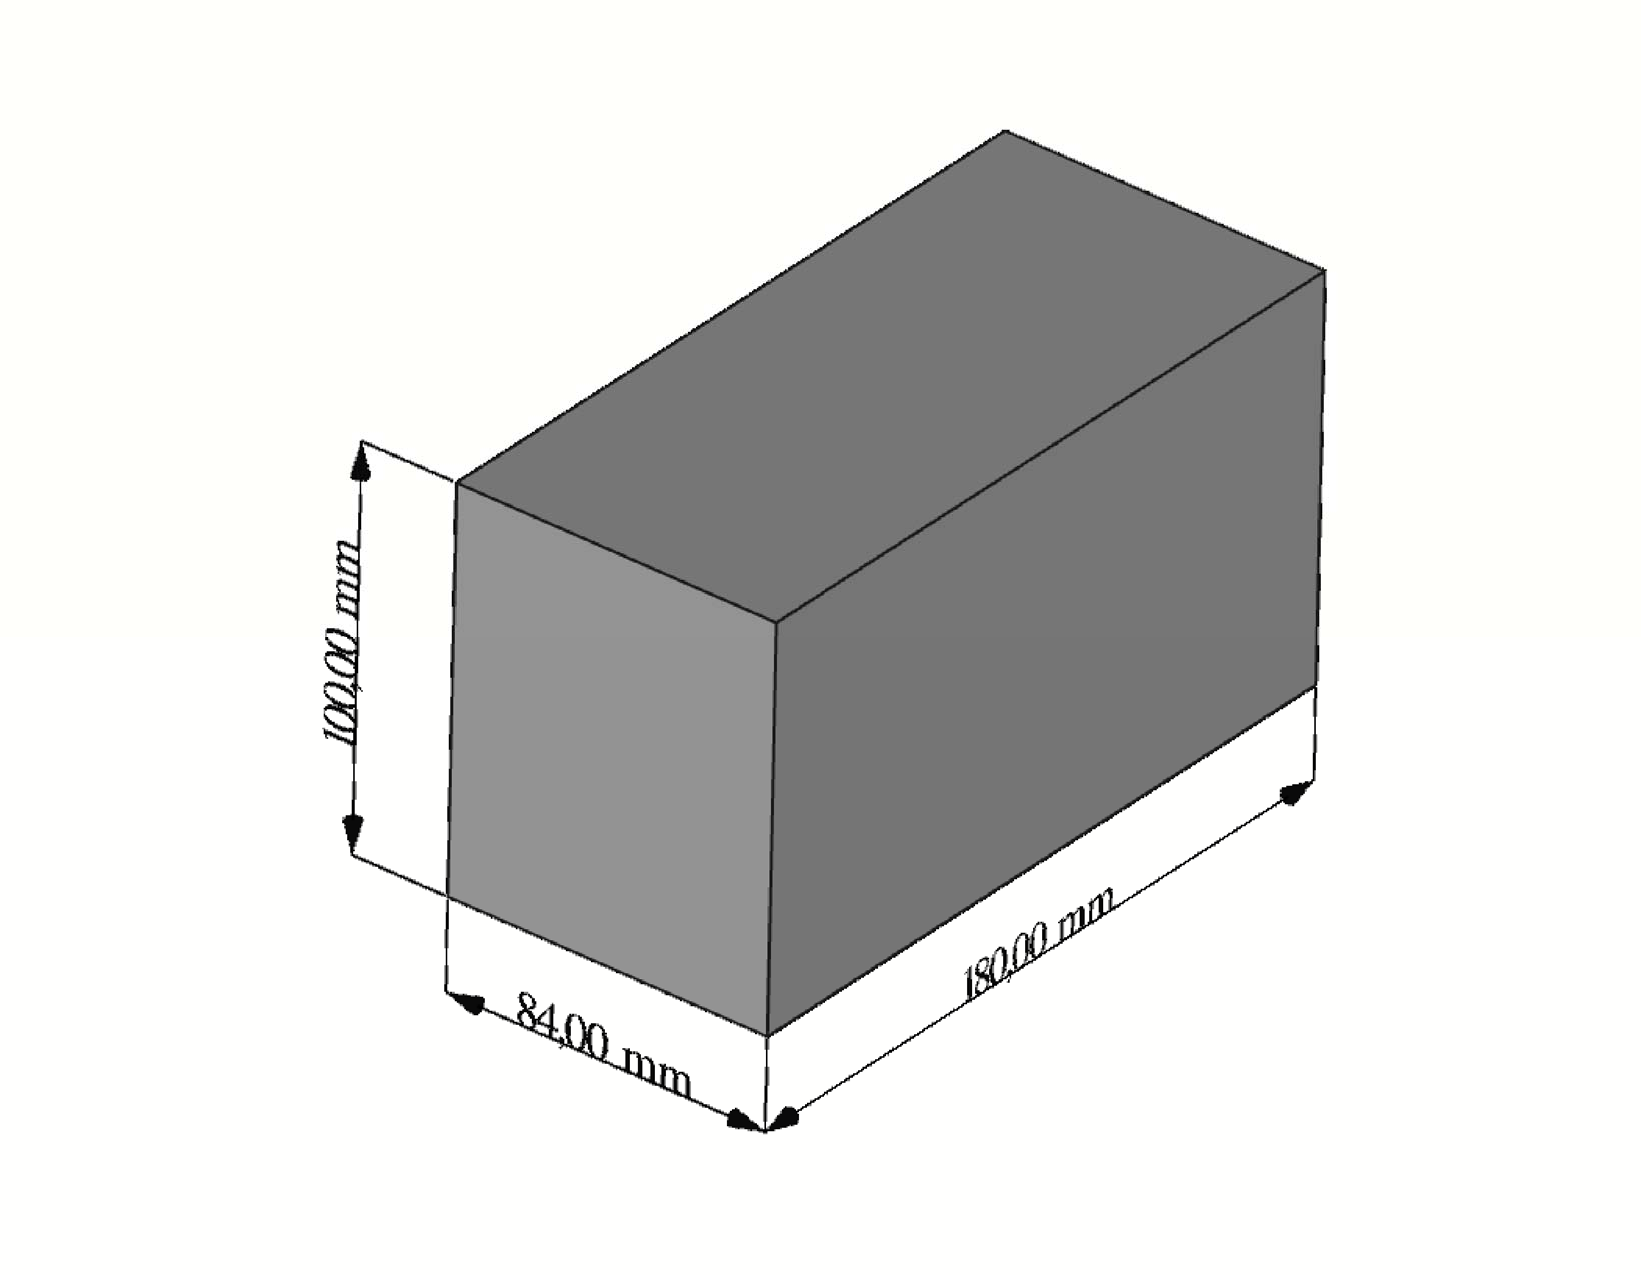
\includegraphics[scale=0.35]{./Resources/estLup/caixa_lupulos(1).pdf}
	\captionsetup{justification=centering}
	\caption[Dimens�es da estrutura de adi��o de l�pulos]{Dimens�es da estrutura de adi��o de l�pulos}
	\label{caixa_cinza}
\end{figure}

\begin{figure}[H]
	\centering
	\begin{subfigure}{.46\textwidth}
		\centering
		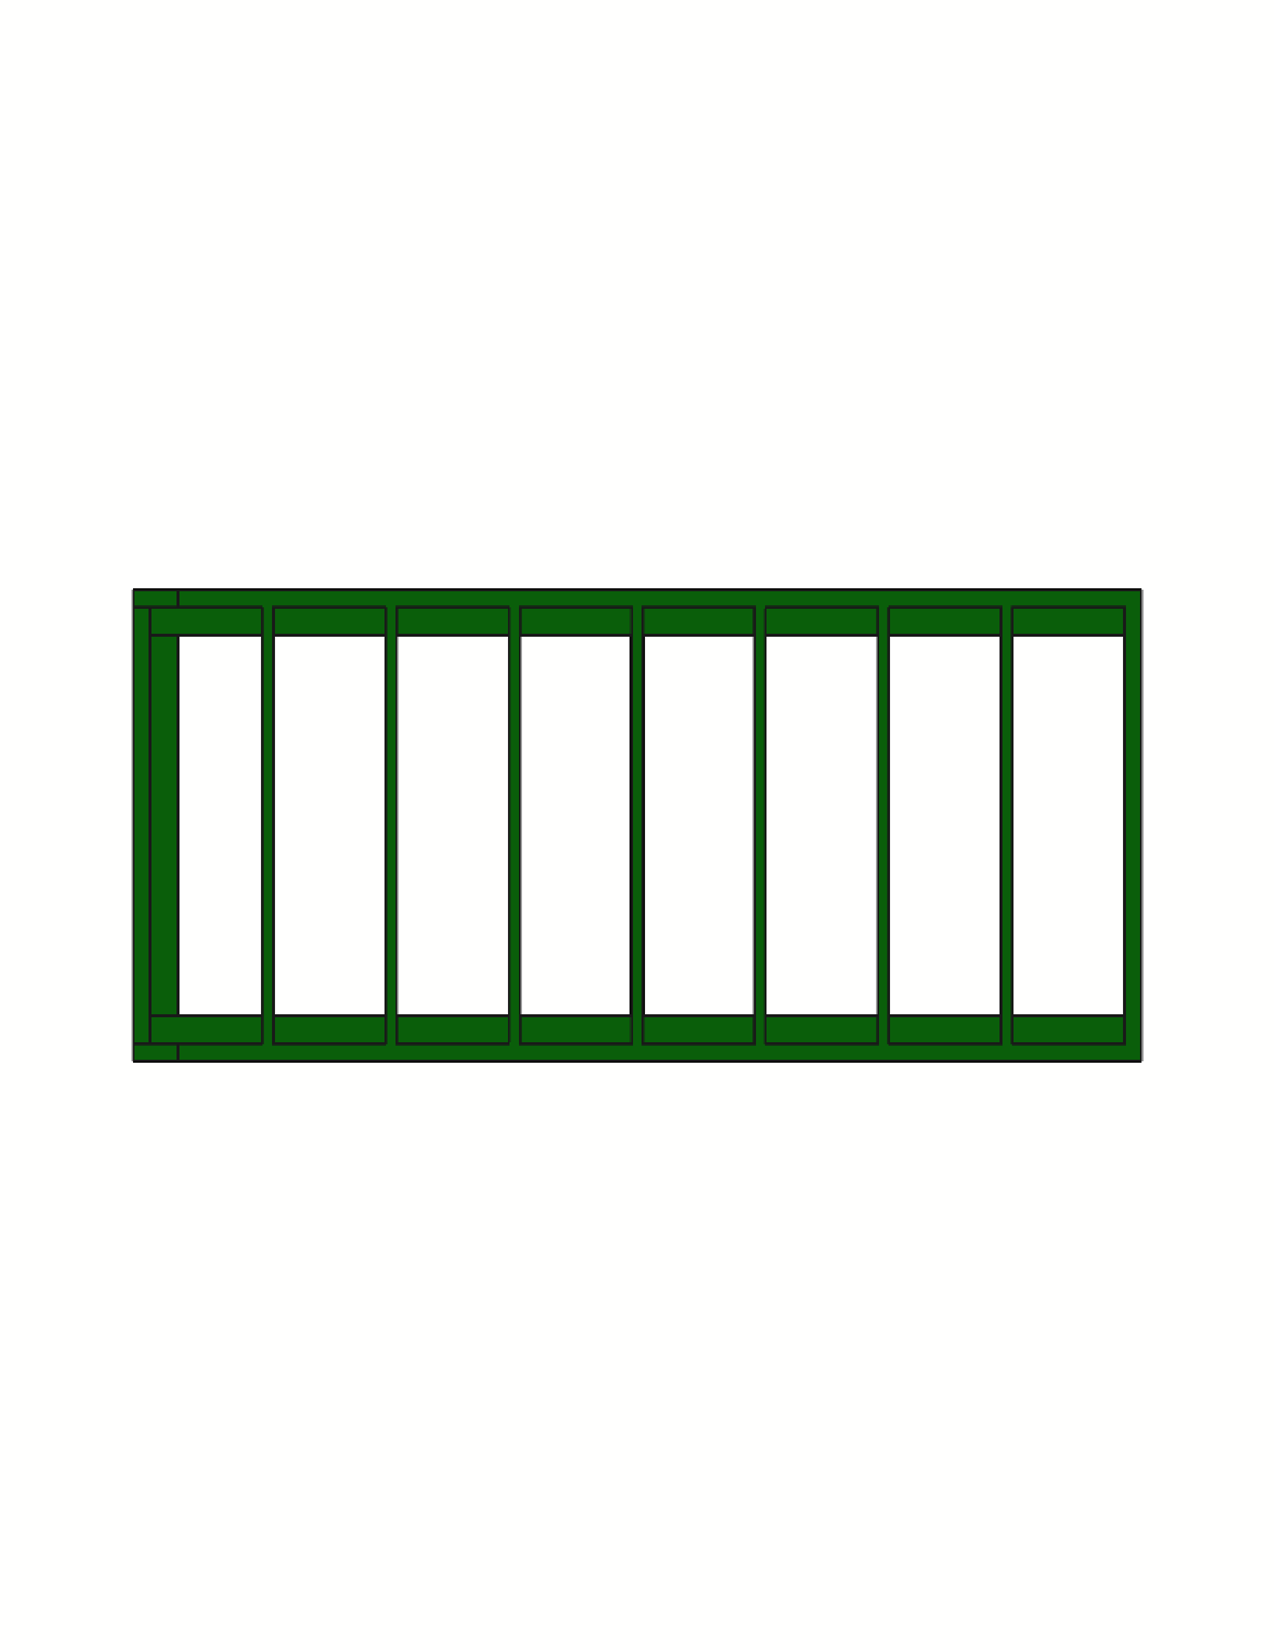
\includegraphics[height=7.5cm]{./Resources/estLup/caixa_lupulos(2).pdf}
		\caption{Vista superior}
		\label{corpo_hopbox:1}
	\end{subfigure}
	\begin{subfigure}{.46\textwidth}
		\centering
		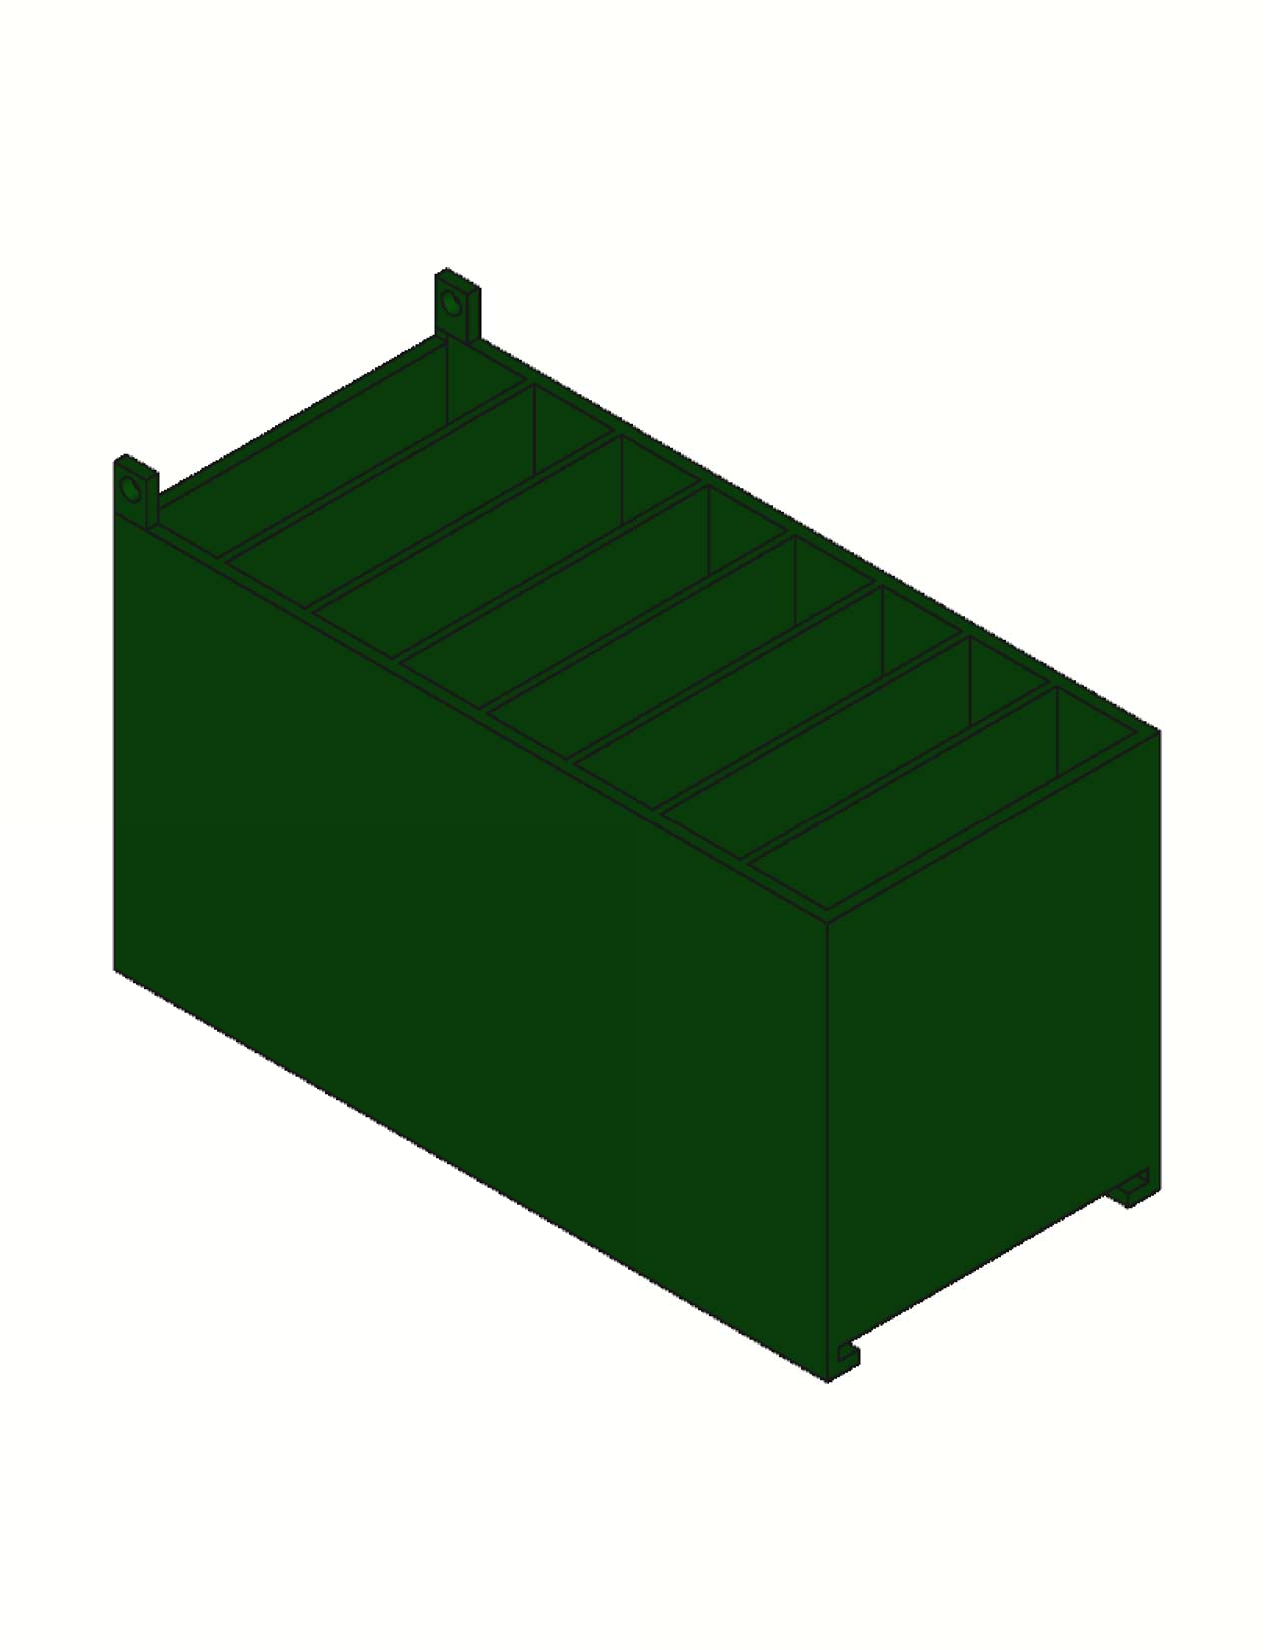
\includegraphics[height=7.5cm]{./Resources/estLup/caixa_lupulos(3).pdf}
		\caption{Vista axiom�trica}
		\label{corpo_hopbox:2}
	\end{subfigure}
	\captionsetup{justification=centering}
	\caption[Corpo da estrutura de adi��o de l�pulos]{Corpo da estrutura de adi��o de l�pulos}
	\label{corpo_hopbox}
\end{figure}

Foram projetadas duas portinholas: uma na face superior da caixa, para reabastecimento manual dos l�pulos, com uma al�a e fixada na caixa por dois pinos, de modo que a abertura desta tampa � um movimento de rota��o e; uma na face inferior, para adi��o autom�tica, de correr, de modo que a abertura � um movimento de transla��o; ambas est�o ilustradas na figura \ref{tampas_hopbox}.

\begin{figure}[H]
	\centering
	\begin{subfigure}{.46\textwidth}
		\centering
		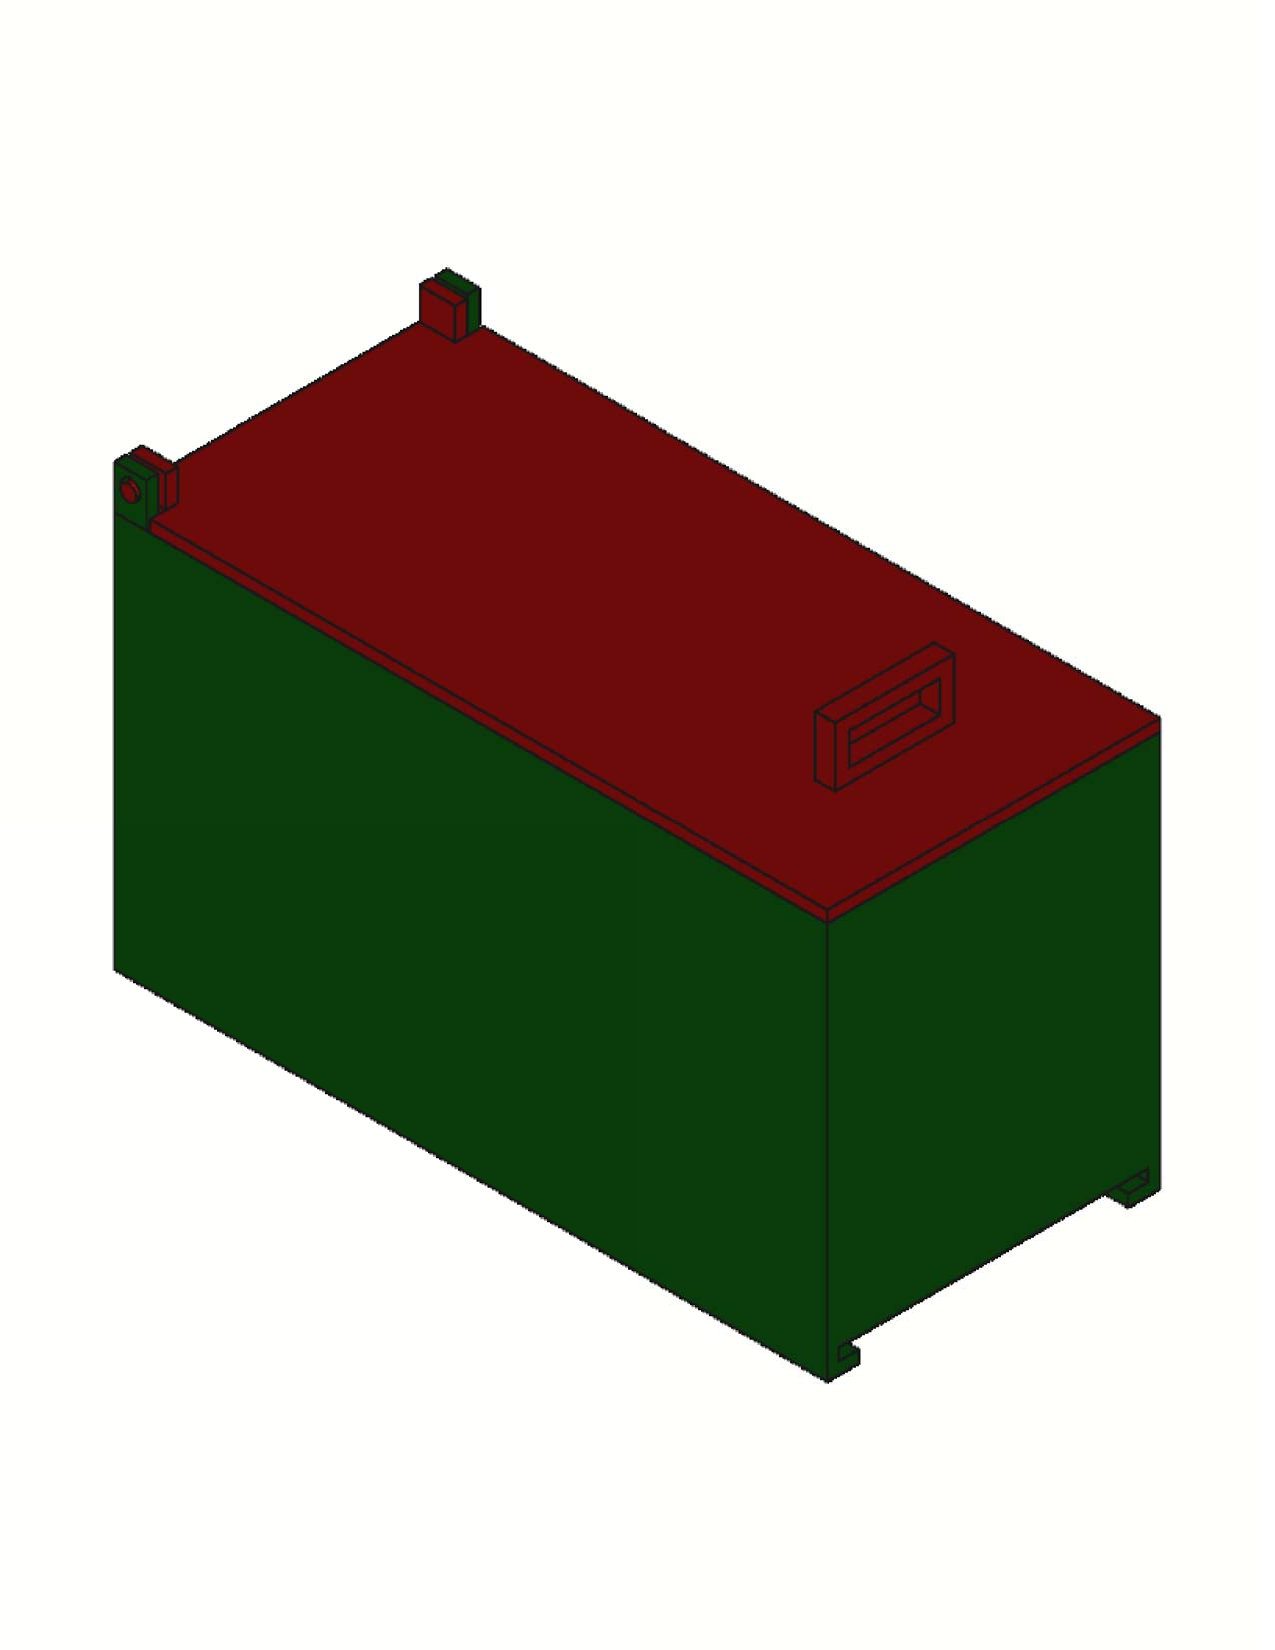
\includegraphics[height=7.5cm]{./Resources/estLup/caixa_lupulos(4).pdf}
		\caption{Tampa manual para reabastecimento}
		\label{tampas_hopbox:1}
	\end{subfigure}
	\begin{subfigure}{.46\textwidth}
		\centering
		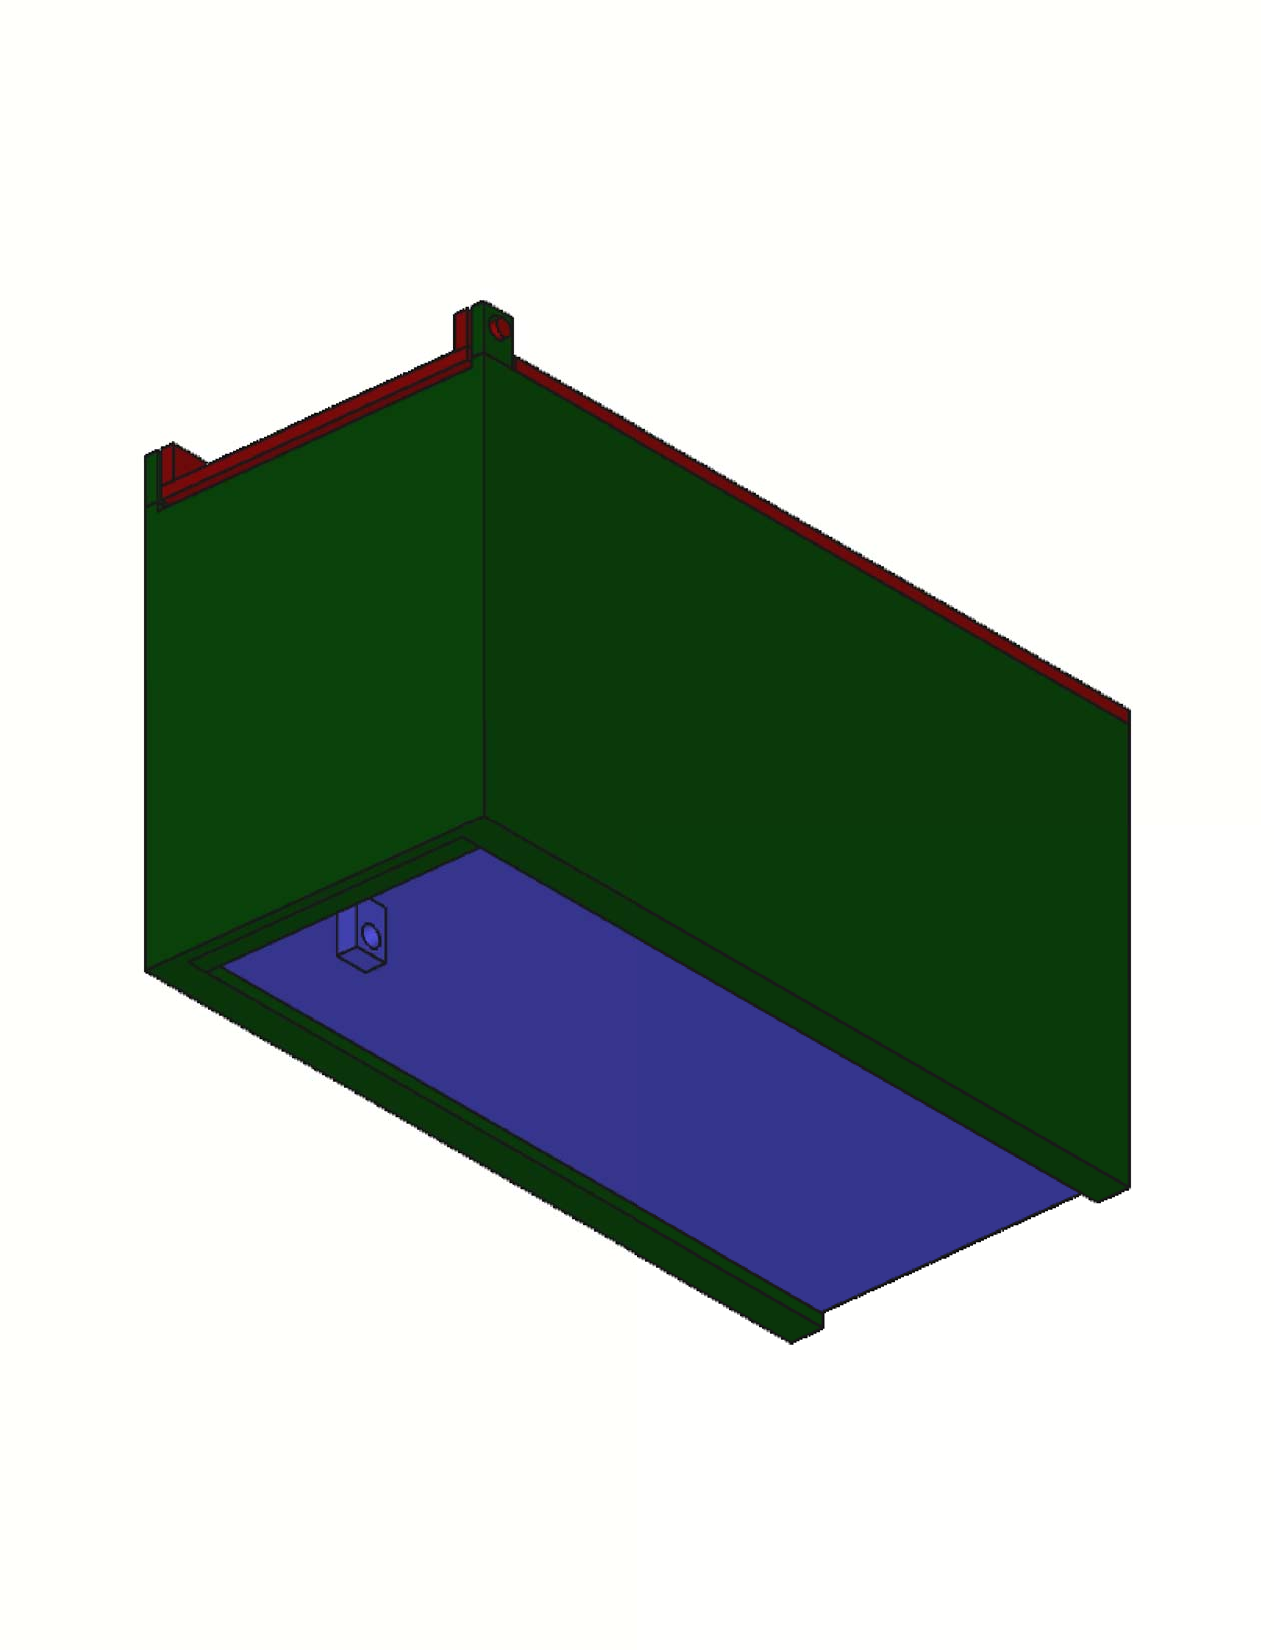
\includegraphics[height=7.5cm]{./Resources/estLup/caixa_lupulos(5).pdf}
		\caption{Tampa para adi��o autom�tica dos l�pulos}
		\label{tampas_hopbox:2}
	\end{subfigure}
	\captionsetup{justification=centering}
	\caption[Tampas da estrutura de adi��o de l�pulos]{Tampas da estrutura de adi��o de l�pulos}
	\label{tampas_hopbox}
\end{figure}

Duas varetas de comprimento $l_1$ e $l_2$ s�o ligadas ao encaixa da tampa de correr, representada em azul na figura \ref{tampas_hopbox:2}, e a elas � acoplado um servo-motor cujo �ngulo de opera��o $\theta$ define a abertura --- ou deslocamento --- da tampa, definido por $d$. A figura \ref{varetas} esquematiza as liga��es.

\begin{figure}[H]
	\centering
	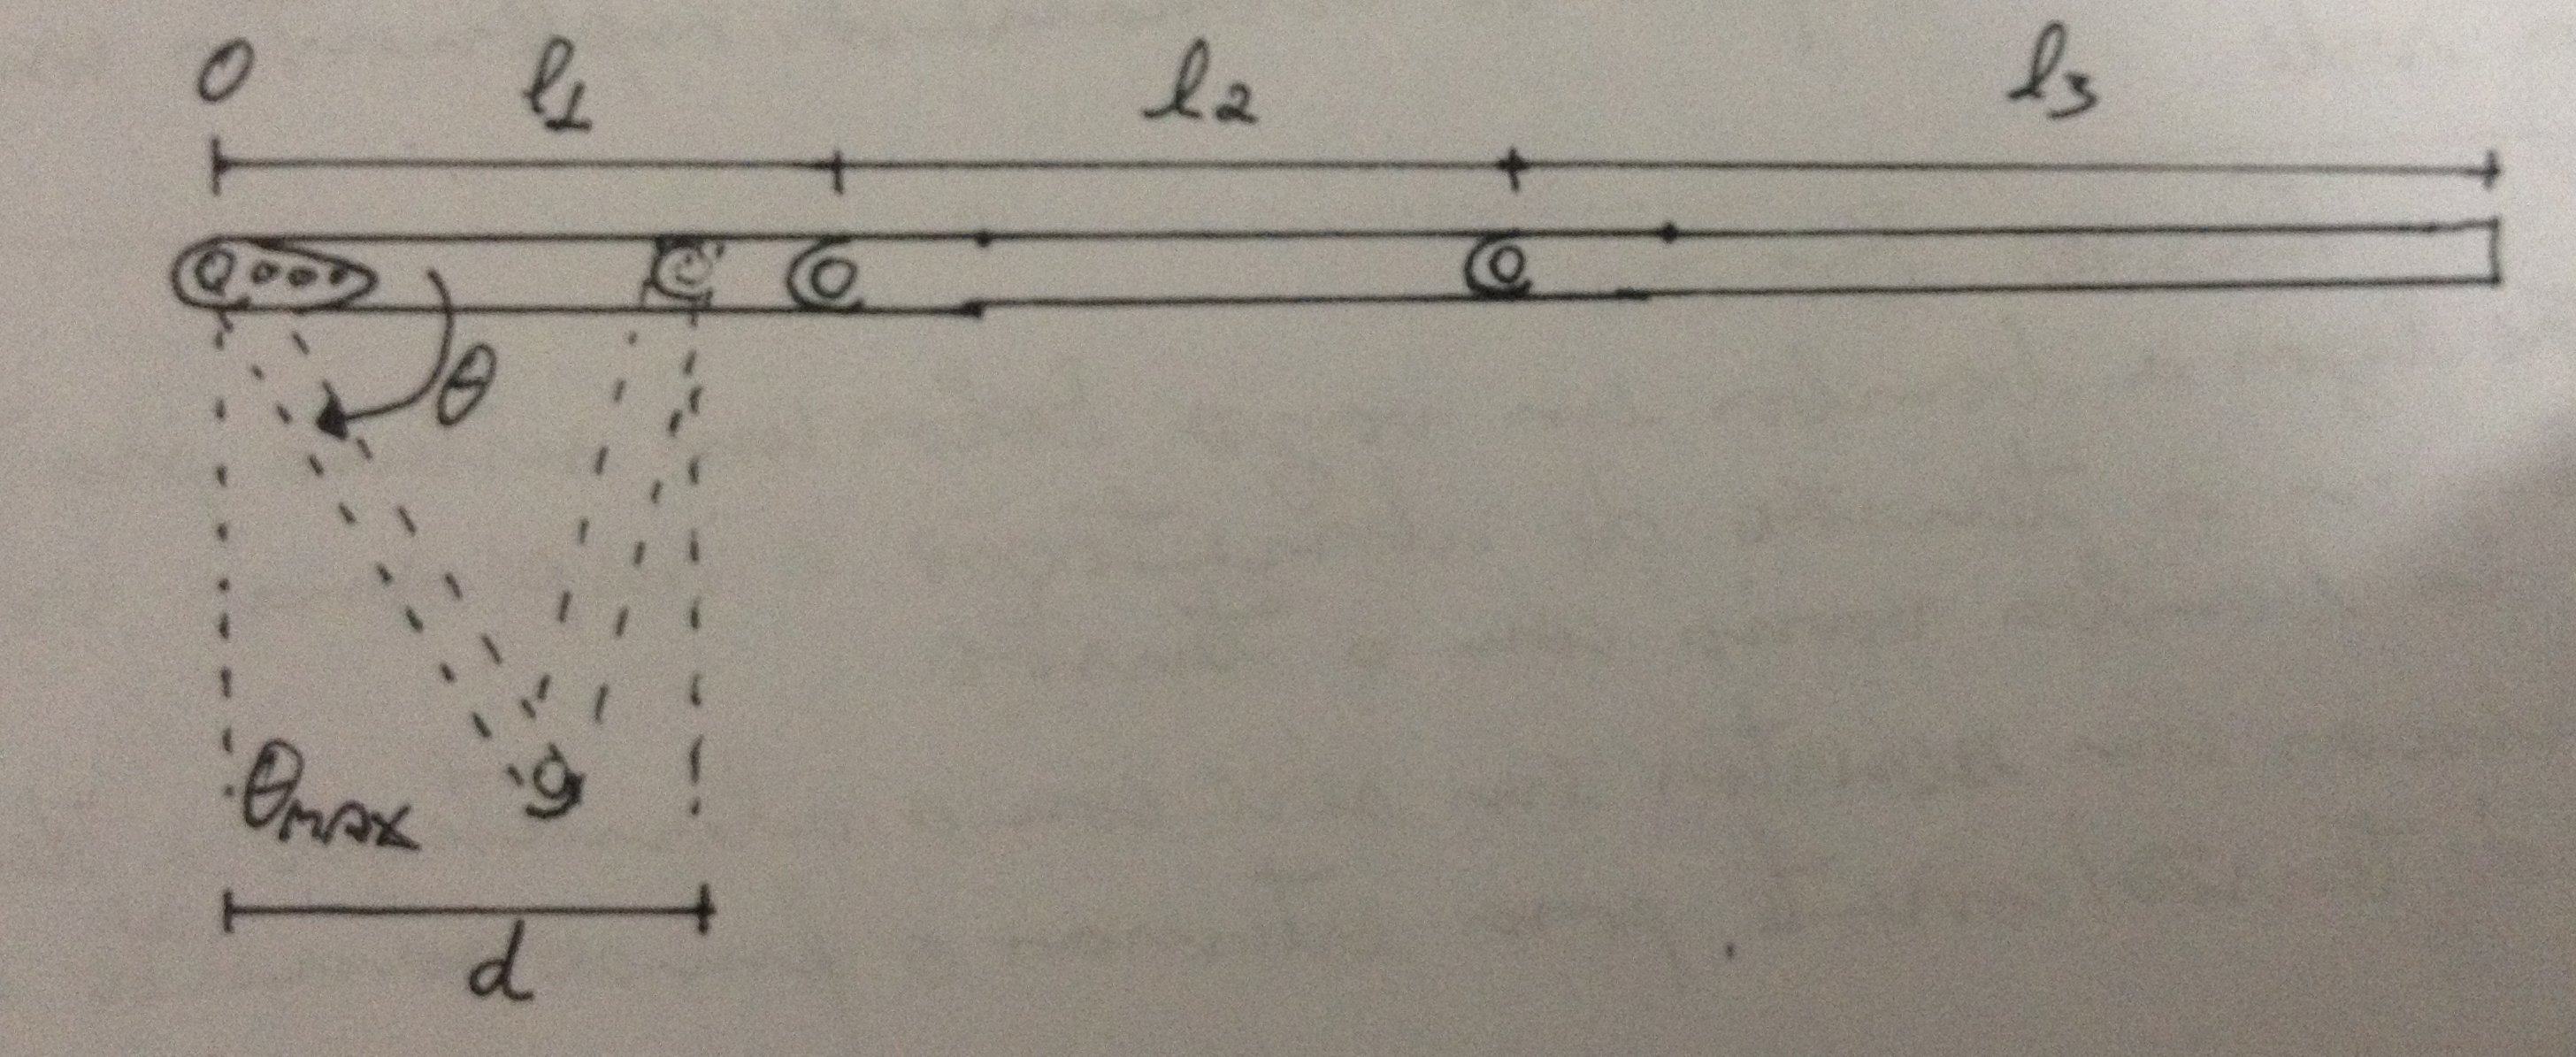
\includegraphics[scale=0.1]{./Resources/estLup/esquema-varetas.jpg}
	\captionsetup{justification=centering}
	\caption[Esquema de liga��o das varetas � tampa de correr]{Esquema de liga��o das varetas � tampa de correr}
	\label{varetas}
\end{figure}

Sendo o comprimento da tampa igual a $l_3$, a condi��o em \ref{eq_varetas} deve ser satisfeita para que a excurs�o m�xima de abertura da caixa possa ser atingida. � poss�vel demonstrar com o aux�lio da Lei dos Cossenos, em \ref{eq_cossenos} que $l_1 = l_2 = l$ para que a m�nima abertura da caixa possa ser atingida.

\begin{align}
	\label{eq_varetas}
	l_1 + l_2 \geq l_3
\end{align}

\begin{align}
	\label{eq_cossenos}
	&l_2^2 = d^2 + l_1^2 - 2dl_1\cdot cos(\theta) \\
	&se \quad \theta = 90\si{\degree} \rightarrow d = 0 \therefore \nonumber\\
	\label{res_cossenos}
	&l_2^2 = l_1^2 \rightarrow l_2 = l_1 = l
\end{align}

A taxa m�xima de deslocamento em fun��o do �ngulo do servo motor � expressa em \ref{eq_desl}:

\begin{align}
	\label{eq_desl}
	\frac{dl_3}{d\theta} = \frac{2l}{90\si{\degree}}
\end{align}

Entretanto, quanto maior o valor desta taxa, menor � a resolu��o de abertura da caixa, portanto obtem-se que o menor valor poss�vel de $l$, a partir de \ref{eq_varetas} � $l = l_3/2$. Assim sendo, a taxa de deslocamento calculada a partir de \ref{eq_desl} � de $2mm/\si{\degree}$.

Embora o valor te�rico de $\theta$ seja $90\si{\degree}$, na pr�tica, devido ao encaixe entre tampa e vareta n�o ser na extremidade, este valor � reduzido. Tal fato n�o deve ser negligenciado, uma vez que isto pode for�ar a opera��o do servo-motor. Sabe-se pelo projeto executado no FreeCAD que a dist�ncia da borda ao encaixe da tampa � de 2,3cm portanto, com o aux�lio da Lei dos Cossenos, obt�m-se que $\theta_{max} = 82\si{\degree}$. Quanto ao valor m�nimo n�o h� preocupa��o , j� que a abertura da caixa ter� uma excurs�o reduzida em 2,3cm com rela��o ao seu comprimento. As varetas n�o foram calculadas novamente pois julgou-se uma boa pr�tica essa redu��o, que evita que a tampa caia da caixa quando em m�xima excurs�o. A figura \ref{completa_hopbox} apresenta o esquema completo de constru��o da estrutura de adi��o de l�pulos.

\begin{figure}[H]
	\centering
	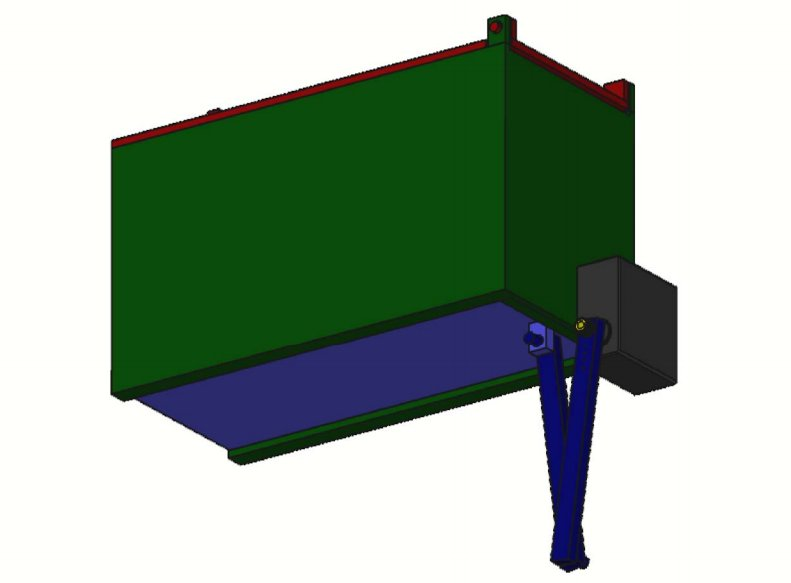
\includegraphics[scale=0.25]{./Resources/estLup/final.jpg}
	\captionsetup{justification=centering}
	\caption[Estrutura de adi��o de l�pulos]{Estrutura de adi��o de l�pulos}
	\label{completa_hopbox}
\end{figure}



%%%%%%%%%%%%%%%%%%%%%%%%%%%%%%%%%%%%%%%%%%%%%%%%%%%%%%%%%%%%%%%%%%%%%%%%%%

\section{Sistema de controle de vers�o}
%Para facilitar o desenvolvimento e a documenta��o de \textit{softwares}, duas ferramentas foram adotadas al�m do acesso ao sistema embarcado via SSH: \textit{Cloud9}, cujo uso � descrito na se��o \ref{c9} e \textit{Git/GitHub}, na se��o \ref{ghb}.

\section{\textit{Cloud9}}
\label{c9}

\textit{Cloud9} � um IDE do tipo \textit{software as a service} ou software como um servi�o (SaaS), ou seja, um software que est� na nuvem e cujo acesso � feito por meio de um navegador de internet. Embora o servi�o padr�o seja hospedado nos pr�prios servidores da \textit{Cloud9 IDE Inc.}, um SDK � disponibilizado, no qual est� incluso o n�cleo do projeto como c�digo-aberto, livre para uso n�o comercial e desenvolvido em Node.js. Isto possibilitou a hospedagem do servi�o do \textit{Cloud9} localmente na BBB\cite{c9_license}. Esta � uma n�tida vantagem para uma plataforma \textit{headless} --- sem perif�ricos do tipo \textit{human interface device} (HID) --- e com acesso � rede, a exemplo da BBB neste projeto, pois permite a programa��o direta no dispositivo por meio de uma interface gr�fica via web.

Tanto o n�cleo quanto as informa��es para instala��o podem ser encontradas no reposit�rio do projeto do \textit{GitHub} (\url{https://github.com/c9/core}). A primeira tentativa de instala��o realizado na BBB � apresentado na caixa de c�digo-fonte \ref{c9install}:

\lstset{language=bash}
\begin{lstlisting}[frame=single, basicstyle=\linespread{0.85}\ttfamily, caption=Primeira tentativa de instala��o do \textit{Cloud9 IDE core} na BBB, label=c9install]
cd ~/
git clone git://github.com/c9/core.git c9sdk
cd c9sdk
scripts/install-sdk.sh
\end{lstlisting}

Ao tentar executar a aplica��o apontando para o diret�rio \textit{/var/www} como diret�rio de projeto, ou seja, o diret�rio raiz ao qual o \textit{Cloud9} tem acesso, n�o foi poss�vel acessar os arquivos uma vez que o diret�rio em si pertencia ao usu�rio \textit{www-data} e os arquivos ao \textit{root}.

Ao rodar a aplica��o como administrador, outros erros ocorreram, o que levou � tentativa de instalar outro script presente no endere�o \url{https://github.com/c9/install} do reposit�rio do \textit{Cloud9}, que permite a conex�o da IDE a um servidor SSH. Ainda assim, os erros persistiram, o que levou � abertura de uma quest�o em \url{https://github.com/c9/core/issues/143}, na qual est� descrito o processo adotado para solucionar o problema. Na caixa de c�digo-fonte \ref{c9install_really} � apresentado o processo de instala��o executado com sucesso:

\lstset{language=bash}
\begin{lstlisting}[frame=single, basicstyle=\linespread{0.85}\ttfamily, caption=Instala��o bem sucedida do \textit{Cloud9 IDE core} na BBB, label=c9install_really]
cd ~/
wget --no-check-certificate https://raw.githubusercontent.com/c9/install/master/install.sh
sudo bash install.sh
\end{lstlisting}

Note-se que muitas tentativas foram executadas para obter o resultado final esperado, por isso em caso de tentativa de reprodu��o do processo de instala��o aqui descrito � recomendado tentar usar somente o processo da caixa de c�digo \ref{c9install_really} e, em caso de falha, partir para a etapa descrita anteriormente. Ainda assim, outro processo de instala��o mais direto e que deve ser tentado prioritariamente ao aqui descrito, mas que n�o foi testado, est� descrito em \url{https://cloud9-sdk.readme.io/docs/running-the-sdk}.

Para rodar a aplica��o no background e continuar executando mesmo ap�s desconectar da sess�o SSH, � preciso executar o servidor do \textit{Cloud9} como root usando o comando descrito na caixa \ref{c9start}. O par�metro \textit{-l} indica o endere�o de IP do servidor, \textit{-p} a porta, \textit{-a} usu�rio e senha e \textit{-w} o diret�rio de trabalho. Tamb�m s�o feitas redire��es das sa�das \textit{stdout} e \textit{stderr} para os arquivos \textit{/var/www/log/cl9.out} e \textit{/var/www/log/cl9.err}, respectivamente.

\lstset{language=bash}
\begin{lstlisting}[frame=single, basicstyle=\linespread{0.85}\ttfamily, caption=Execu��o do \textit{Cloud9}, label=c9start]
sudo su #precisa ser root
cd /home/debian #pasta na qual esta instalado o Cloud9
nohup node c9sdk/server.js -l 143.107.xxx.xxx -p xxxx -a usuario:senha -w /var/www/ > /var/www/log/cl9.out 2> /var/www/log/cl9.err < /dev/null &
\end{lstlisting}

Ao realizar o acesso pelo navegador usando o IP e porta selecionados, ou seja, digitando \textit{IP:porta} na URL do navegador, o resultado � apresentado na figura \ref{c9ide}. Note-se que o ambiente apresentado � a configura��o de IDE completa, mas que � completamente personaliz�vel, al�m de existirem outros \textit{presets}, dentre os quais um modo minimalista no qual somente o editor de texto ocupa a tela, bom para momentos de desenolvimento intensivo de um arquivo espec�fico.

\begin{figure}[H]
	\centering
	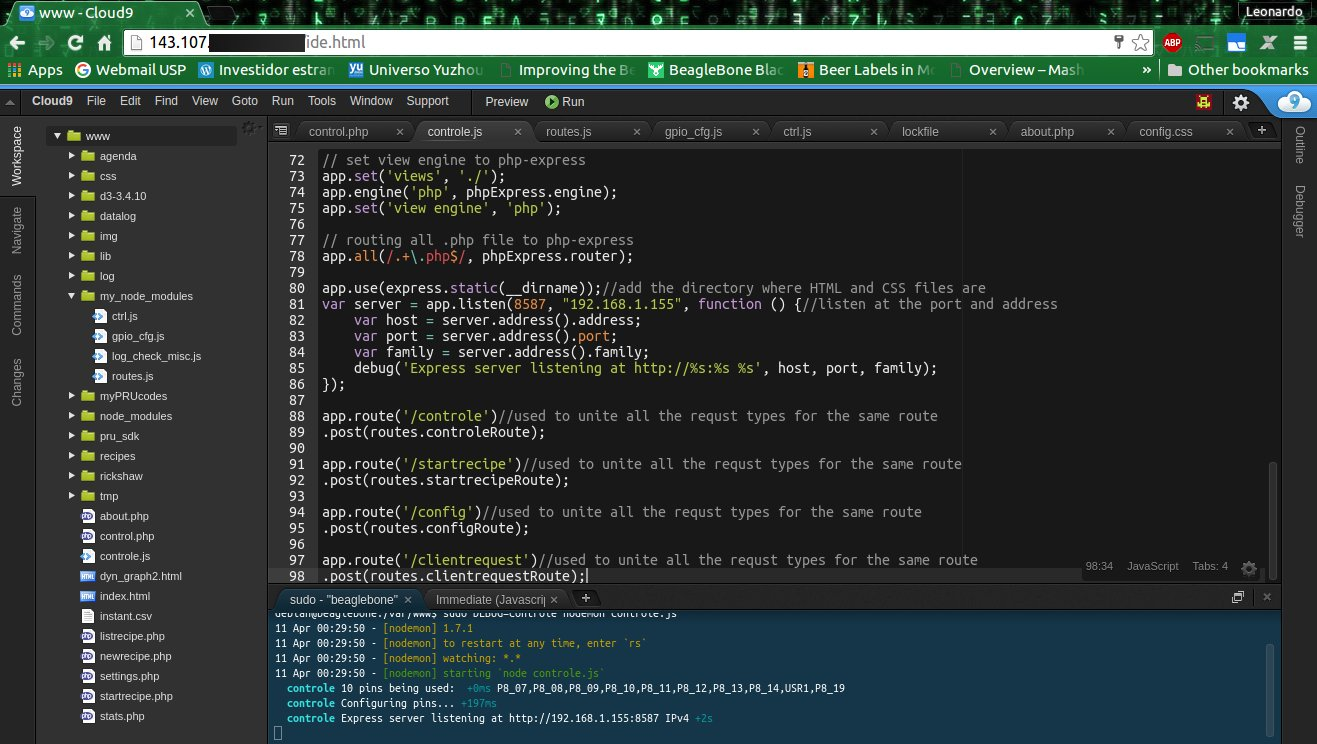
\includegraphics[scale=0.25]{./Resources/cloud9.jpg}
	\captionsetup{justification=centering}
	\caption[Ambiente completo do IDE \textit{Cloud9}]{Ambiente completo do IDE \textit{Cloud9}}
	\label{c9ide}
\end{figure}

\section{\textit{Git/GitHub}}
\label{ghb}

\textit{Git} � um sistema de controle de vers�o distribu�do (DVCS) e tamb�m � referido como um SCM (gerenciador de c�digos-fonte), ou seja, uma ferramenta cuja finalidade � gerenciar o desenvolvimento de \textit{software}. Um dos principais objetivos de um sistema como este � a documenta��o das mudan�as feitas nos arquivos do projeto ao longo do seu desenvolvimento, o que permite facilmente reverter arquivos ou mesmo o projeto inteiro para um estado anterior, comparar mudan�as em fun��o do tempo, verificar quem foi a �ltima pessoa a modificar um arquivo e possivelmente introduzir um bug, dentre outros recursos. E o mais importante, executar todas estas fun��es de maneira leve no que diz respeito a recursos computacionais e f�cil do ponto de vista do usu�rio \cite{git_book}.

Esta ferramenta foi escolhida dentre muitas outras DVCS dispon�veis por ser de c�digo-aberto e extremamente popular, n�o somente pelas suas qualidades mas tamb�m pelo fato de ser a DCVS usada para o controle de vers�o do Kernel do Linux, sendo que o \textit{Git} foi criado pela pr�pria comunidade de manuten��o do Kernel, incluindo Linus Torvalds \cite{git_book}. Embora a refer�ncia bibliogr�fica consultada sobre este assunto possua mais de 500 p�ginas, demonstrando o n�vel de complexidade que a ferramenta pode atingir, neste projeto somente o essencial ser� abordado --- o que significa compreender o uso de alguns comandos b�sicos.

Com rela��o ao \textit{GitHub}, este nada mais � do que um servi�o de hospedagem de reposit�rios \textit{Git}. Uma de suas grandes vantagens � a popularidade, o que o faz ser uma fonte repleta de recursos de c�digo-aberto. No que diz respeito a este trabalho, dentre suas vantagens est�o o fato de o servi�o facilitar o processo de \textit{backup} de todo o desenvolvimento realizado no �mbito de \textit{software}, prover uma estrutura que permite a replica��o do projeto com poucos comandos e tamb�m o uso deste servi�o para a reda��o da presente monografia sem a preocupa��o de ter que levar os arquivos fisicamente a diversas localidades ou depender de servi�os de armazenamento de prop�sito geral, que n�o apresentam as vantagens de um DVCS.

Para configurar uma conta no \textit{Github}, o primeiro passo foi a realiza��o do cadastro em \url{https://github.com}, seguida da cria��o de um reposit�rio online, conforme ilustrado na figura \ref{gitcreate}. Ap�s isto, o reposit�rio foi clonado na BBB e os arquivos relevantes do sistema foram copiados para ele. Observe-se que esta abordagem foi improvisada devido ao fato de arquivos de configura��o, dentre outros, encontrarem-se em reposit�rios espec�ficos do sistema, j� que o mais adequado seria que todos os arquivos do projeto fossem criados na pasta do \textit{Git}. Para instalar, configurar o \textit{Git} e clonar o reposit�rio rec�m criado do \textit{GitHub} para a BBB, foram executados os comandos descritos na caixa de c�digo-fonte \ref{install_git}.

\begin{figure}[H]
	\centering
	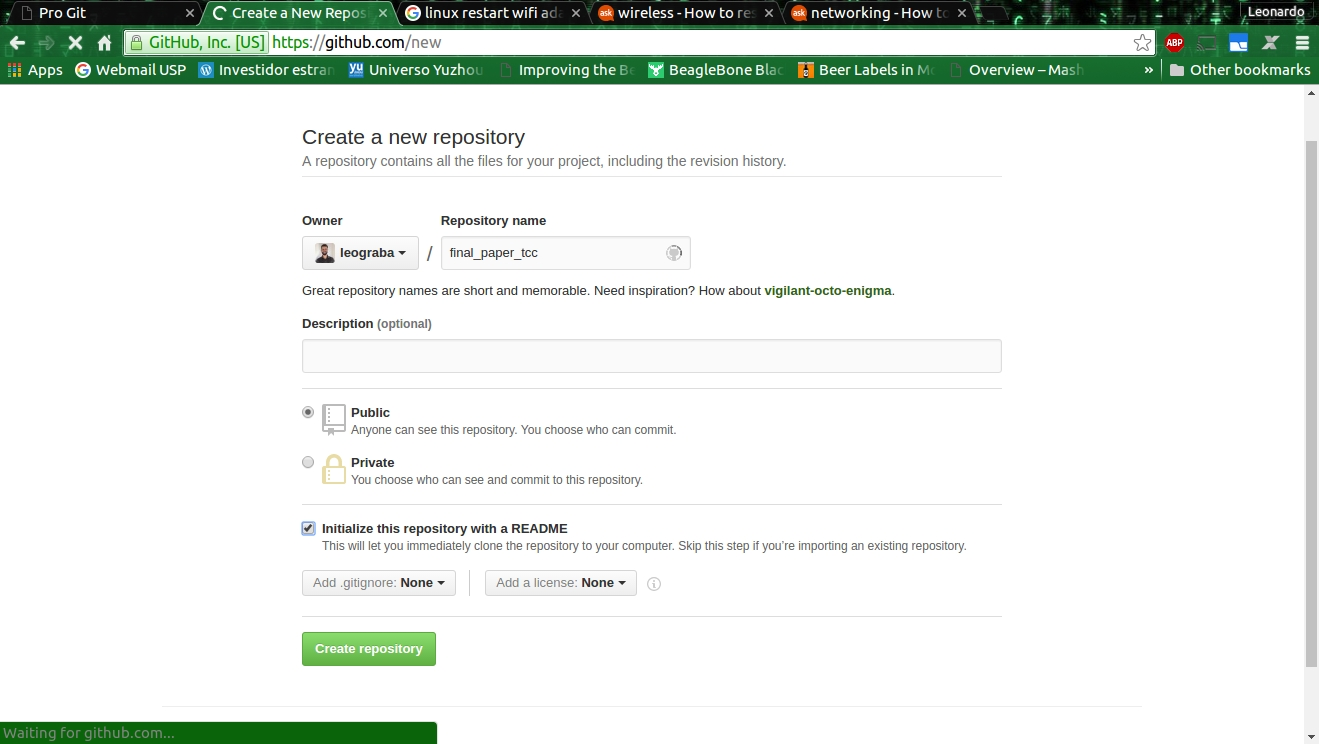
\includegraphics[scale=0.30]{./Resources/git-repo-creation.jpg}
	\captionsetup{justification=centering}
	\caption[Cria��o de reposit�rio no \textit{GitHub}]{Cria��o de reposit�rio no \textit{GitHub}}
	\label{gitcreate}
\end{figure}

\lstset{language=bash}
\begin{lstlisting}[frame=single, basicstyle=\linespread{0.85}\ttfamily, caption=Instala��o do \textit{Git} e c�pia do reposit�rio do \textit{GitHub} para a BBB, label=install_git]
sudo apt-get install git
git configure --global user.name "Nome"
git configure --global user.email email@exemplo.com
cd ~
git clone https://github.com/leograba/final_paper_tcc.git
\end{lstlisting}

Ap�s a clonagem do diret�rio \textit{final\_paper\_tcc} do \textit{GitHub} para a BBB, todos os arquivos relevantes ao projeto foram copiados para ele e, subsequentemente, adicionados ao \textit{Git}: sempre que um arquivo � adicionado ou modificado em um reposit�rio \textit{Git}, ele � ignorado a menos que seja executado o comando \textit{git add arquivo} --- isto permite flexibilidade, principalmente com rela��o a arquivos que n�o devem ser adicionados ao reposit�rio, como arquivos auxiliares gerados por compiladores, por exemplo. Ap�s cada mudan�a, para torn�-la efetiva � preciso executar o comando \textit{git commit -m "mensagem para registro"}, que al�m da data e hora da modifica��o, permite adicionar uma mensagem para identificar o que foi modificado desde o �ltimo \textit{commit}. Por fim, foi preciso enviar as mudan�as do reposit�rio local para o \textit{GitHub}. O processo de adicionar arquivos novos/modificados, fazer \textit{commit} nas mudan�as e atualizar a origem remota est� descrito no c�digo-fonte \ref{git_commit} e foi usado sempre que mudan�as foram feitas ao projeto, desde implementa��es de funcionalidades a corre��es de \textit{bugs}. Um exemplo de \textit{commit} ap�s mudan�as incrementais � apresentado na figura \ref{commit_terminal}.

\lstset{language=bash}
\begin{lstlisting}[frame=single, basicstyle=\linespread{0.85}\ttfamily, caption=Primeiro \textit{git commit}, label=git_commit]
git add .
git commit "Primeiro commit"
git push origin master
\end{lstlisting}

\begin{figure}[H]
	\centering
	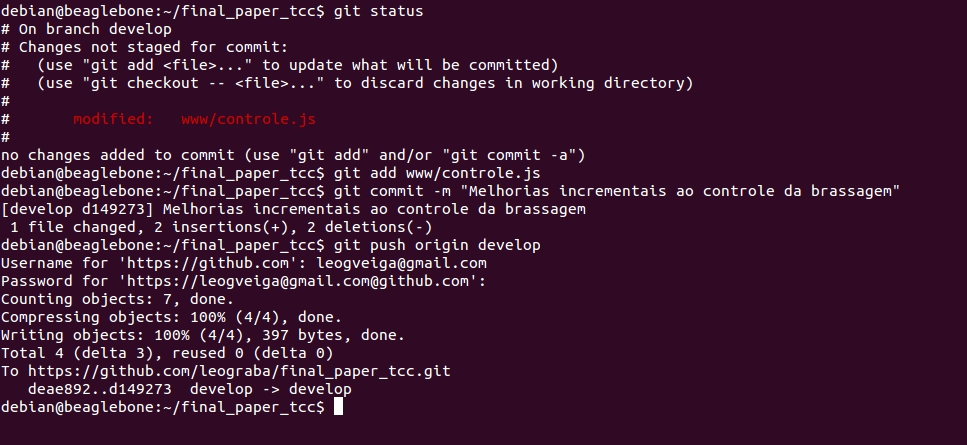
\includegraphics[scale=0.40]{./Resources/git-edit.jpg}
	\captionsetup{justification=centering}
	\caption[Fazendo \texit{git commit} ap�s mudan�as incrementais]{Fazendo \texit{git commit} ap�s mudan�as incrementais}
	\label{commit_terminal}
\end{figure}


%%%%%%%%%%%%%%%%%%%%%%%%%%%%%%%%%%%%%%%%%%%%%%%%%%%%%%%%%%%%%%%%%%%%%%%%%%

\section{Gera��o de gr�fico e registro de temperatura em Python}
Nesta se��o s�o apresentados os resultados e discuss�es referentes ao registro de temperatura em arquivo CSV e ao gr�fico gerado em Python.

\subsection{Registro de temperatura}

Na figura \ref{csv_log_example} � apresentada uma amostra de arquivo CSV gerado pelo script \ref{tlog_log}, e que valida o funcionamento da aplica��o.

\begin{figure}[H]
	\centering
	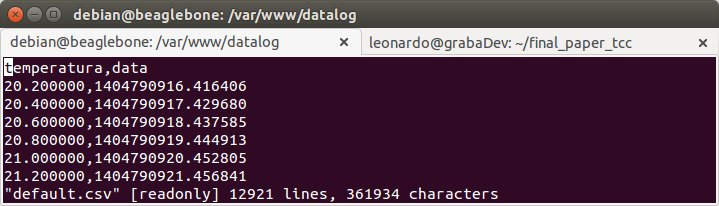
\includegraphics[scale=0.50]{./Resources/csv_log_example.jpg}
	\captionsetup{justification=centering}
	\caption[Arquivo CSV com registro de temperaturas gerado em Python]{Arquivo CSV com registro de temperaturas gerado em Python}
	\label{csv_log_example}
\end{figure}

Observa-se a partir deste que o tempo de amostragem, mesmo ap�s o estudo do ap�ndice \ref{analise_tread_temp}, tem m�dia cujo valor foi de 1,008s, diferente dos 1s desejados. Ainda assim, � preciso ressaltar que este valor est� sujeito a mudan�as em fun��o da carga do sistema, o que significa que a diferen�a de 8ms do tempo m�dio n�o seria eliminada durante a execu��o da aplica��o de controle do processo de produ��o de cerveja. Caso seja estritamente necess�rio para uma aplica��o que o tempo de amostragem n�o sofra varia��es, deve ser cogitado o uso de um sistema operacional de tempo real, do subsistema PRU-ICSS da BBB ou de um microcontrolador auxiliar que se comunique com a BBB por meio de um barramento de comunica��o.

Para confirmar o funcionamento da fun��o que faz o registro da �ltima temperatura lida em um arquivo separado, o comando \textit{tail} do Linux foi empregado. Na figura \ref{log_funciona} � apresentado o resultado pr�tico desta abordagem.

\begin{figure}[H]
	\centering
	\begin{subfigure}{.46\textwidth}
		\centering
		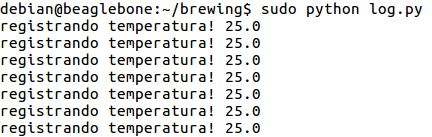
\includegraphics[height=2.2cm]{./Resources/logpy.png}
		\caption{Script python em execu��o}
		\label{log_funciona:1}
	\end{subfigure}
	\begin{subfigure}{.46\textwidth}
		\centering
		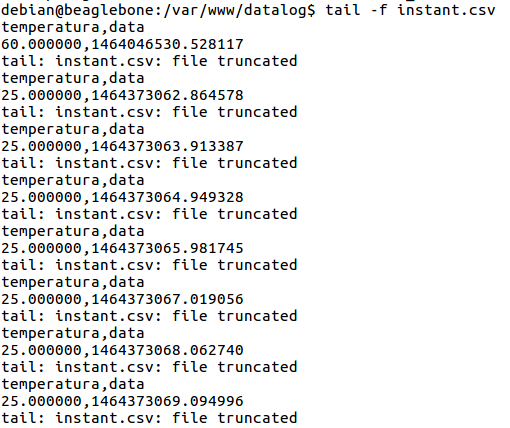
\includegraphics[height=7.2cm]{./Resources/log_tailpy.png}
		\caption{Arquivo de registro da �ltima temperatura}
		\label{log_funciona:2}
	\end{subfigure}
	\captionsetup{justification=centering}
	\caption[Conformidade da atualiza��o do arquivo de registro da �ltima temperatura capturada pelo script Python]{Conformidade da atualiza��o do arquivo de registro da �ltima temperatura capturada pelo script Python}
	\label{log_funciona}
\end{figure}

\subsection{Gr�fico de temperatura}

Na figura \ref{py_graph_7200p} � apresentado um gr�fico que foi gerado na BBB a partir de 7200 pontos amostrados, ou seja, aproximadamente 120 minutos. Este tempo foi escolhido uma vez que dificilmente o cozimento do mosto ou a fervura dura mais do que isso, portanto provando que a implementa��o � fact�vel para o uso a que se destina. A tabela  \ref{tabela_tempo_graph_python} apresenta informa��es estat�sticas sobre o tempo de computa��o necess�rio para a gera��o do gr�fico. A figura \ref{amostras_graph} apresenta o processo de verifica��o do n�mero de pontos registrados e o posterior processo de coleta dos dados que deram origem � tabela \ref{tabela_tempo_graph_python}.

\begin{figure}[H]
	\centering
	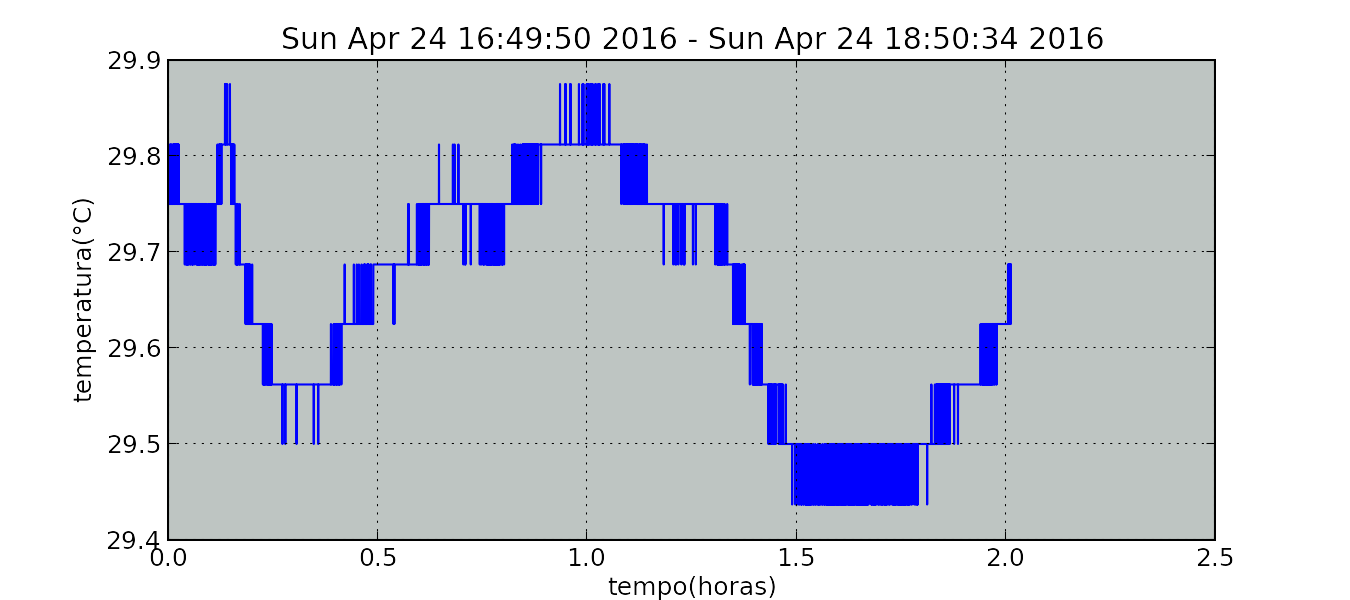
\includegraphics[scale=0.65]{./Resources/py_graph_7200p.png}
	\captionsetup{justification=centering}
	\caption[Gr�fico com 7200 pontos gerado em Python]{Gr�fico com 7200 pontos gerado em Python}
	\label{py_graph_7200p}
\end{figure}

%\begin{center}
	\begin{table}[H]
		\centering
		\captionsetup{justification=centering}
		\caption[Estat�sticas referentes ao tempo de gera��o de gr�fico na BBB, para 7200 pontos em Python]{Estat�sticas referentes ao tempo de gera��o de gr�fico na BBB, para 7200 pontos em Python}
		\label{tabela_tempo_graph_python}
		\begin{tabular}{ | M{5cm} | M{2cm} |}
			\hline
			\textbf{Descri��o} & \textbf{Valor} \\ \hline
			N.\si{\degree} de amostras & 30\\ \hline
			M�dia (s) & 2,106\\ \hline
			M�ximo (s) & 2,068\\ \hline
			M�nimo (s) & 2,149\\ \hline
			Desvio padr�o (s) & 0,023\\ \hline
		\end{tabular}
	\end{table}
%\end{center}

\begin{figure}[H]
	\centering
	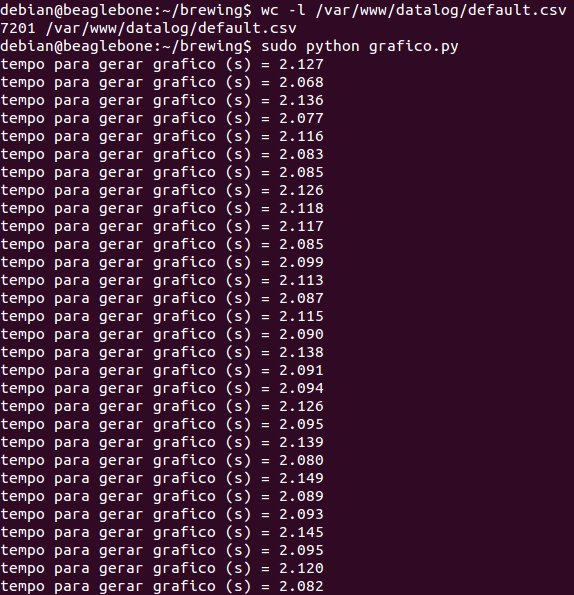
\includegraphics[scale=0.50]{./Resources/log_py_graph_7200p.jpg}
	\captionsetup{justification=centering}
	\caption[Gera��o de gr�fico em Python m�ltiplas vezes para obter o tempo m�dio]{Gera��o de gr�fico em Python m�ltiplas vezes para obter o tempo m�dio}
	\label{amostras_graph}
\end{figure}

Tamb�m foi realizado um registro de temperatura durante 38 dias ininterruptos, para comprovar a robustez da aplica��o de registro de temperatura, a capacidade de gera��o de gr�fico para um n�mero de pontos muito superior ao de uma produ��o de cerveja e tamb�m para comprova��o do funcionamento da escala ajust�vel em fun��o da logevidade do arquivo de registros. O gr�fico gerado a partir deste registro � apresentado na figura \ref{graph_long} e indica a temperatura da sa�da de ventila��o de um notebook com problemas de resfriamento.

\begin{figure}[H]
	\centering
	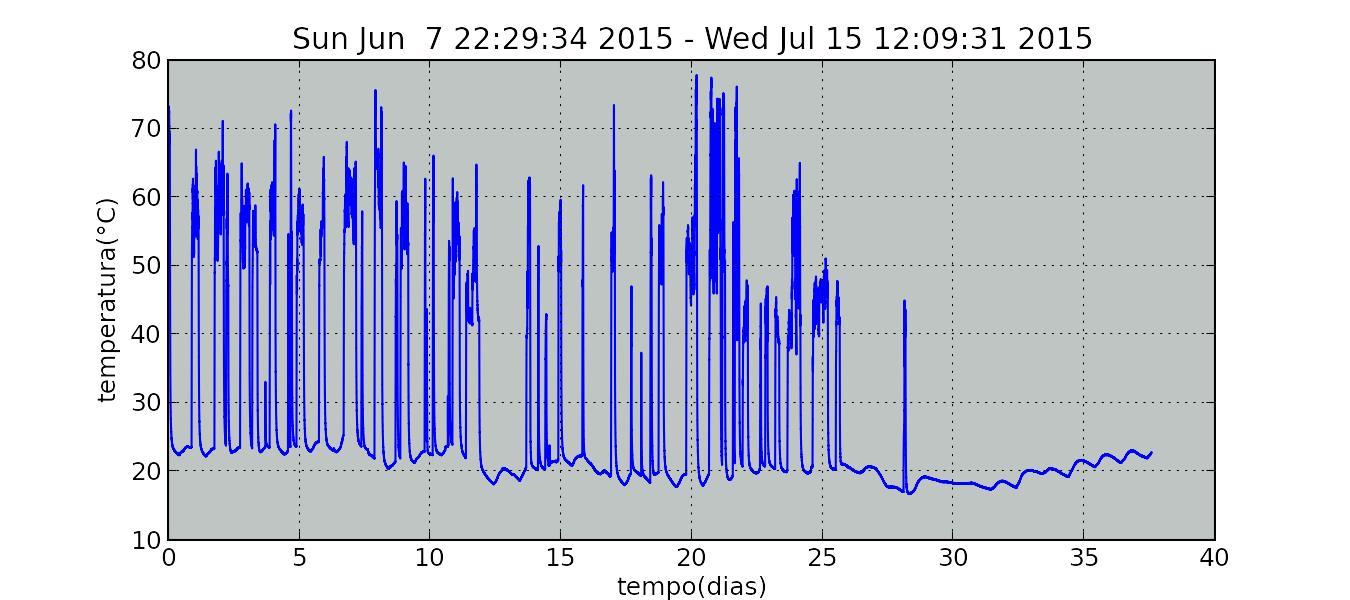
\includegraphics[scale=0.60]{./Resources/tplot.png}
	\captionsetup{justification=centering}
	\caption[Gera��o de gr�fico em Python a partir de um volume elevado de dados]{Gera��o de gr�fico em Python a partir de um volume elevado de dados}
	\label{graph_long}
\end{figure}


%%%%%%%%%%%%%%%%%%%%%%%%%%%%%%%%%%%%%%%%%%%%%%%%%%%%%%%%%%%%%%%%%%%%%%%%%%

\section{Aplica��o \textit{server-side} em Node.js}
\label{nodectrl_res}
Nesta se��o ser�o apresentados os resultados referentes � implementa��o \textit{server-side} em Node.js. Ser�o apresentados desde resultados simples, como a verifica��o da instala��o do Node, at� o resultado da simula��o do processo de controle autom�tico da brassagem.

O primeiro teste realizado, descrito na figura \ref{node_working}, demonstra que o Node.js foi corretamente instalado.

\begin{figure}[H]
	\centering
	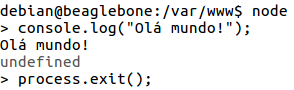
\includegraphics[scale=0.65]{./Resources/node_working.png}
	\captionsetup{justification=centering}
	\caption[Teste de funcionamento do Node.js]{Teste de funcionamento do Node.js}
	\label{node_working}
\end{figure}

\subsection{Acesso a GPIO e PWM}

O teste de funcionamento do acesso a GPIO foi realizado por meio de chamadas peri�dicas � fun��o \textit{testIO} descrita na se��o \ref{gpio_sec}. Uma vez que esta fun��o chaveia 9 pinos, sendo que somente um deles fica em n�vel alto por vez, as observa��es em bancada foram realizadas com dois pinos consecutivos, dada a limita��o de 2 canais do oscilosc�pio. 

O resultado de um teste preliminar, resultante da observa��o em bancada para o chaveamento destes pinos, � apresentado na figura \ref{gpio_sw}. Neste teste preliminar, foram coletados dados relativos somente a uma amostra.

\begin{figure}[H]
	\centering
	\begin{subfigure}{.46\textwidth}
		\centering
		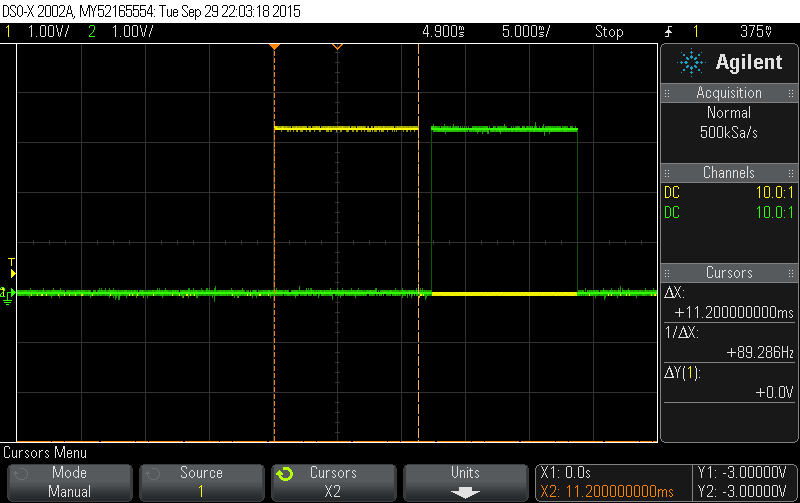
\includegraphics[height=4.5cm]{./Resources/BonescriptIO/high-10ms-9bits/scope_1.png}
		\caption{Tempo em n�vel alto do canal 1 (amarelo)}
		\label{gpio_sw:1}
	\end{subfigure}
	\begin{subfigure}{.46\textwidth}
		\centering
		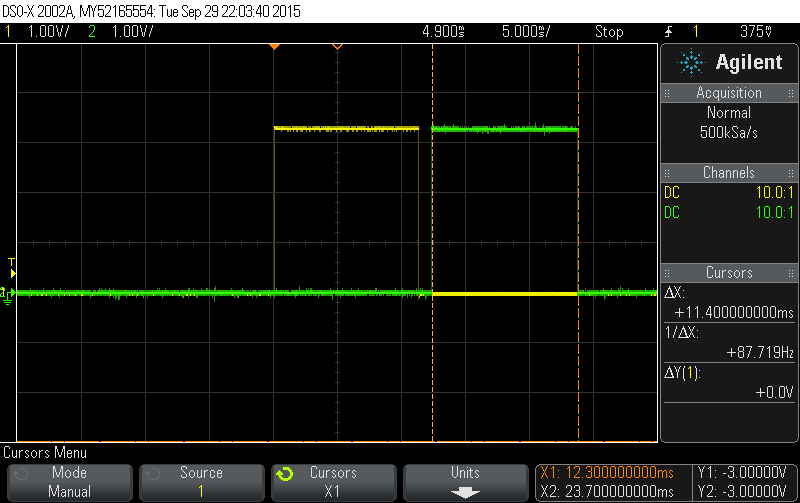
\includegraphics[height=4.5cm]{./Resources/BonescriptIO/high-10ms-9bits/scope_2.png}
		\caption{Tempo em n�vel alto do canal 2 (verde)}
		\label{gpio_sw:2}
	\end{subfigure}
	\begin{subfigure}{.65\textwidth}
		\centering
		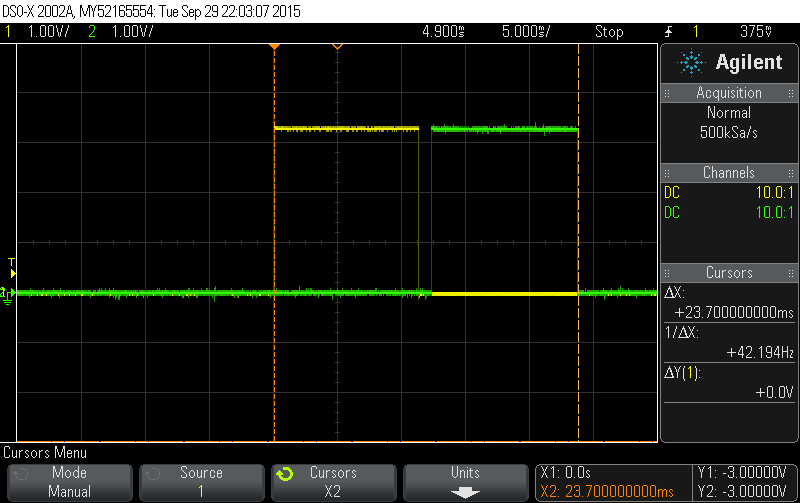
\includegraphics[height=6cm]{./Resources/BonescriptIO/high-10ms-9bits/scope_0.png}
		\caption{Tempo total de chaveamento}
		\label{gpio_sw:3}
	\end{subfigure}
	\captionsetup{justification=centering}
	\caption[Observa��o do chaveamento de dois pinos de GPIO consecutivos com tempo em n�vel alto esperado de 10ms]{Observa��o do chaveamento de dois pinos de GPIO consecutivos com tempo em n�vel alto esperado de 10ms}
	\label{gpio_sw}
\end{figure}

A partir desta coleta de dados, obt�m-se os valores de tempo m�dio em n�vel alto, tempo inativo entre chaveamentos e erro de tempo em n�vel alto, todos para somente um ciclo de amostragem. Os valores est�o descritos na tabela \ref{um_ciclo_gpio}.

\begin{table}[H]
	\centering
	\captionsetup{justification=centering}
	\caption[Estat�sticas referentes ao tempo de um �nico chaveamento de GPIO usando o m�dulo \textit{gpio\_config} em Node.js]{Estat�sticas referentes ao tempo de um �nico chaveamento de GPIO usando o m�dulo \textit{gpio\_config} em Node.js}
	\label{um_ciclo_gpio}
	\begin{tabular}{ | M{7.5cm} | M{2cm} |}
		\hline
		\textbf{Descri��o} & \textbf{Valor (ms)} \\ \hline
		Tempo m�dio esperado em n�vel alto & 10,0\\ \hline
		Tempo m�dio medido em n�vel alto & 11,3\\ \hline
		Tempo inativo entre chaveamentos & 1,1\\ \hline
		Erro de tempo em n�vel alto (\%) & 13,0\\ \hline
	\end{tabular}
\end{table}

Foi notado tamb�m que a carga de processamento exigida da CPU � de 20\%, valor n�o desprez�vel. Este resultado est� documentado na figura \ref{cpu_intensive}.

\begin{figure}[H]
	\centering
	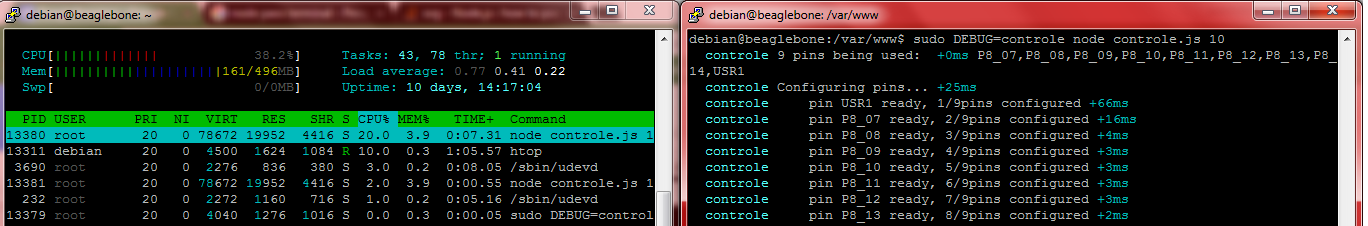
\includegraphics[scale=0.40]{./Resources/BonescriptIO/high-10ms-9bits/Carga_processo.png}
	\captionsetup{justification=centering}
	\caption[Carga da CPU dedicada ao chaveamento de GPIO em Node.js com tempo de chaveamento de 10ms]{Carga da CPU dedicada ao chaveamento de GPIO em Node.js com tempo de chaveamento de 10ms}
	\label{cpu_intensive}
\end{figure}

Observados os valores do teste preliminar, nos quais tanto o tempo de chaveamento, que idealmente deveria ser nulo, quanto o tempo em n�vel alto, que apresentou erro de 13\% n�o foram desprez�veis, foi decidido realizar um estudo mais completo do acesso a GPIO, medindo n�o somente temporiza��o quanto uso de CPU pelo processo. Para isto foram definidos tempos em n�vel alto desde 0,1ms at� 500ms e foram coletadas 30 amostras para cada situa��o. Os dados consolidados s�o apresentados na tabela \ref{gpio_consolidados}.

\begin{table}[H]
	\centering
	\captionsetup{justification=centering}
	\caption[Estat�sticas referentes ao chaveamento de GPIO usando o m�dulo \textit{gpio\_config} em Node.js]{Estat�sticas referentes ao chaveamento de GPIO usando o m�dulo \textit{gpio\_config} em Node.js}
	\label{gpio_consolidados}
	\begin{tabular}{ | M{1.9cm} | M{1.9cm} | M{1.9cm} | M{1.9cm} | M{1.9cm} | M{1.9cm} | M{1.9cm} |}
		\hline
		\textbf{Tempo esperado em n�vel alto(ms)} & \textbf{Tempo m�dio em n�vel alto (ms)} & \textbf{Tempo m�nimo em n�vel alto} & \textbf{Tempo m�ximo em n�vel alto} & \textbf{Desvio padr�o (ms)} & \textbf{Erro (\%)} & \textbf{Carga da CPU (\%)}\\ \hline
		0,1 & 1,89 & 1,69 & 3,83 & 0,40 & 1793,21 & 56 \\ \hline
		0,2 & 1,81 & 1,57 & 2,73 & 0,22 & 806,71 & 56\\ \hline
		0,5 & 1,84 & 1,68 & 3,62 & 0,34 & 268,09 & 56\\ \hline
		1,0 & 1,85 & 0,45 & 3,79 & 0,51 & 85,10 & 56\\ \hline
		1,5 & 2,69 & 2,16 & 4,69 & 0,49 & 79,40 & 60\\ \hline
		2,0 & 2,77 & 1,88 & 3,81 & 0,26 & 38,45 & 38\\ \hline
		2,5 & 3,51 & 2,92 & 3,85 & 0,17 & 40,34 & 46\\ \hline
		3,0 & 4,29 & 3,50 & 6,00 & 0,44 & 43,08 & 43\\ \hline
		4,9 & 5,80 & 4,58 & 6,80 & 0,50 & 18,28 & 43\\ \hline
		5,0 & 6,37 & 5,53 & 8,13 & 0,44 & 27,36 & 31\\ \hline
		5,1 & 6,68 & 5,60 & 8,33 & 0,63 & 30,94 & 33\\ \hline
		10,0 & 11,46 & 10,55 & 12,51 & 0,37 & 14,58 & 21\\ \hline
		20,0 & 21,71 & 21,34 & 23,07 & 0,38 & 8,57 & 12\\ \hline
		50,0 & 51,74 & 50,62 & 54,68 & 0,71 & 3,47 & 10\\ \hline
		100,0 & 102,08 & 100,76 & 104,04 & 0,57 & 2,08 & 10\\ \hline
		500,0 & 502,41 & 501,40 & 503,40 & 0,37 & 0,50 & 10\\ \hline
	\end{tabular}
\end{table}

A partir destes dados, foi observado que a t�cnica de chaveamento de GPIO em Node.js apresentou erro acima de 5\% at� para valores entre 20ms e 50ms, o que desqualifica o uso desta t�cnica em situa��es nas quais temporiza��o � cr�tica. Para valores abaixo de 10ms, o erro superior a 30\% torna esta t�cnica invi�vel mesmo para aplica��es nas quais a toler�ncia � alta. Observou-se que o limite m�dio inferior de chaveamento ficou na ordem de 1,8ms e foi alcan�ado somente para tempos esperados iguais ou menores do que 1,0ms.

Outra informa��o obtida a partir da tabela \ref{gpio_consolidados} � o fato de que o tempo de chaveamento n�o foi limitado pelo uso da CPU. Da figura \ref{cpu_intensive} nota-se que 18\% da carga da CPU estava sendo requisitada pelas outras tarefas da BBB e, portanto, mesmo para o pior caso de chaveamento observado, com uso de 60\%, ainda assim, havia poder de processamento ocioso.

Quanto ao PWM, foi verificado o seu funcionamento para a frequ�ncia de f=50Hz, ou seja, a mesma frequ�ncia necess�ria para opera��o do servo-motor, e ciclo de trabalho de 50\%. O resultado est� exposto na figura \ref{pwm_teste}. Resultados complementares a este s�o apresentados na se��o \ref{circuitos_res}, que aborda especificamente os resultados do servo-motor, mas que est� intr�nsecamente ligada ao bom funcionamento do PWM.

\begin{figure}[H]
	\centering
	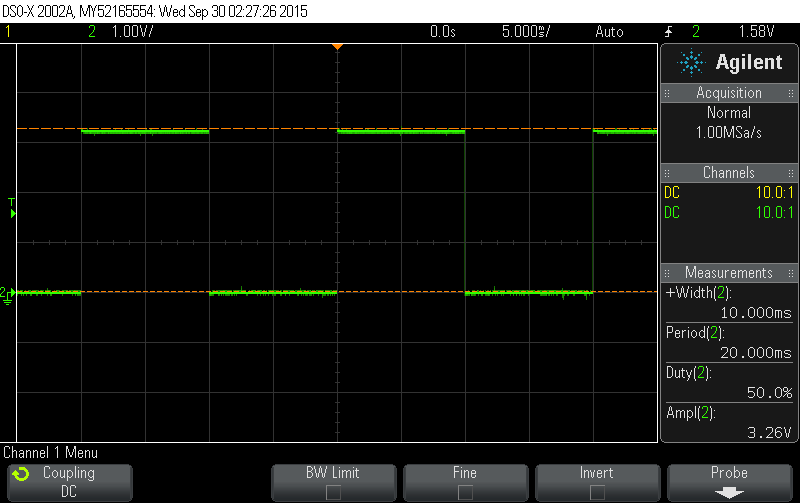
\includegraphics[scale=0.45]{./Resources/BonescriptIO/PWM-servo-motor/pwm__________1.png}
	\captionsetup{justification=centering}
	\caption[Verifica��o de funcionamento do PWM configurado por meio do Node.js, com f=50Hz e \textit{duty-cycle}=50\%]{Verifica��o de funcionamento do PWM configurado por meio do Node.js, com f=50Hz e \textit{duty-cycle}=50\%}
	\label{pwm_teste}
\end{figure}

\subsection{Servidor Express}

Como o objetivo do servidor implementado neste trabalho foi exclusivamente o de servir conte�do via web e proporcinar a base para a interface de usu�rio, o cap�tulo de resultados \ref{resIntUser}, que apresenta os resultados referentes � interface gr�fica de usu�rio, � um resultado direto do sucesso da implementa��o utilizando o \textit{framework} Express.

N�o obstante, foi observado que a execu��o da aplica��o completa em Node.js, quando o sistema fica ocioso, ocupa 8,1\% dos recursos de mem�ria da BBB, ou seja 40Mb de um total de 496Mb. Quanto aos recursos de processamento, o \textit{software} de monitoramento de recursos \textit{htop} oscila entre 0\% e 1\% de uso da CPU para esta tarefa.

Para observar a carga do sistema e comprovar o embasamento te�rico exposto no cap�tulo \ref{node_js_sec}, que indica que o uso de Node.js � apropriado para opera��es de I/O intensivo, foi observado o consumo de recursos da aplica��o com um n�mero variado de abas de internet abertas ao mesmo tempo na interface de controle manual do sistema. A escolha desta p�gina como \textit{benchmark} deriva-se do fato de que ela se comunica com o servidor a cada 0,5s. Os resultados do teste se encontram na tabela \ref{bench_server}.

\begin{table}[H]
	\centering
	\captionsetup{justification=centering}
	\caption[Consumo de recursos de mem�ria e CPU da aplica��o em fun��o do n�mero de clientes conectados � BBB]{Consumo de recursos de mem�ria e CPU da aplica��o em fun��o do n�mero de clientes conectados � BBB}
	\label{bench_server}
	\begin{tabular}{ | M{5cm} | M{3cm} | M{3cm} |}
		\hline
		\textbf{$N^o$ de abas} & \textbf{Mem�ria RAM (\%)} & \textbf{Faixa de consumo da CPU (\%)}\\ \hline
		1 & 8,7 & 2 - 6 \\ \hline
		2 & 8,8 &  4 - 7\\ \hline
		5 & 9,0 & 6 - 12 \\ \hline
		10 & 9,9 & 11 - 32 \\ \hline
		25 & 10,1 & 21 - 54 \\ \hline
		50 & 10,1 & 34 - 68 \\ \hline
		75 & 10,1 & 52 - 93 \\ \hline
		100 & 10,2 & 38 - 91 \\ \hline
		125 & 10,3 & 58 - 91 \\ \hline
		200 & 10,3 & 45 - 91 \\ \hline
	\end{tabular}
\end{table}

� importante notar que, ap�s fechar todas as abas, o consumo de recursos do sistema voltou �s condi��es iniciais, al�m de que o desempenho do computador do cliente foi monitorado e, em nenhum momento, o consumo de recursos dos n�cleos de CPU ficou travado em 100\%. Outro teste realizado quando as 200 abas foram abertas, foi usar a interface de usu�rio em diversas abas aleat�rias para comprovar que esta continuava funcional, mesmo com muitas conex�es concorrentes: foi notada lentid�o em compara��o � opera��o com somente uma aba aberta, por�m a interface continuou funcional. A figura \ref{pczao_abas} apresenta o gerenciador de recursos do navegador Google Chrome e, por conseguinte, a quantidade de recursos de CPU, mem�ria RAM e rede demandados do computador do cliente com 200 abas da aplica��o abertas.

\begin{figure}[H]
	\centering
	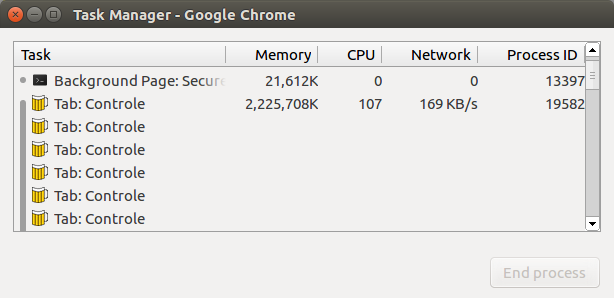
\includegraphics[scale=0.50]{./Resources/200_tabs_chrome.png}
	\captionsetup{justification=centering}
	\caption[Consumo de recursos do computador do cliente para 200 abas abertas no navegador Google Chrome]{Consumo de recursos do computador do cliente para 200 abas abertas no navegador Google Chrome}
	\label{pczao_abas}
\end{figure}

Quanto aos resultados expressos na tabela \ref{bench_server}, � importante salientar que, mesmo que o consumo m�nimo da CPU n�o tenha crescido proporcionalmente com o aumento do n�mero de abas, ainda assim � medida que este (n�mero de abas) crescia, era not�vel que a CPU passava cada vez mais tempo em n�veis mais elevados de processamento.

� importante salientar que testes no �mbito de seguran�a n�o foram conduzidos, embora este seja um t�pico de grande interesse na �rea de IoT (internet das coisas). Nota-se tamb�m que nenhuma restri��o de acesso � interface gr�fica de usu�rio foi implementada neste projeto.

\subsection{Registros e verifica��es em geral}

O m�dulo de registros e verifica��es em geral, conforme descrito na se��o \ref{registros_sec}, tem fun��es para controlar o registro de temperatura, ler o �ltimo valor registrado de temperatura, verificar a integridade de uma receita, responder para o cliente o nome de todas as receitas cadastradas no servidor e registrar o processo de brassagem. Esta se��o � dedicada a apresentar somente resultados parciais do controle do registro de brassagem e resultados do registro do processo de brassagem, uma vez que a grande maioria destas fun��es tem seus resultados descritos nas se��es \ref{temp_py_res} (registro de temperatura em Python) e \ref{resIntUser} (interface gr�fica de usu�rio).

Com rela��o ao controle do registro de temperaturas, a �nica observa��o aqui apresentada � que o arquivo de registros foi corretamente criado tanto durante as simula��es do controle da brassagem quanto durante os testes de automa��o da parte mec�nica. Isto implica que as fun��es que iniciam e param o script Python a partir do Node cumprem o seu objetivo.

Quanto ao registro do processo de brassagem, guardado no arquivo \textit{backup.log}, ap�s a simula��o da receita descrita na se��o \ref{simulacao_controle}, verificou-se que foi gerado um arquivo com 249 registros e que neste todos os c�digos de brassagem da tabela \ref{significados_log} foram encontrados ao menos em uma linha de registro. A figura \ref{registro_c9} apresenta o in�cio e o final do arquivo, acessado por meio da IDE online \textit{Cloud9}, tanto para motivo de ilustra��o quanto comprova��o da cria��o bem sucedida do registro. A tabela \ref{linhas_importantes} apresenta os campos \textit{c�digo, msg} e  \textit{timestamps:curr)} dos registros de situa��es not�veis, conforme descrito na se��o \ref{registros_sec}, e importantes da brassagem.

\begin{figure}[H]
	\centering
	\begin{subfigure}{.46\textwidth}
		\centering
		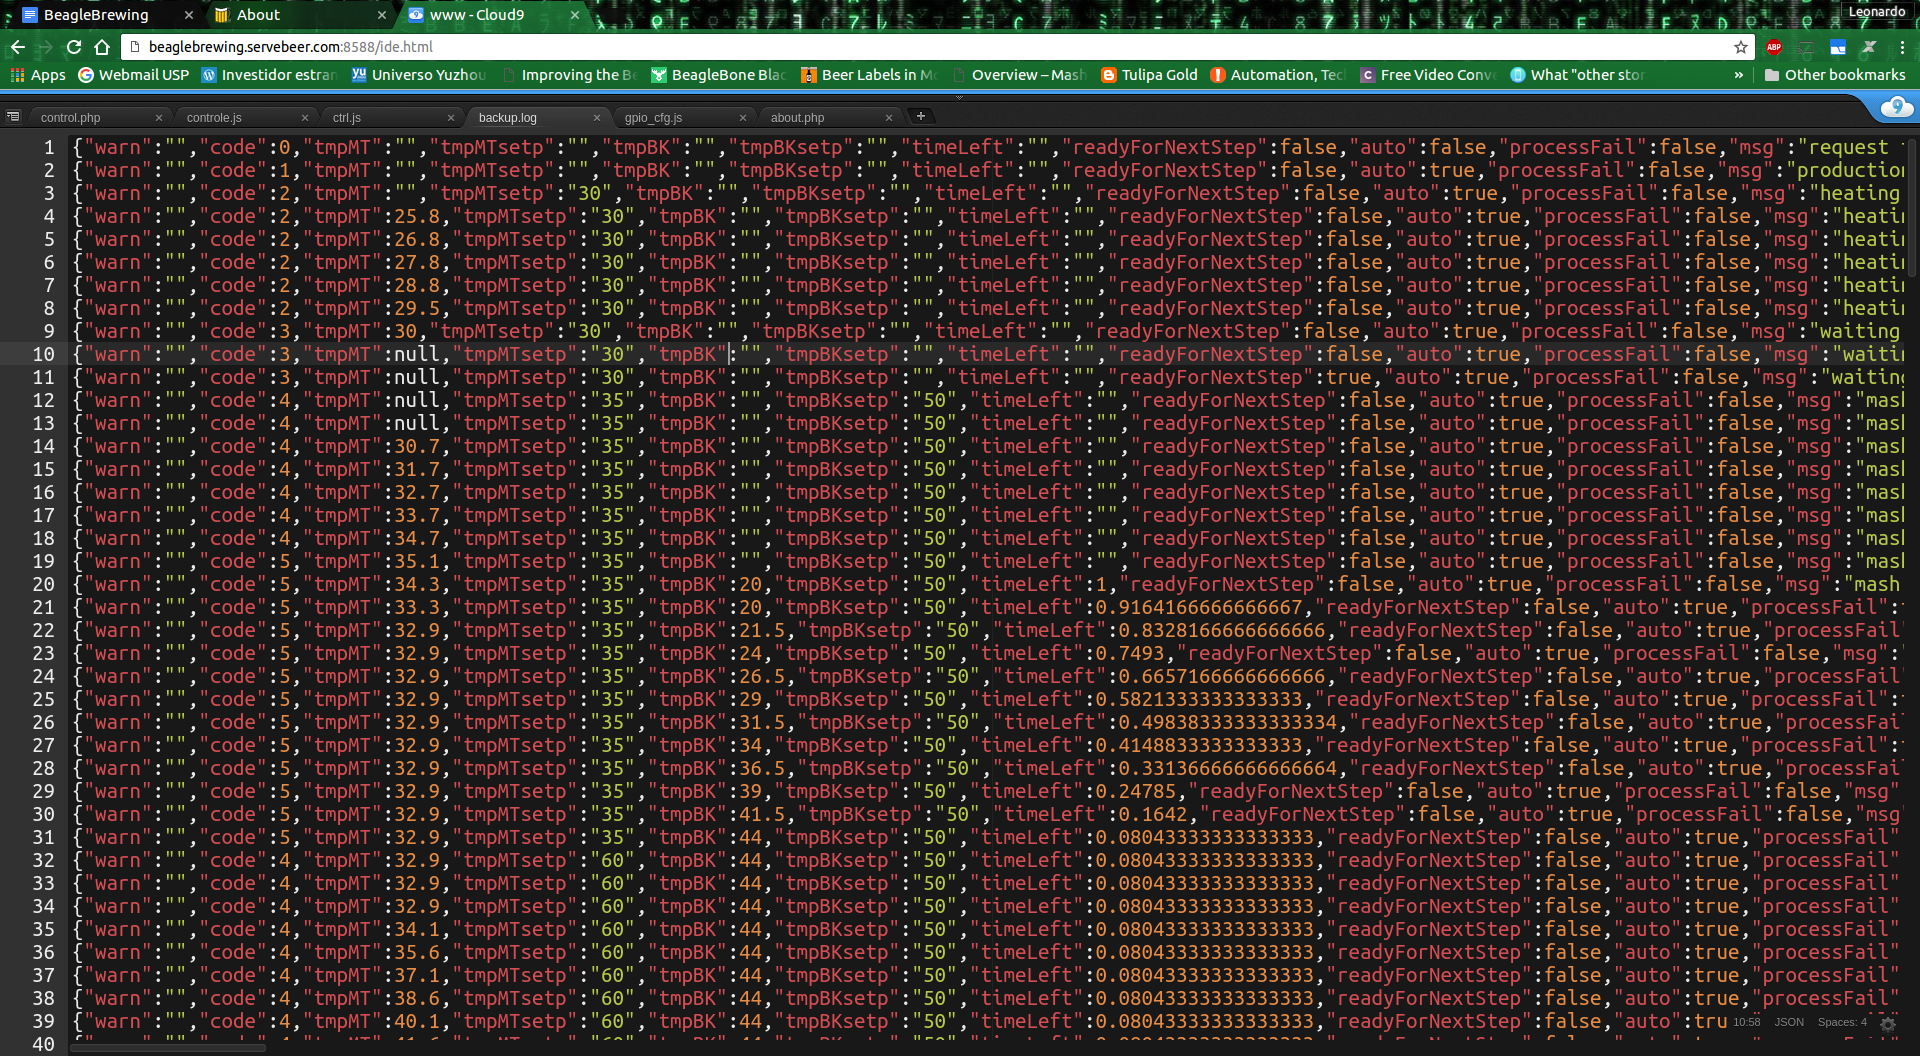
\includegraphics[height=4.5cm]{./Resources/inicio_log.png}
		\caption{Registros iniciais}
		\label{registro_c9:1}
	\end{subfigure}
	\begin{subfigure}{.46\textwidth}
		\centering
		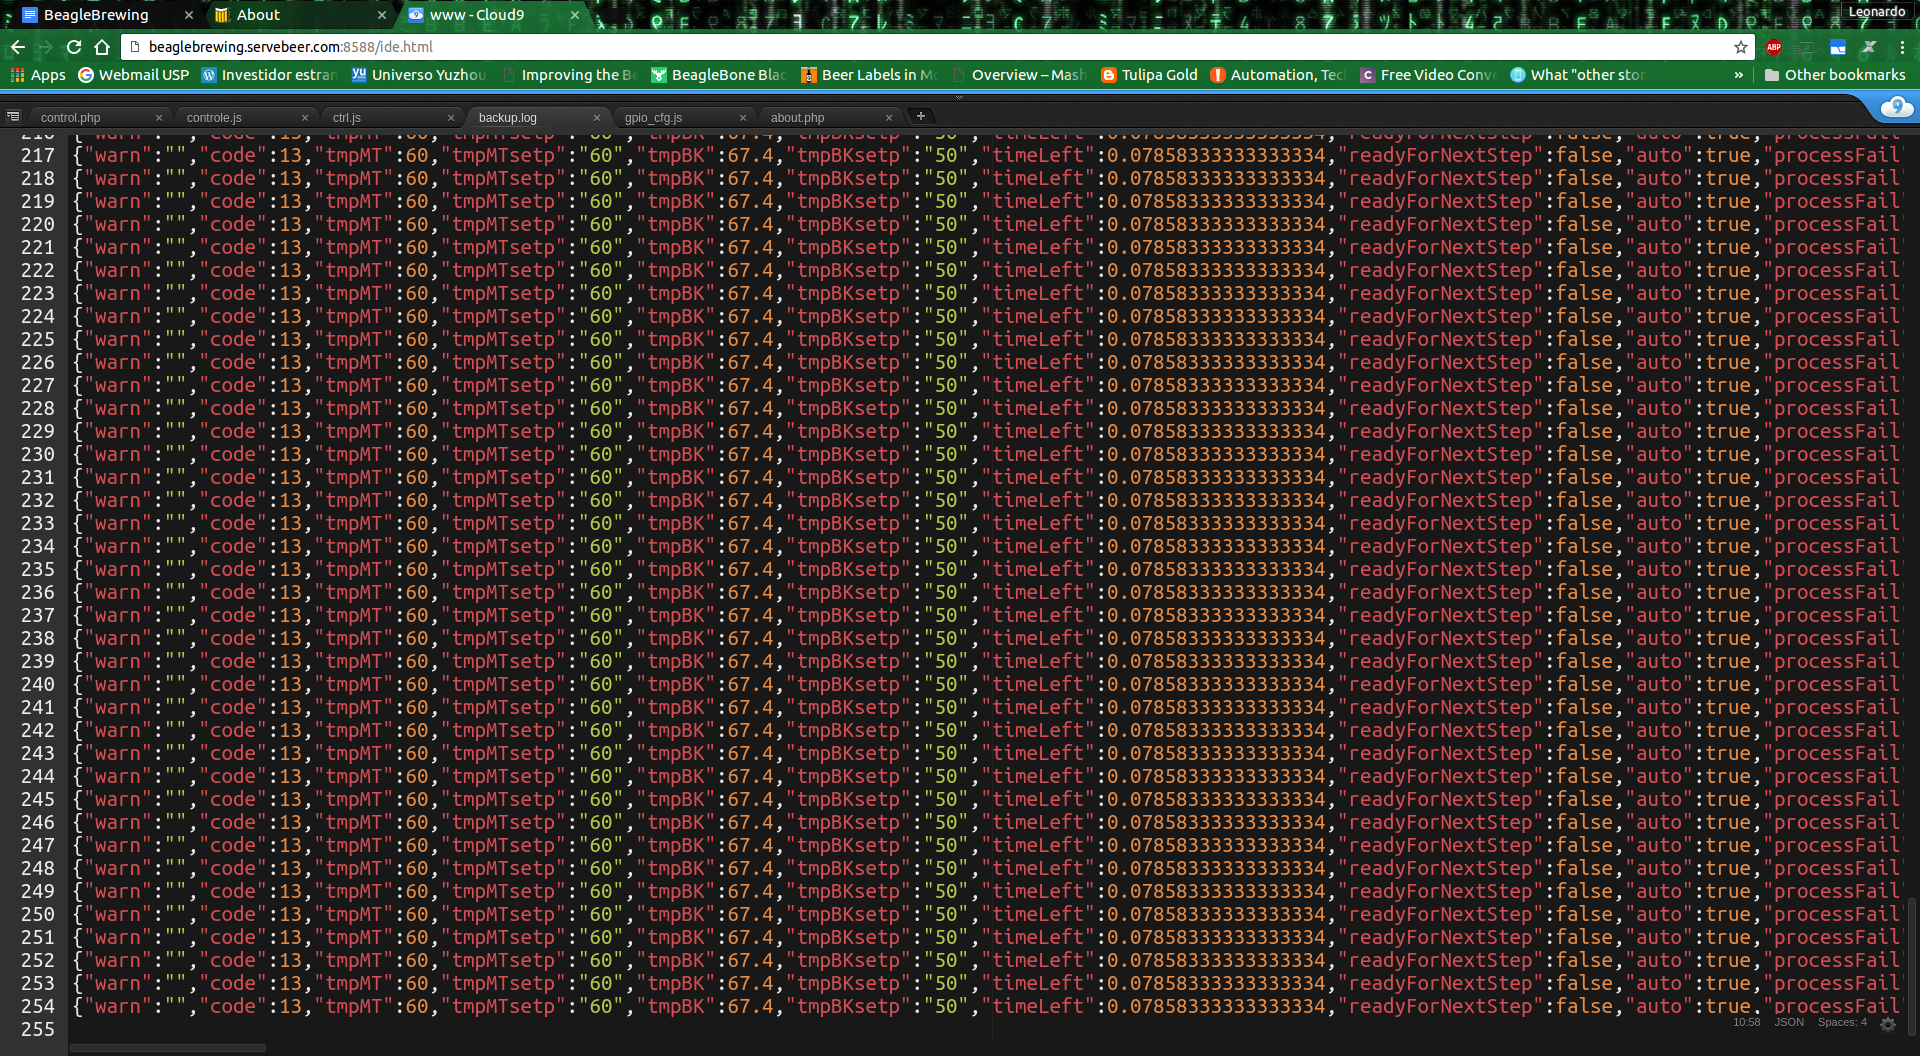
\includegraphics[height=4.5cm]{./Resources/final_log.png}
		\caption{Registros finais}
		\label{registro_c9:2}
	\end{subfigure}
	\captionsetup{justification=centering}
	\caption[Arquivo de registro do processo de brassagem]{Arquivo de registro do processo de brassagem}
	\label{registro_c9}
\end{figure}

\begin{table}[H]
	\centering
	\captionsetup{justification=centering}
	\caption[Apresenta��o dos campos \textit{c�digo, msg} e  \textit{timestamps:curr)} convertida de \textit{epoch time} para data/hora, das situa��es not�veis e importantes da brassagem]{Apresenta��o dos campos \textit{c�digo, msg} e  \textit{timestamps:curr)} (timestamp no momento do log) convertida de \textit{epoch time} para data/hora, das situa��es not�veis e importantes da brassagem}
	\label{linhas_importantes}
	\begin{tabular}{ | M{1.5cm} | M{1.5cm} | M{5cm} | M{4cm} | M{1.5cm} |}
		\hline
		\textbf{Linha} & \textbf{C�digo} & \textbf{Mensagem} & \textbf{Timestamp (UTC-3)} & Not�vel\\ \hline
		1 & 0 & request to start production & 23-05-2016 20:21:26 & sim \\ \hline
		2 & 1 & production starting & 23-05-2016 20:21:32 & n�o \\ \hline
		3 & 2 & heating mash water & 23-05-2016 20:21:32 & sim \\ \hline
		9 & 3 & waiting for grains & 23-05-2016 20:22:01 & sim \\ \hline
		12 & 4 & mash ramp in progress & 23-05-2016 20:22:13 & sim \\ \hline
		19 & 5 & mash step[1] in progress & 23-05-2016 20:22:44 & sim \\ \hline
		32 & 4 & mash ramp in progress & 23-05-2016 20:23:46 & sim \\ \hline 
		60 & 5 & mash step[2] in progress & 23-05-2016 20:26:03 & sim \\ \hline
		74 & 6 & sparging in progress & 23-05-2016 20:27:11 & sim \\ \hline
		78 & 7 & mash tun overflow & 23-05-2016 20:27:31 & n�o\\ \hline 
		84 & 6 & sparging in progress & 23-05-2016 20:28:01 & n�o \\ \hline
		126 & 8 & heating wort to boil & 23-05-2016 20:31:29 & sim \\ \hline
		127 & 9 & boiling wort & 23-05-2016 20:31:30 & sim \\ \hline
		139 & 10 & added hop [0] & 23-05-2016 20:32:30 & sim \\ \hline
		152 & 10 & added hop [2] & 23-05-2016 20:33:30 & sim \\ \hline
		165 & 10 & added hop [1] & 23-05-2016 20:34:30 & sim \\ \hline
		179 & 11 & chilling the wort & 23-05-2016 20:35:31 & sim \\ \hline
		203 & 12 & chill finished - brewing finished & 23-05-2016 20:37:32 & sim \\ \hline
		207 & 13 & cleaning recirculation & 23-05-2016 20:37:47 & sim \\ \hline
		254 & 13 & cleaning recirculation & 23-05-2016 20:41:42 & n�o \\ \hline
	\end{tabular}
\end{table}

\subsection{Simula��o do controle do processo de brassagem}

Para simular o controle do processo de brassagem, foi iniciada a receita de \textit{debug} descrita na se��o \ref{simulacao_controle} a partir da GUI e observado o comportamento tanto desta quanto das mensagens de \textit{debug} impressas pela aplica��o no terminal. A depura��o de todos os m�dulos escritos para esta aplica��o foi ativada e, inicialmente, nenhum \textit{hardware} foi ligado � BBB. As figuras \ref{console_sim_1} e \ref{console_sim_2} apresentam excertos relevantes do conjunto de mensagens impresso no terminal.

\begin{figure}[H]
	\centering
	\begin{subfigure}{.46\textwidth}
		\centering
		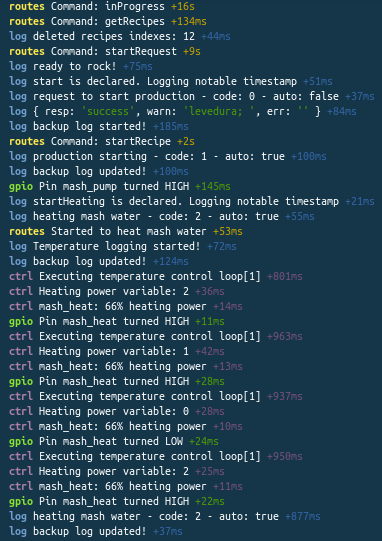
\includegraphics[height=8cm]{./Resources/simBrewing/simlog1.png}
		\caption{Acesso � GUI e in�cio da brassagem}
		\label{console_sim_1:1}
	\end{subfigure}
	\begin{subfigure}{.46\textwidth}
		\centering
		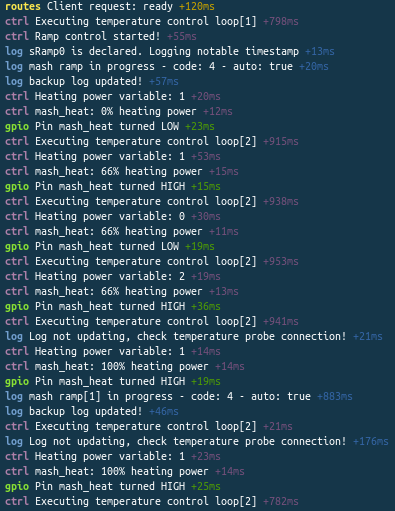
\includegraphics[height=8cm]{./Resources/simBrewing/simlog2.png}
		\caption{In�cio do controle de temperatura}
		\label{console_sim_1:2}
	\end{subfigure}
	\begin{subfigure}{.46\textwidth}
		\centering
		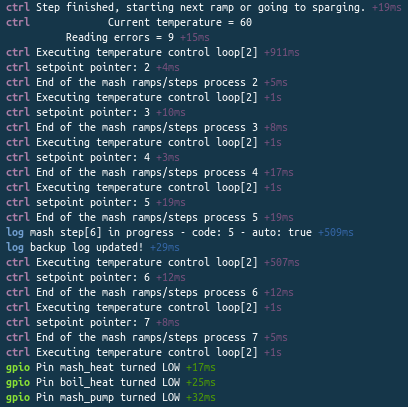
\includegraphics[height=8cm]{./Resources/simBrewing/simlog3.png}
		\caption{Final do controle de temperatura}
		\label{console_sim_1:3}
	\end{subfigure}
	\begin{subfigure}{.46\textwidth}
		\centering
		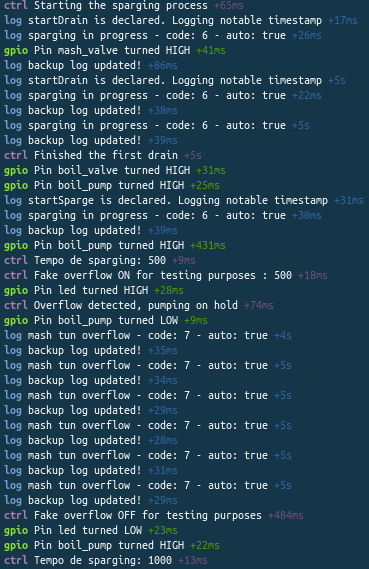
\includegraphics[height=8cm]{./Resources/simBrewing/simlog4.png}
		\caption{In�cio da lavagem dos gr�os (\textit{sparging})}
		\label{console_sim_1:4}
	\end{subfigure}
	\captionsetup{justification=centering}
	\caption[Excertos relevantes das mensagens de depura��o do processo de simula��o da brassagem (parte 1)]{Excertos relevantes das mensagens de depura��o do processo de simula��o da brassagem (parte 1)}
	\label{console_sim_1}
\end{figure}

\begin{figure}[H]
	\centering
	\begin{subfigure}{.46\textwidth}
		\centering
		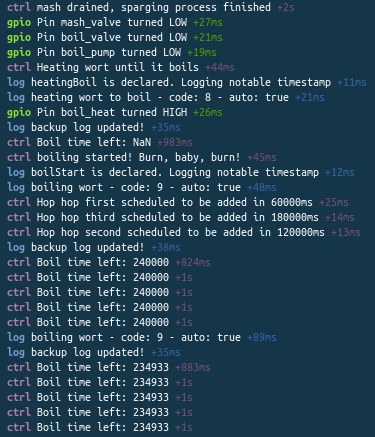
\includegraphics[height=7.5cm]{./Resources/simBrewing/simlog5.png}
		\caption{In�cio da fervura do mosto}
		\label{console_sim_2:1}
	\end{subfigure}
	\begin{subfigure}{.46\textwidth}
		\centering
		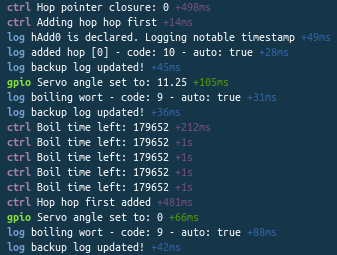
\includegraphics[height=5.2cm]{./Resources/simBrewing/simlog6.png}
		\caption{Adi��o de l�pulo � panela de fervura}
		\label{console_sim_2:2}
	\end{subfigure}
	\begin{subfigure}{.46\textwidth}
		\centering
		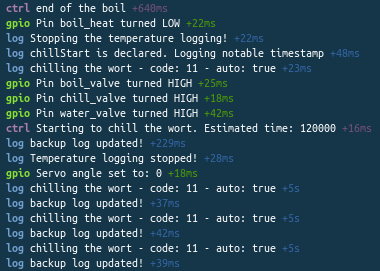
\includegraphics[height=5.0cm]{./Resources/simBrewing/simlog7.png}
		\caption{In�cio do resfriamento do mosto}
		\label{console_sim_2:3}
	\end{subfigure}
	\begin{subfigure}{.46\textwidth}
		\centering
		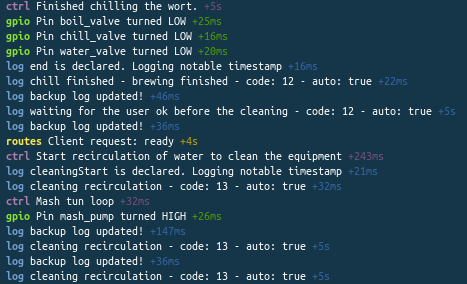
\includegraphics[height=5.0cm]{./Resources/simBrewing/simlog8.png}
		\caption{Recircula��o de �gua para limpeza preliminar}
		\label{console_sim_2:4}
	\end{subfigure}
	\captionsetup{justification=centering}
	\caption[Excertos relevantes das mensagens de depura��o do processo de simula��o da brassagem (parte 2)]{Excertos relevantes das mensagens de depura��o do processo de simula��o da brassagem (parte 2)}
	\label{console_sim_2}
\end{figure}

Em seguida, ap�s a certifica��o de que o processo de automa��o estava coerente com o processo de produ��o de cerveja e com as especifica��es do equipamento, por meio de ajustes incrementais nos c�digos-fonte do projeto, foram ligados � BBB: interfaces de pot�ncia aos pinos de GPIO, com LEDs ligados �s suas sa�das para inspe��o visual; rel�s de estado s�lido ligados diretamente aos pinos de GPIO da BBB respectivos ao controle dos resistores de pot�ncia --- � sa�da destes nada foi adicionado, uma vez que possuem LED indicador do estado da sa�da; e interface de pot�ncia ligada ao PWM, com o servo-motor acoplado � sua sa�da. O resultado desta simula��o � apresentado na figura \ref{proto_sim_1}, na qual o esfor�o de equiparar as fases documentadas com as das figuras \ref{console_sim_1} e \ref{console_sim_2} foi parcialmente efetivo: em fun��o do fato de que algumas partes de transi��o s�o r�pidas, n�o foi pr�tico documentar o equivalente ao \textit{log} do terminal em imagens est�ticas.

\begin{figure}[H]
	\centering
	\begin{subfigure}{.46\textwidth}
		\centering
		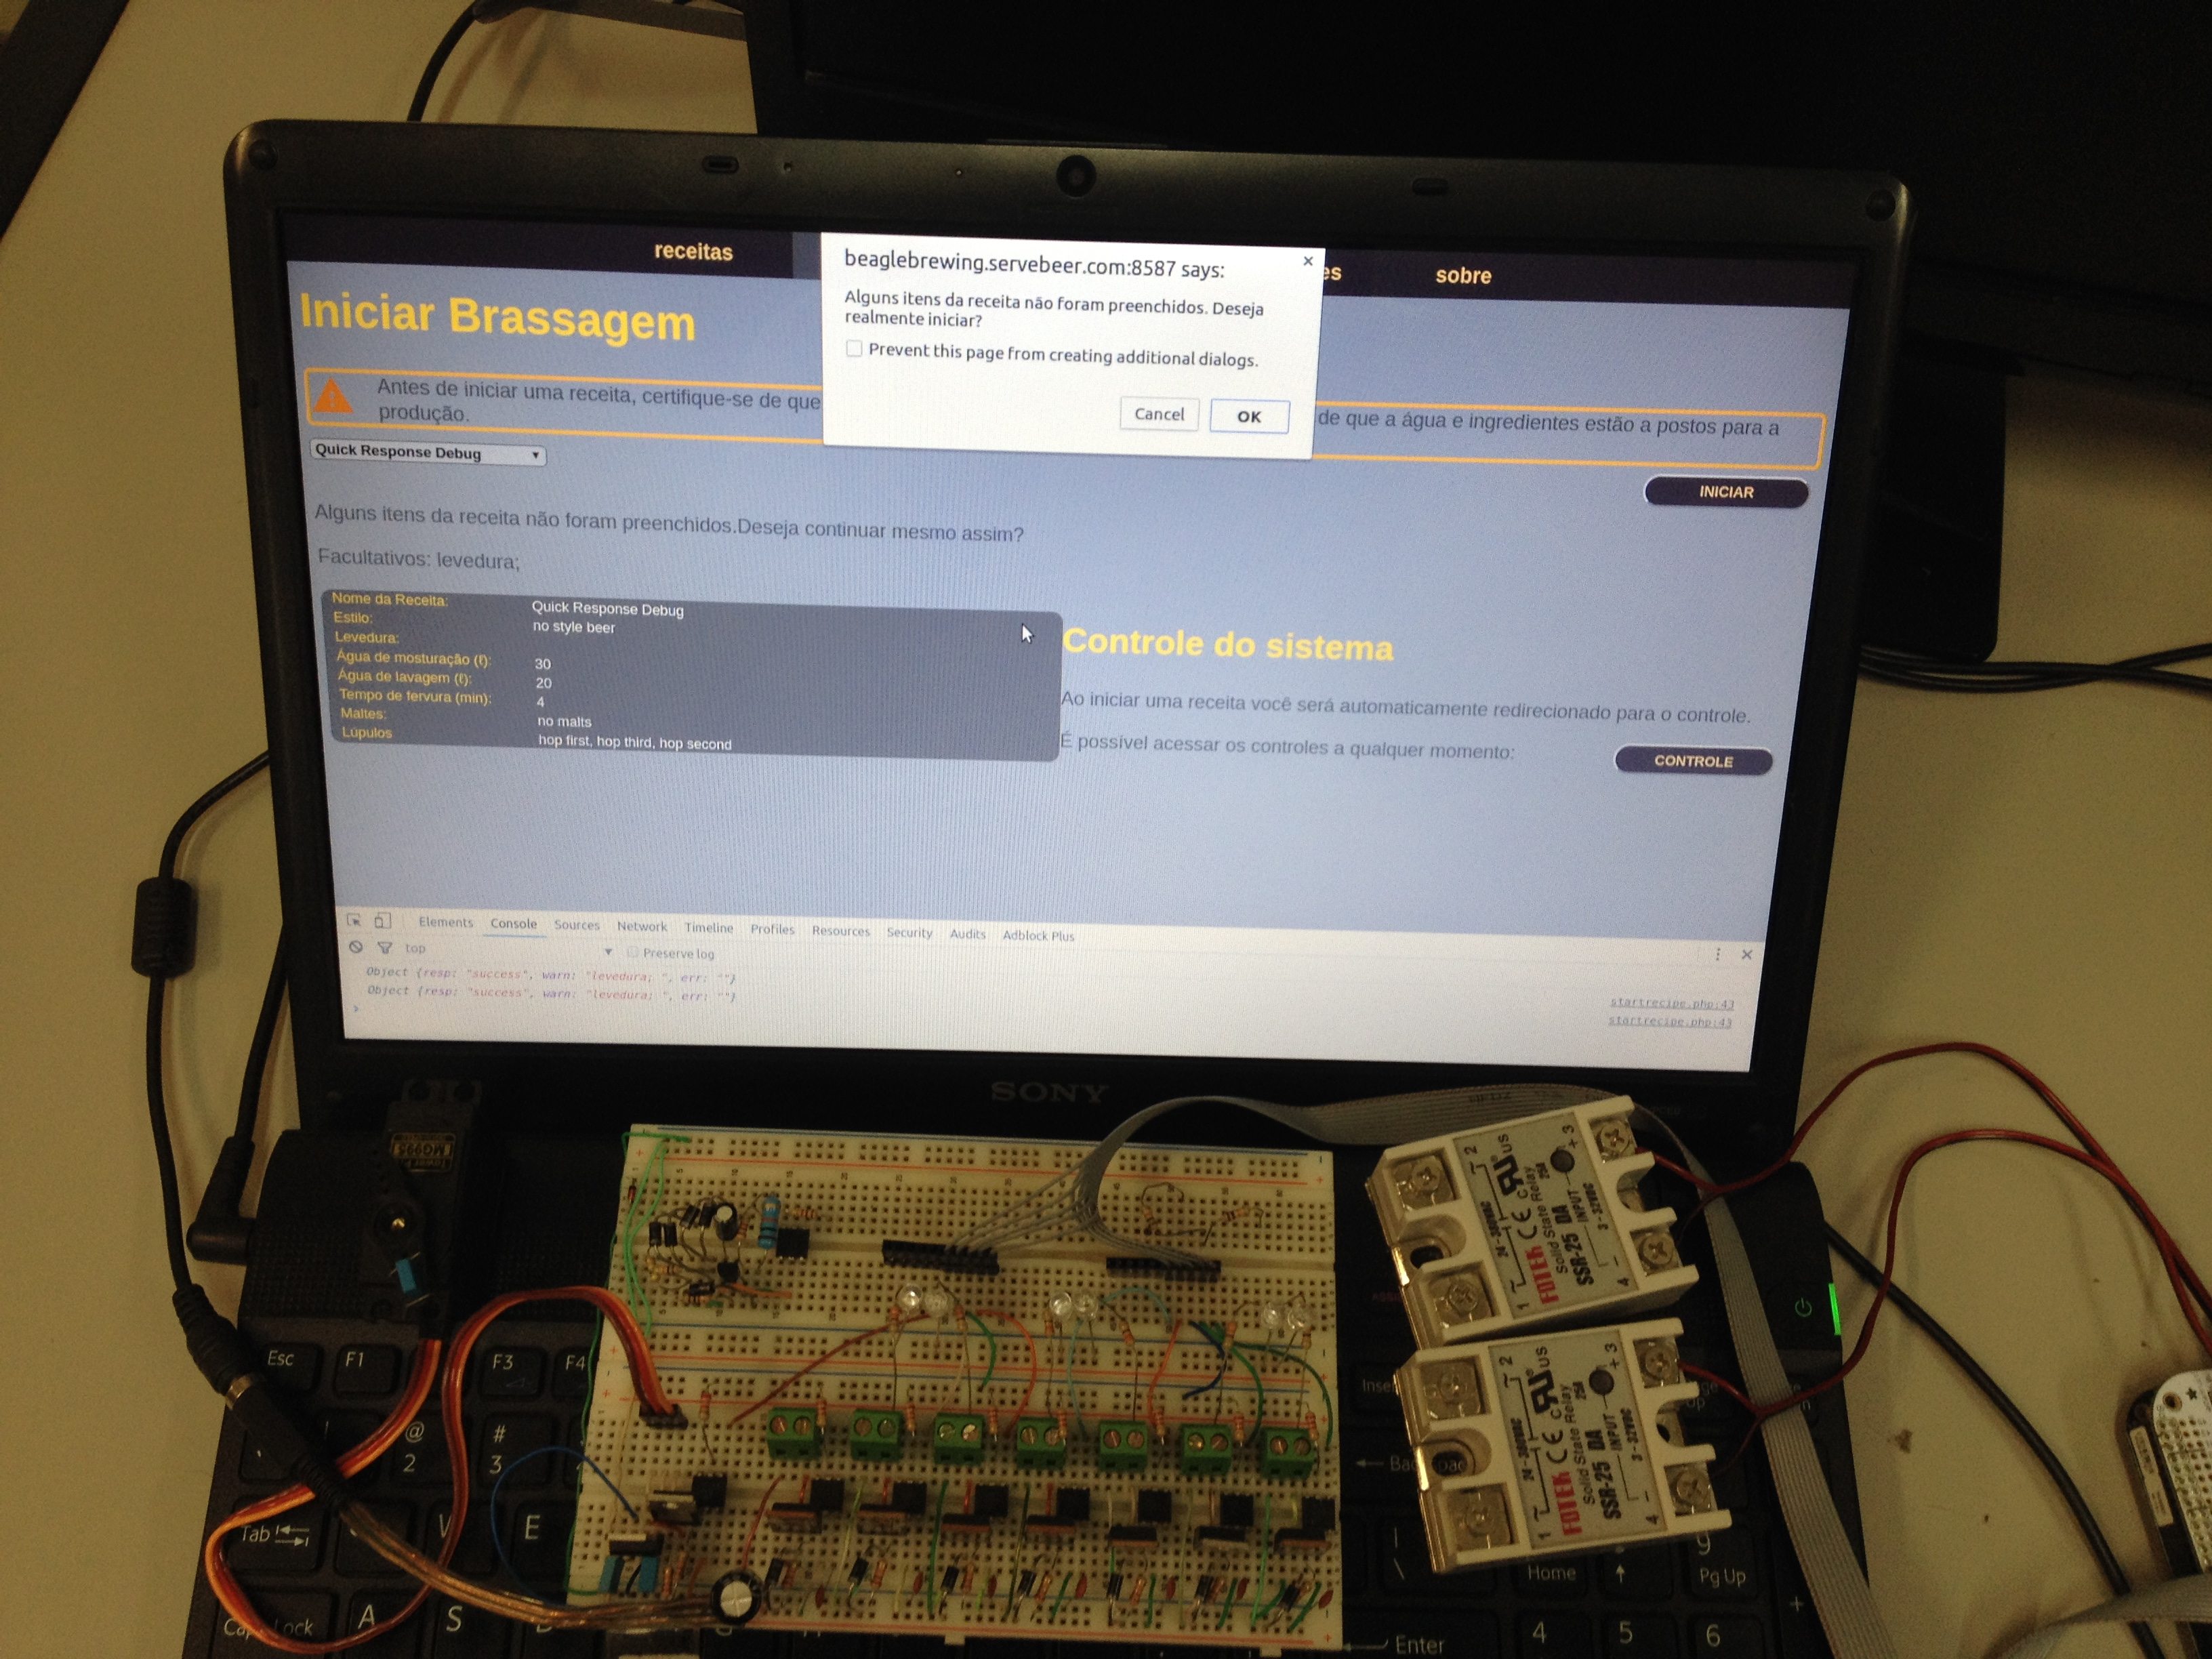
\includegraphics[height=5cm]{./Resources/simBrewing/sim_proto1.jpg}
		\caption{Acesso � GUI e in�cio da brassagem}
		\label{proto_sim_1:1}
	\end{subfigure}
	\begin{subfigure}{.46\textwidth}
		\centering
		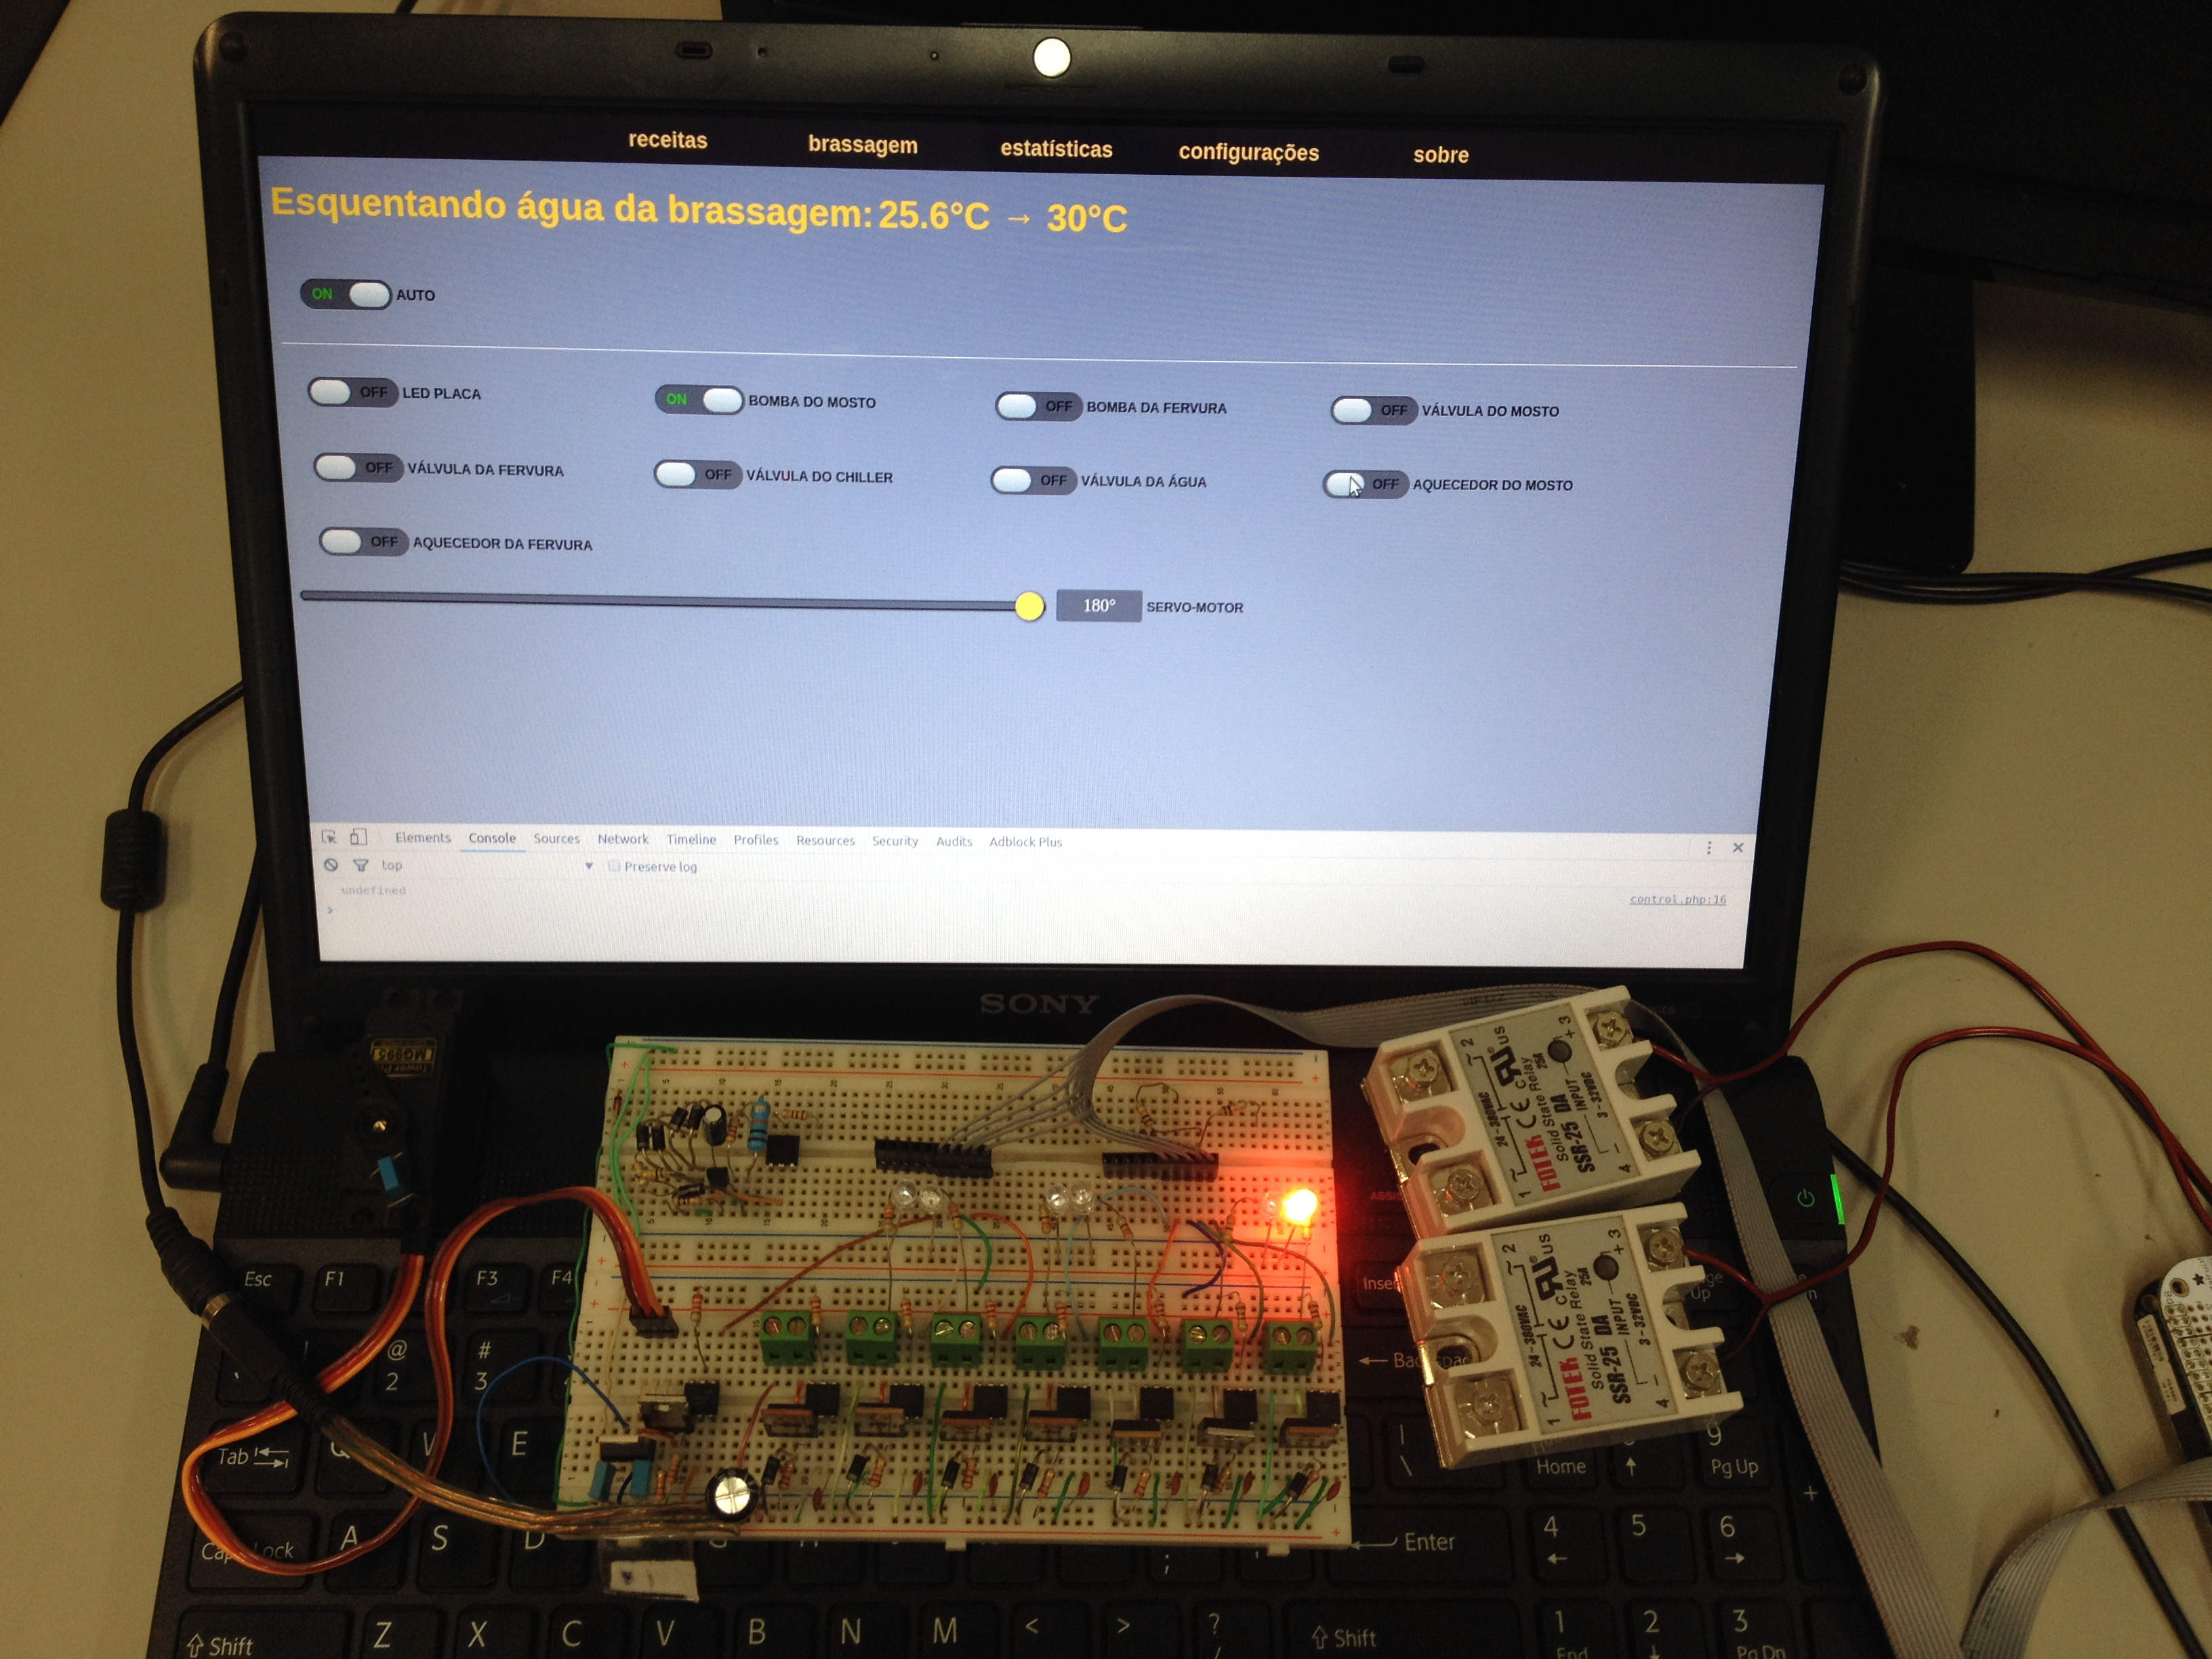
\includegraphics[height=5cm]{./Resources/simBrewing/sim_proto2.jpg}
		\caption{In�cio do controle de temperatura}
		\label{proto_sim_1:2}
	\end{subfigure}
	\begin{subfigure}{.46\textwidth}
		\centering
		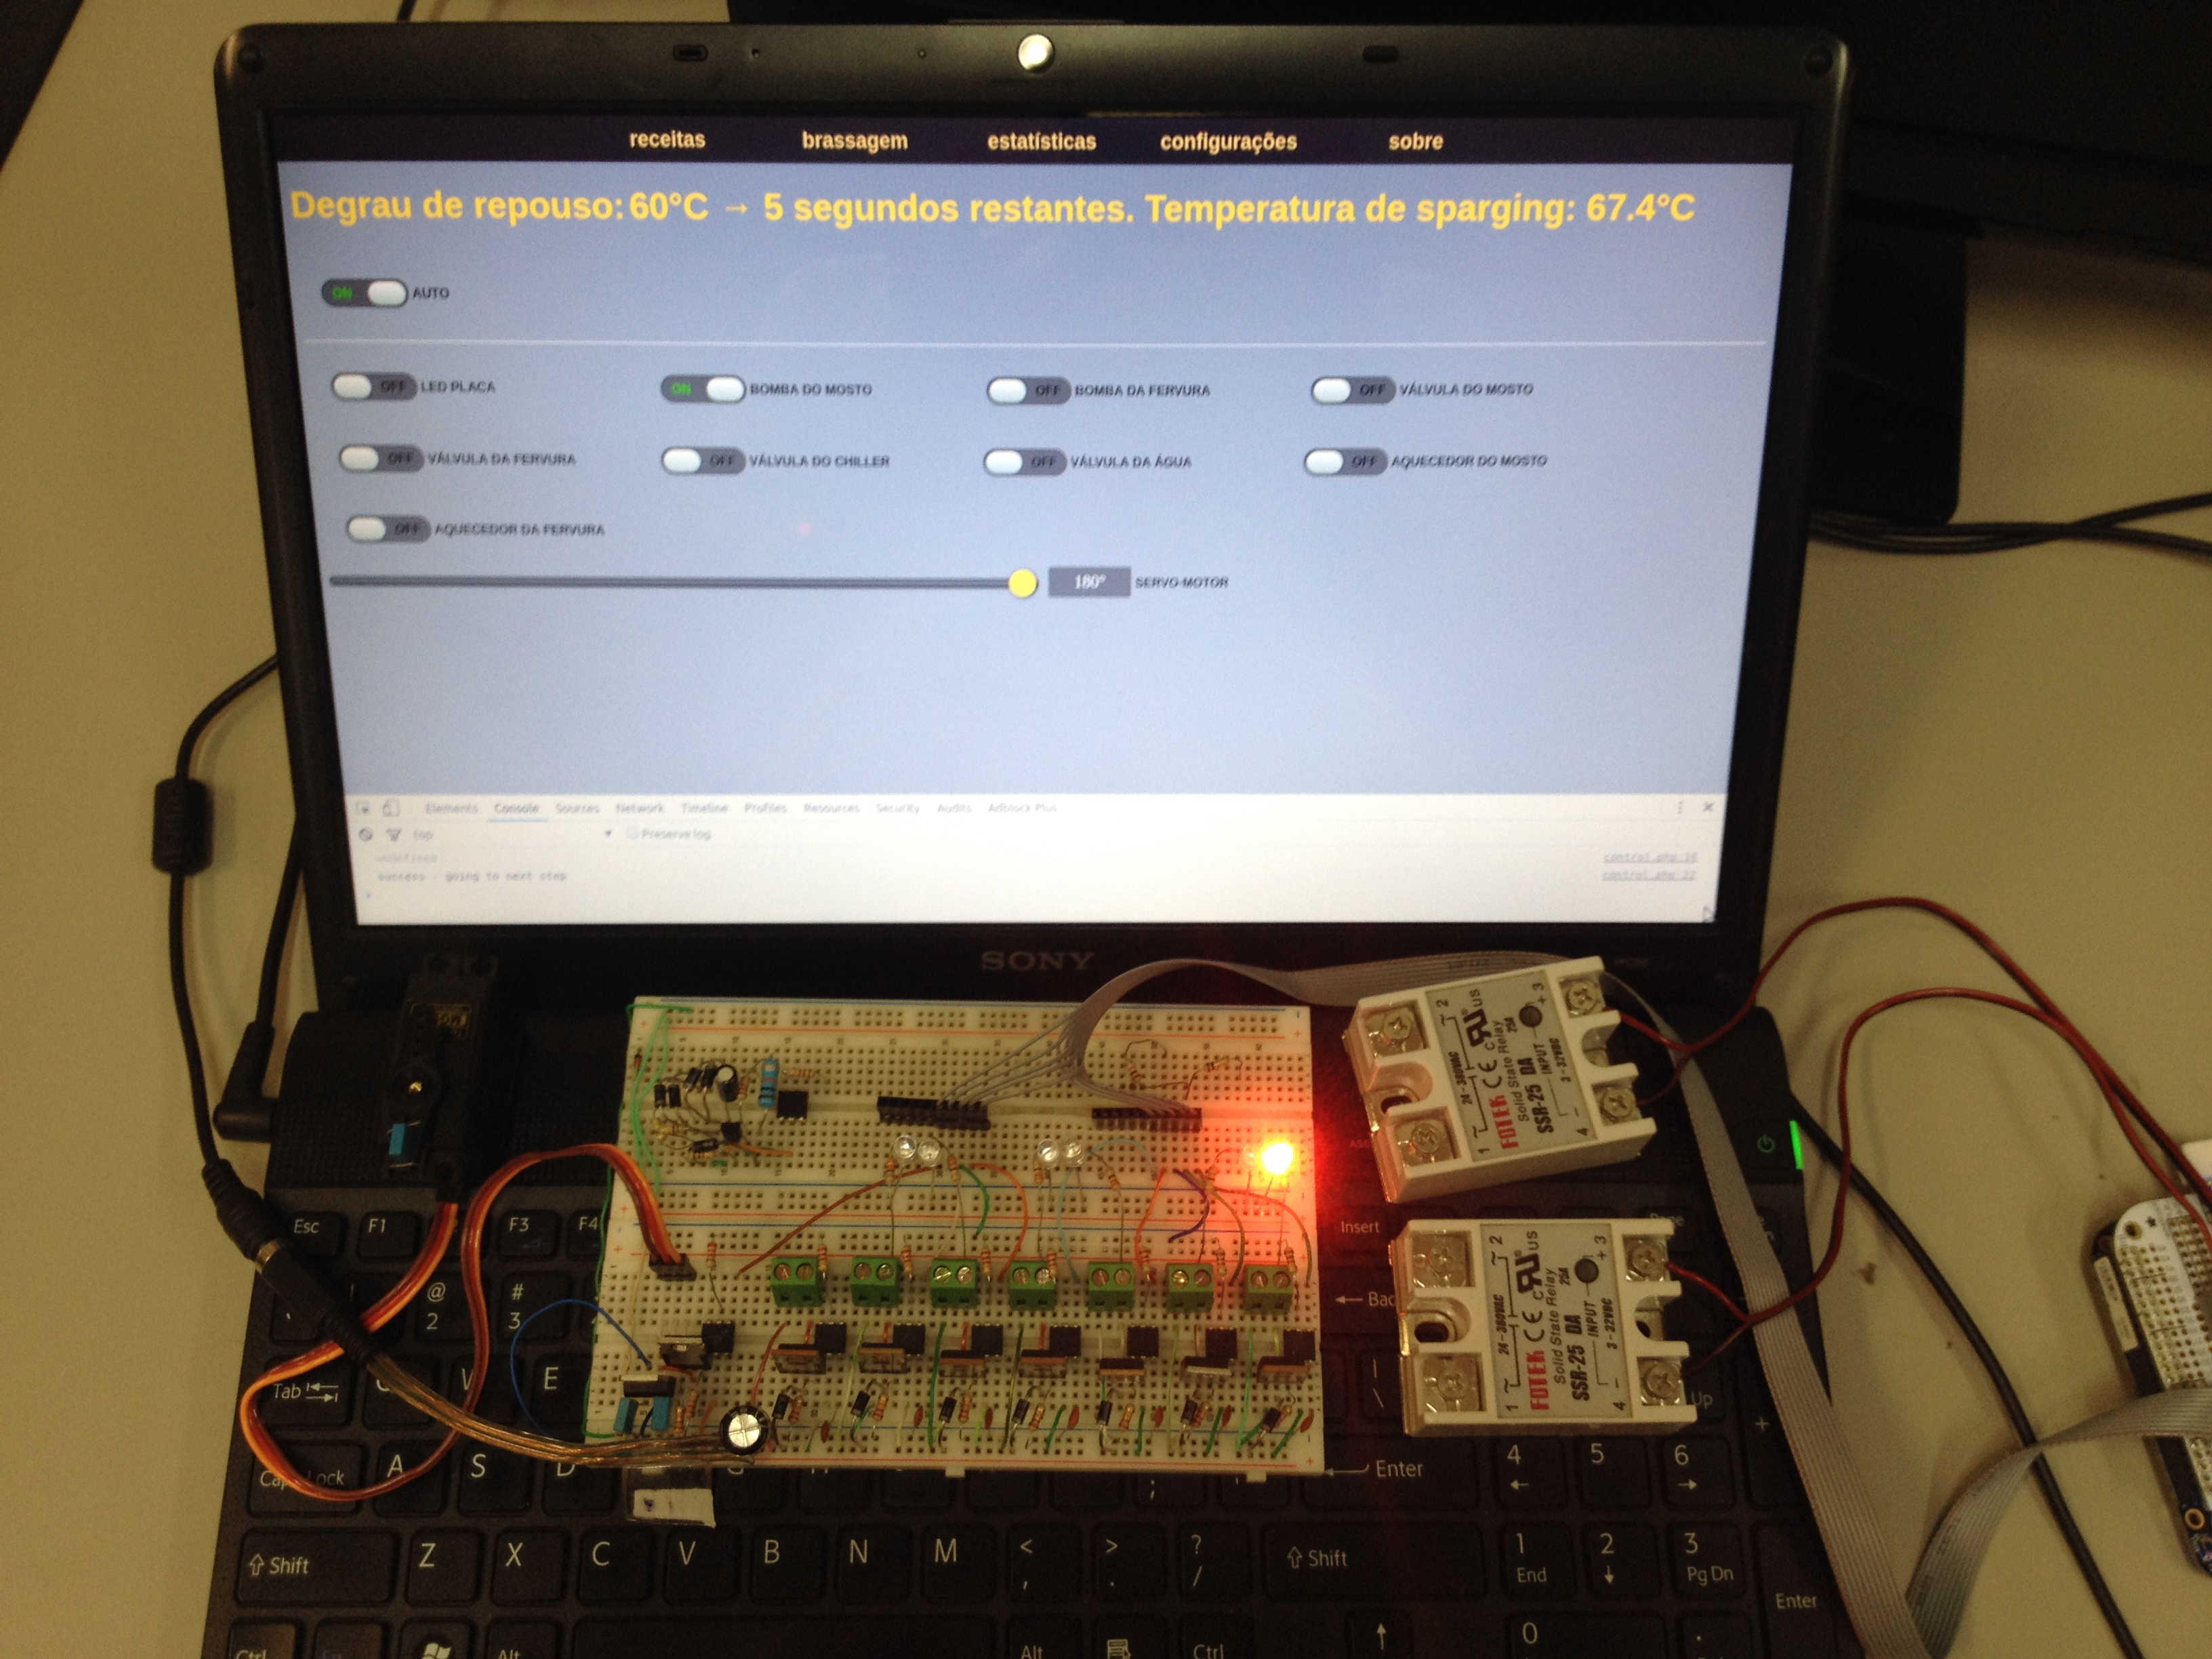
\includegraphics[height=5cm]{./Resources/simBrewing/sim_proto3.jpg}
		\caption{Final do controle de temperatura}
		\label{proto_sim_1:3}
	\end{subfigure}
	\begin{subfigure}{.46\textwidth}
		\centering
		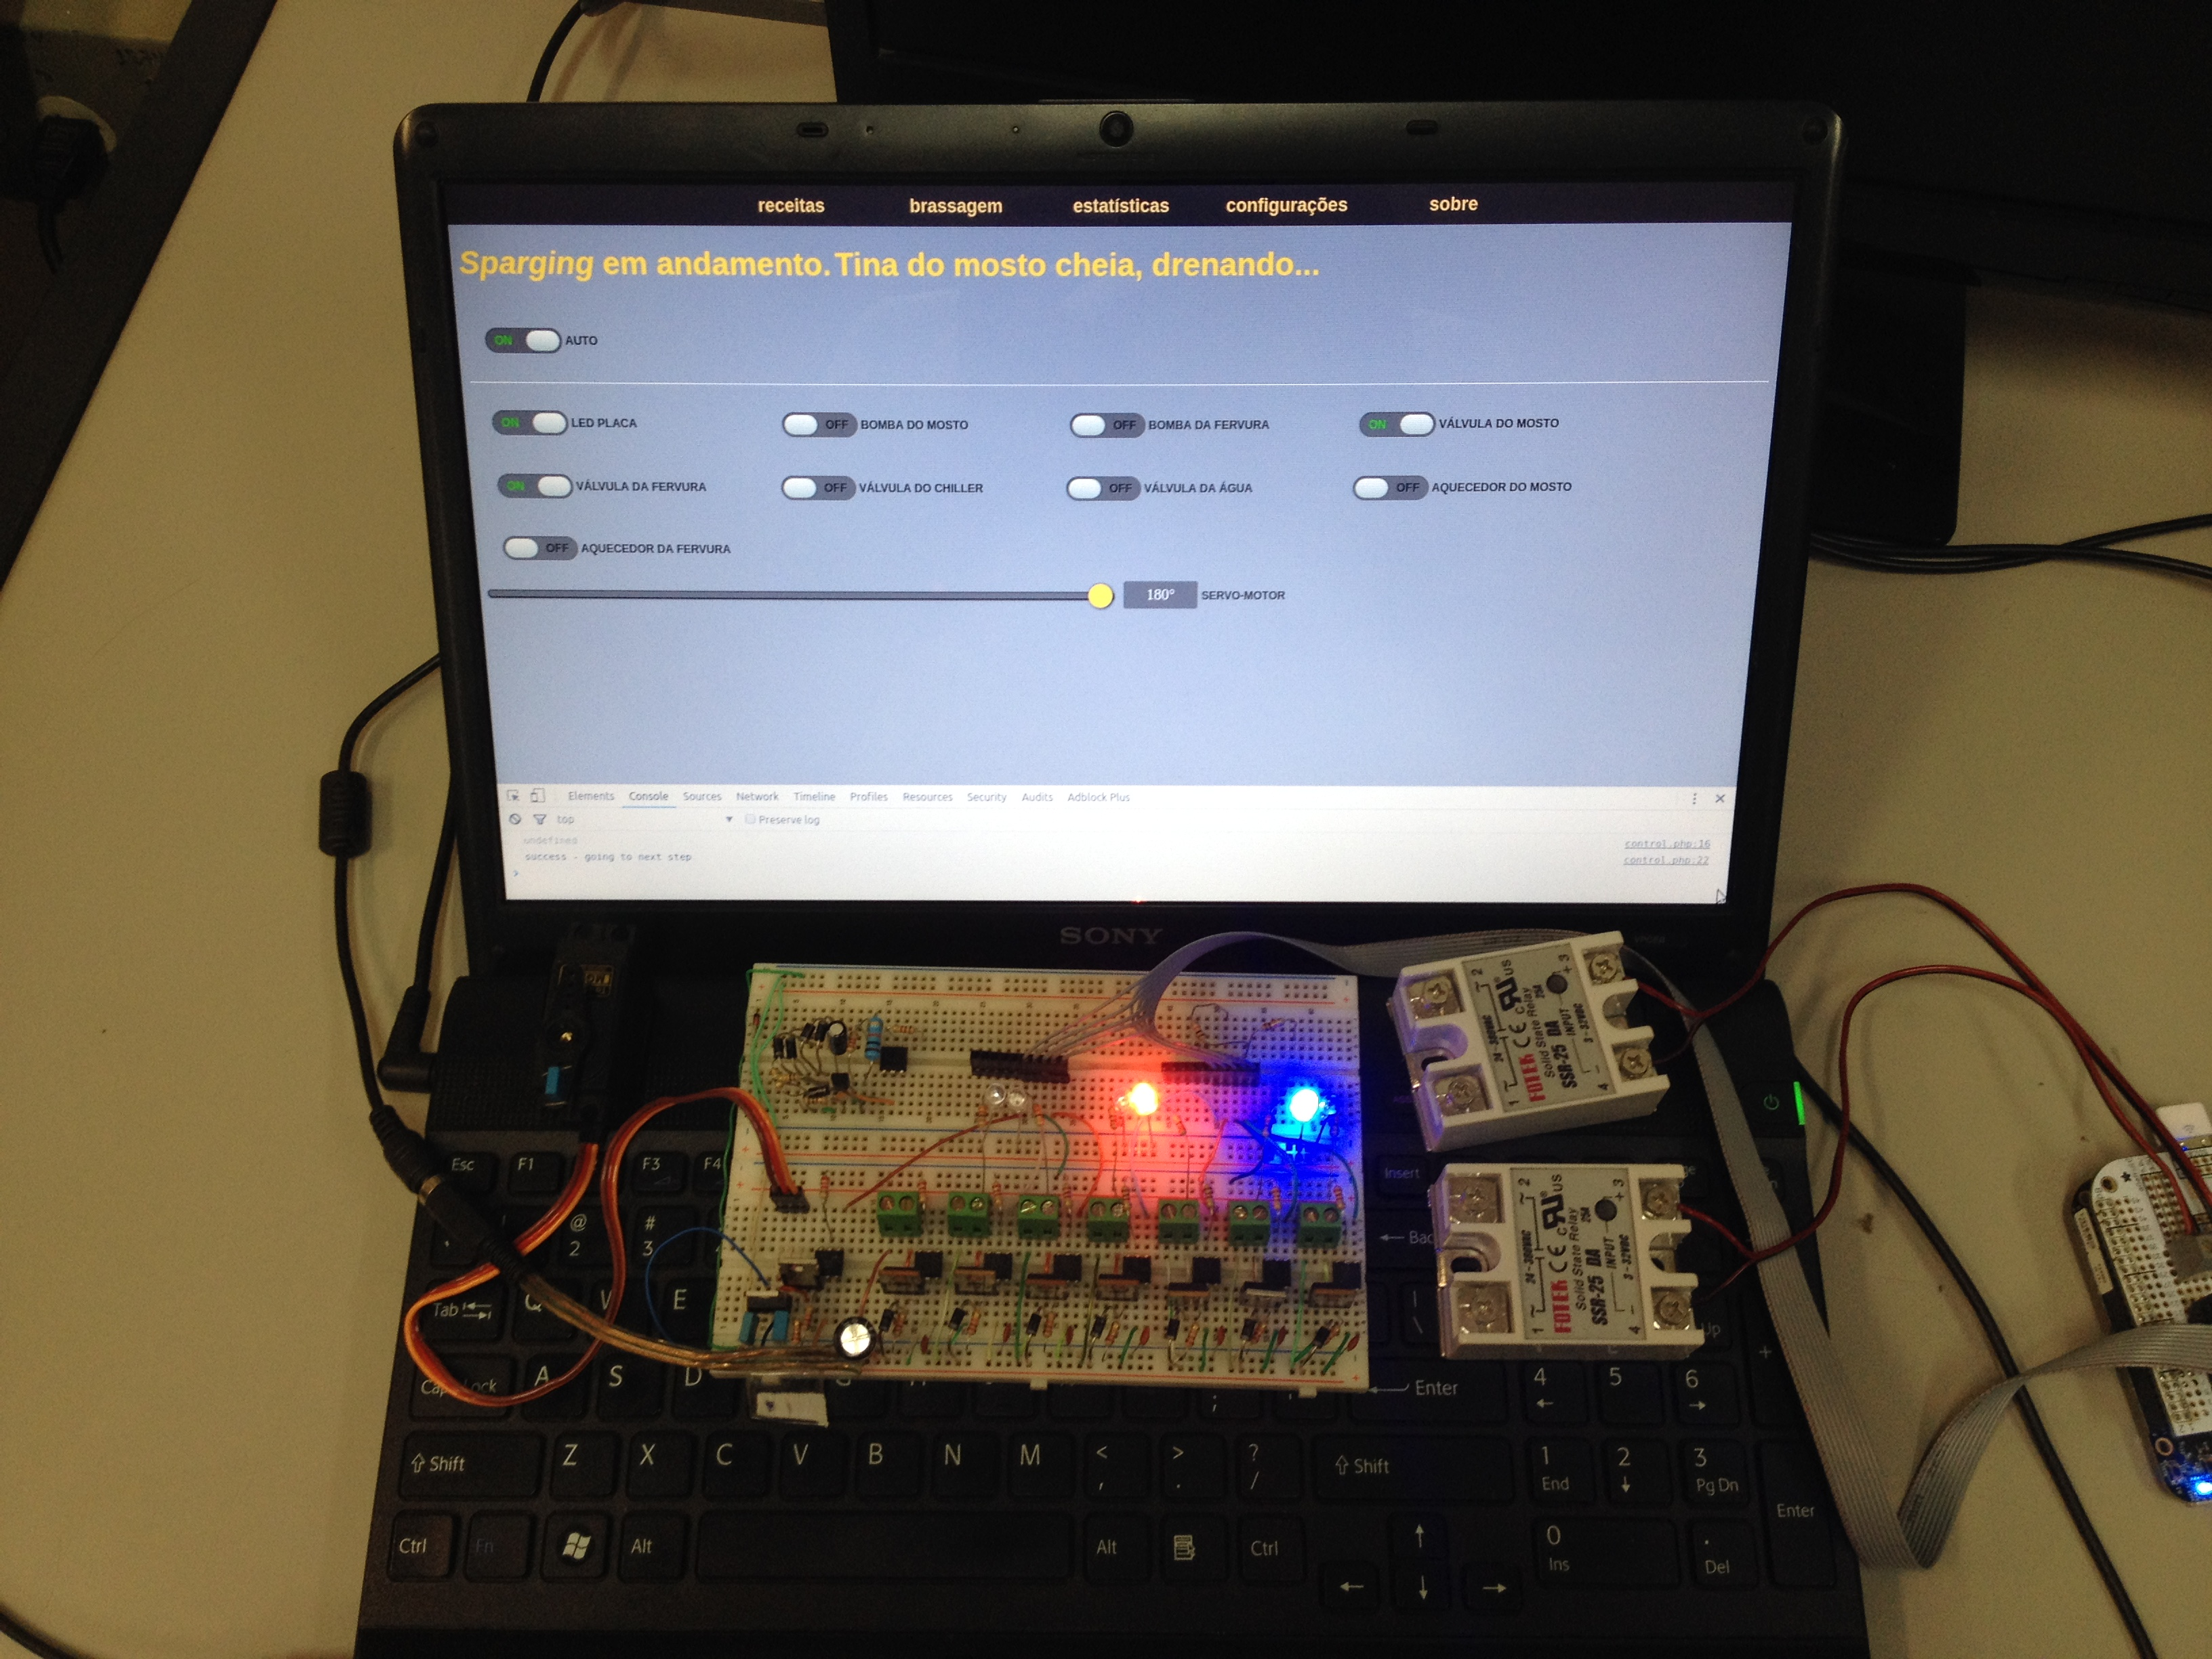
\includegraphics[height=5cm]{./Resources/simBrewing/sim_proto4.jpg}
		\caption{In�cio da lavagem dos gr�os (\textit{sparging})}
		\label{proto_sim_1:4}
	\end{subfigure}
	\begin{subfigure}{.46\textwidth}
		\centering
		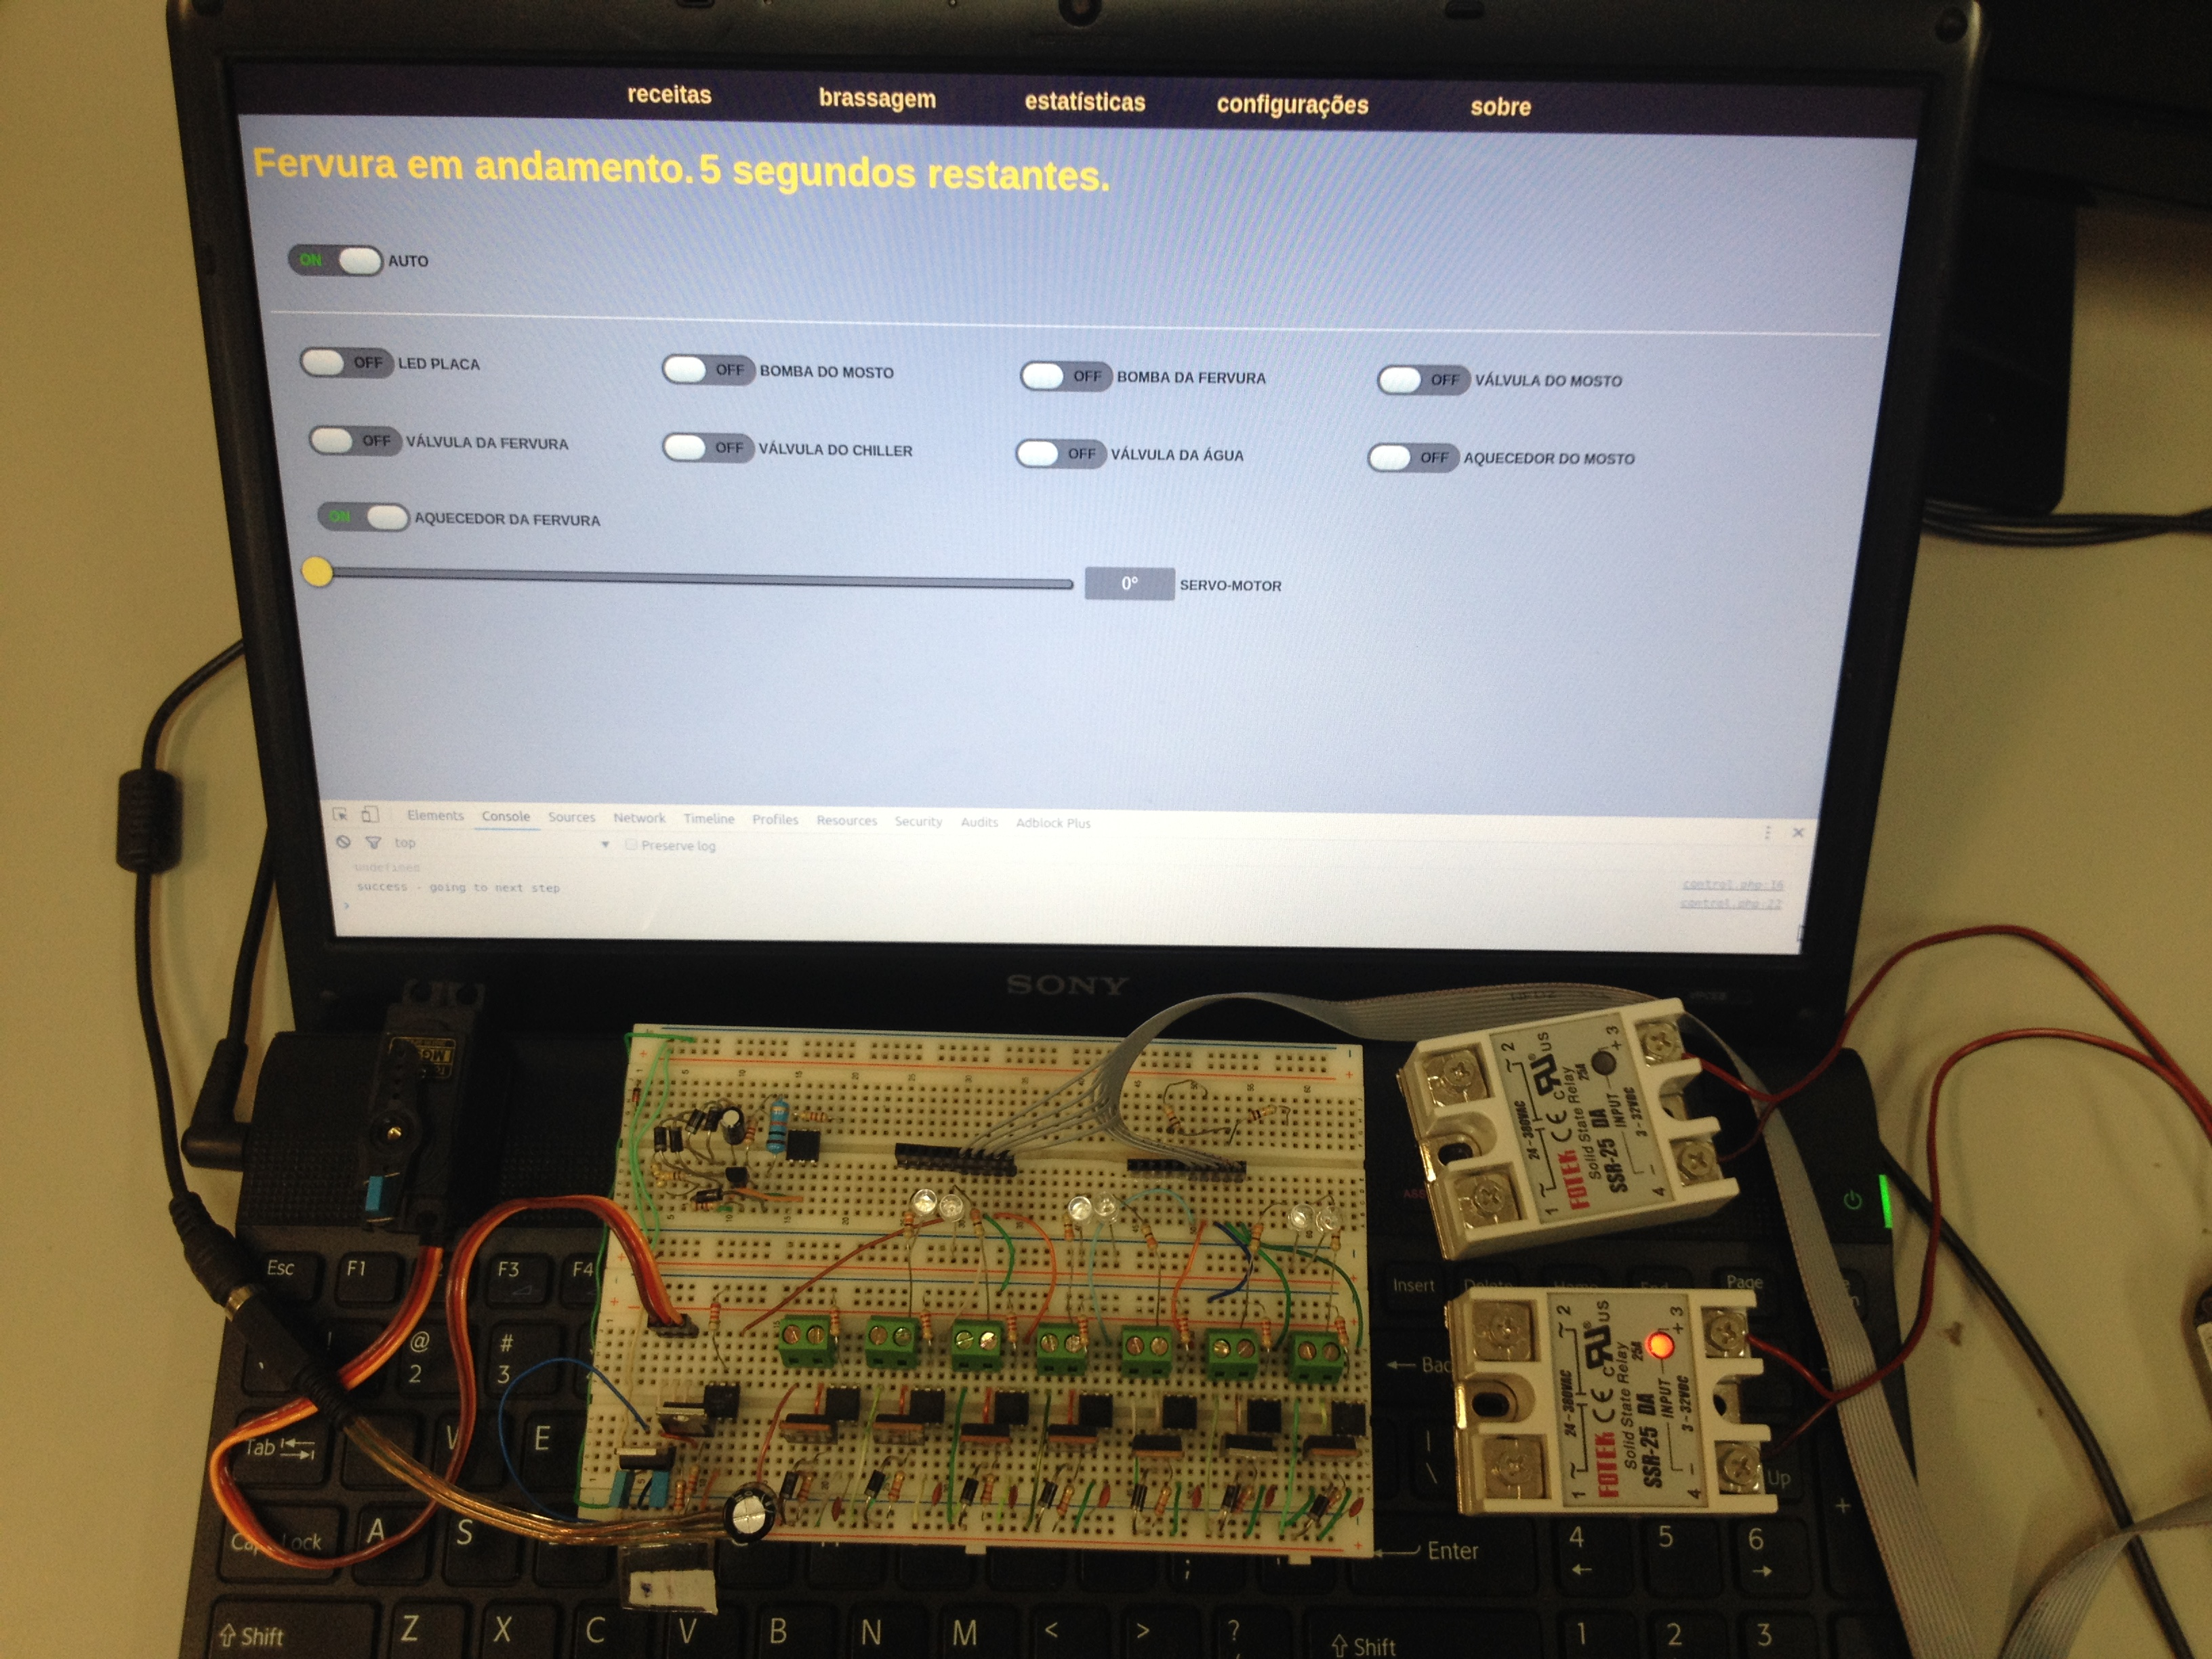
\includegraphics[height=5cm]{./Resources/simBrewing/sim_proto5.jpg}
		\caption{In�cio da fervura do mosto}
		\label{proto_sim_1:5}
	\end{subfigure}
	\begin{subfigure}{.46\textwidth}
		\centering
		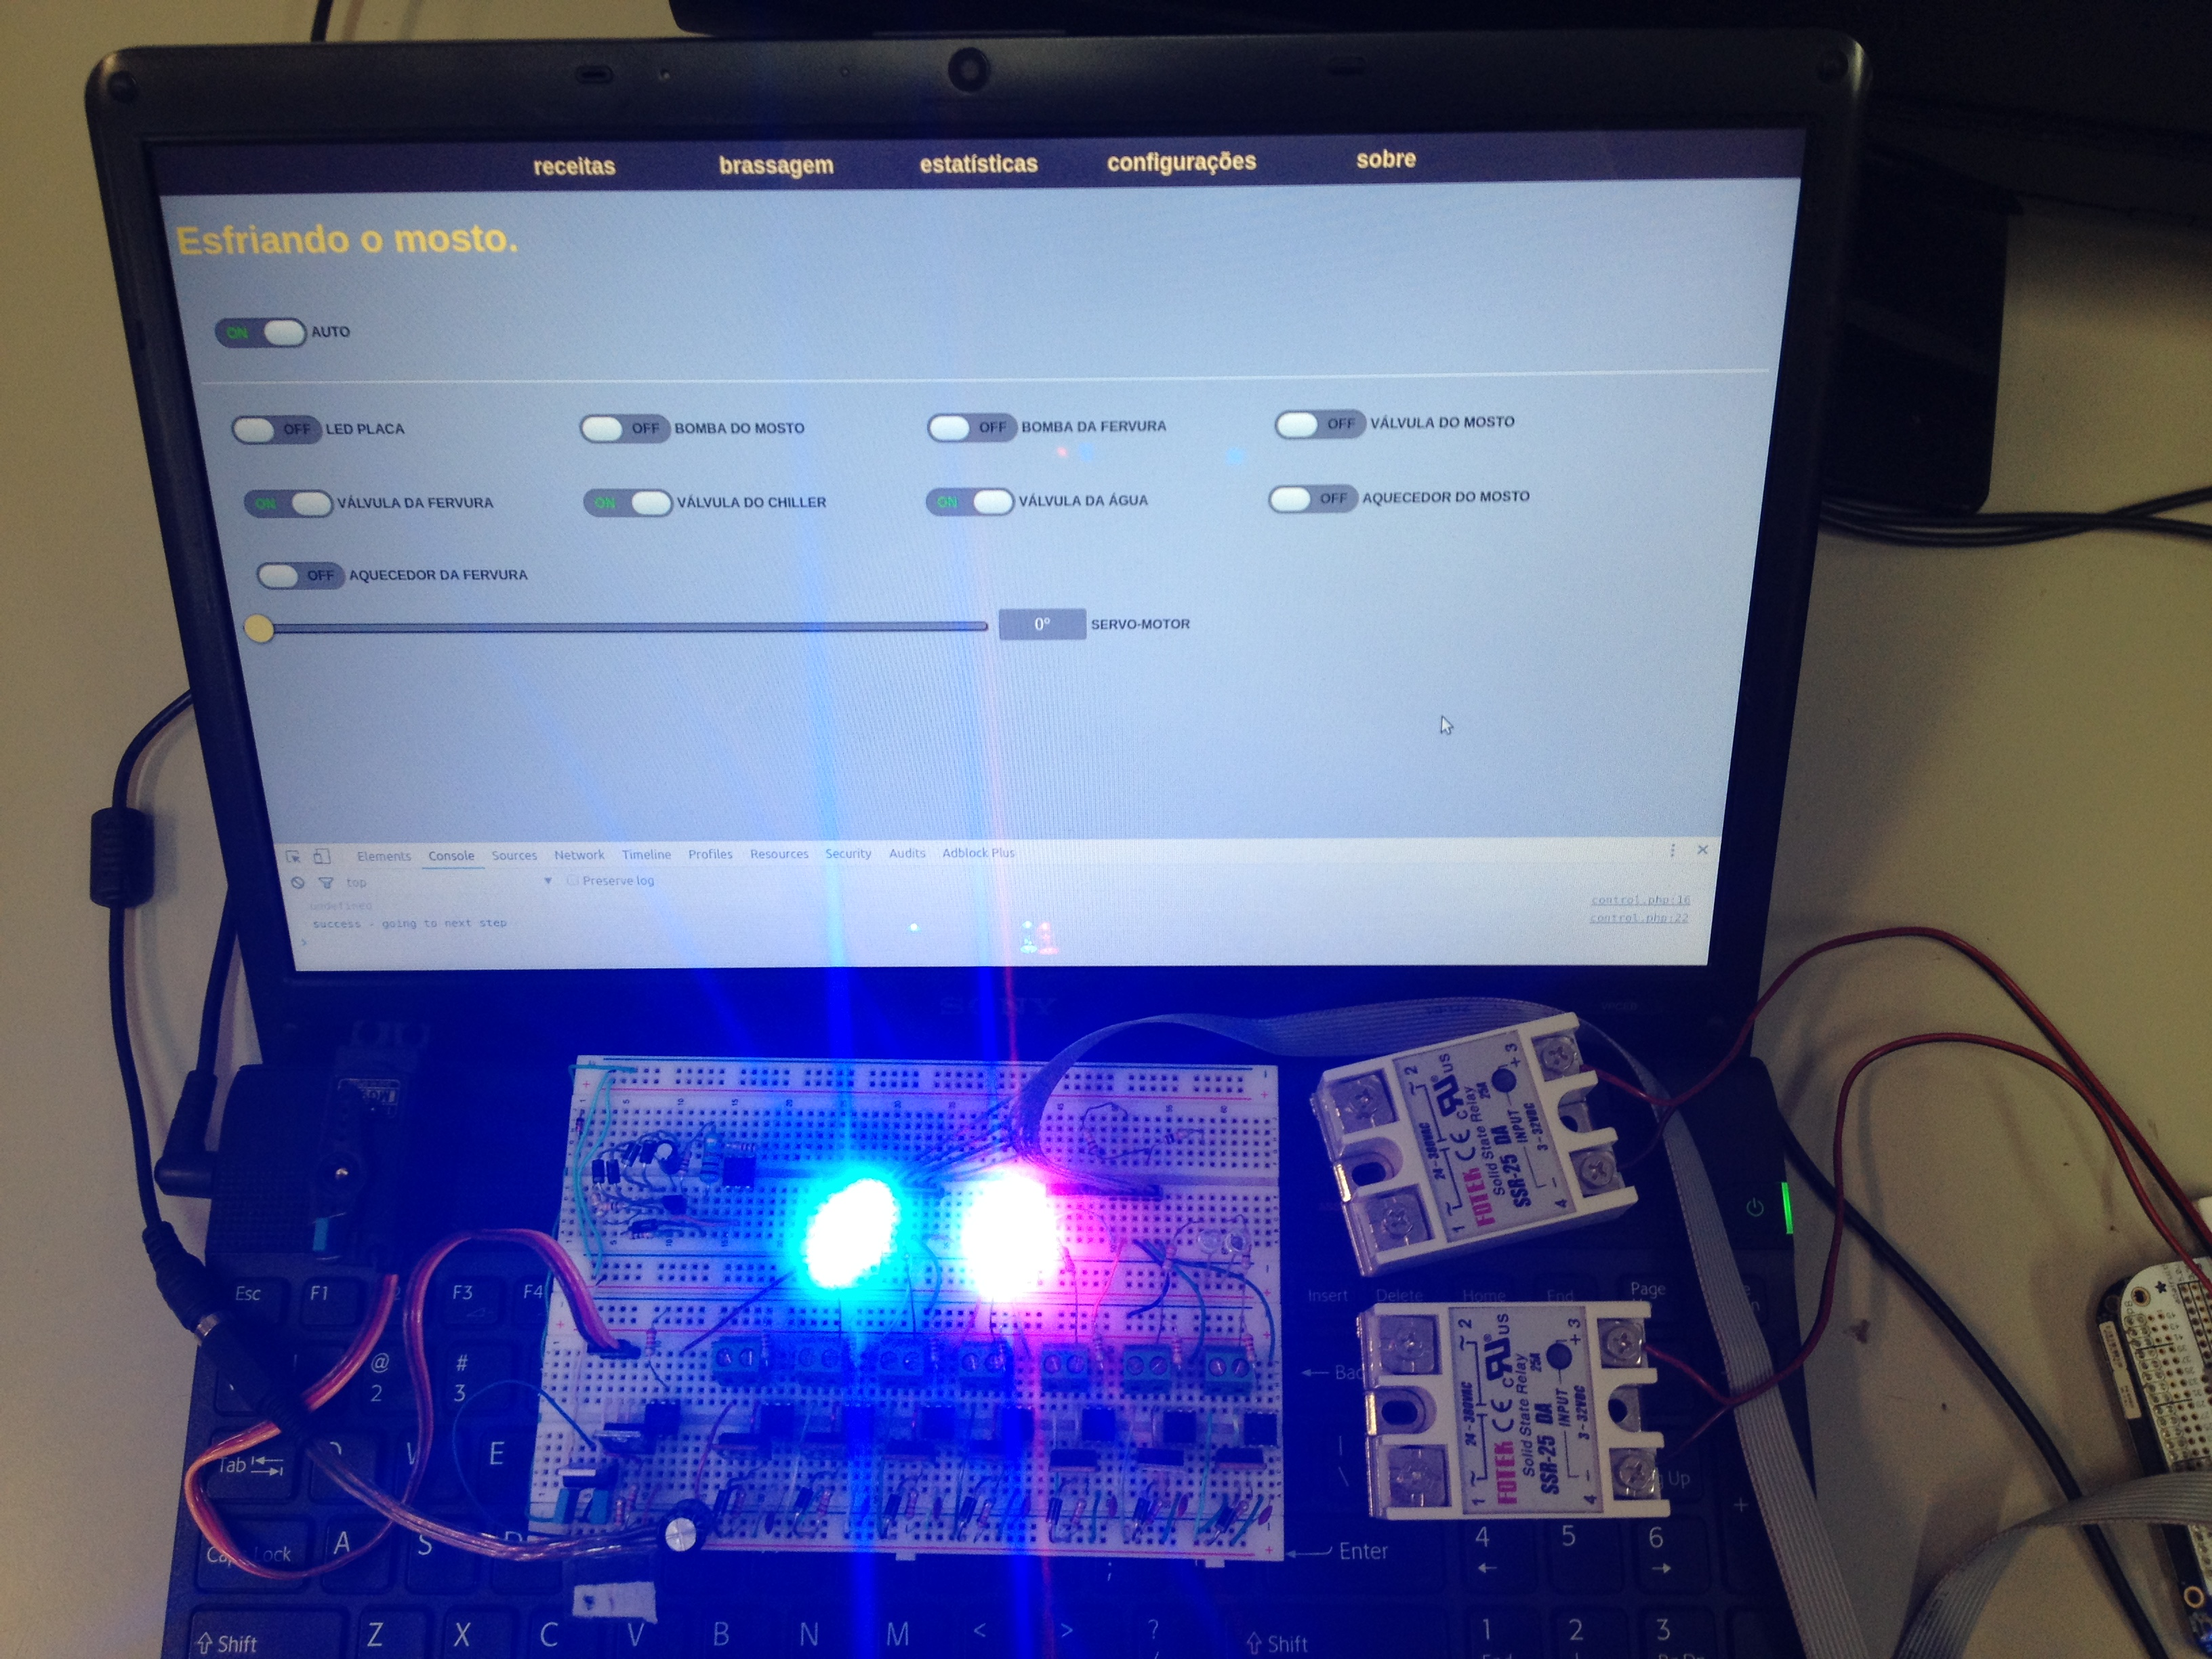
\includegraphics[height=5cm]{./Resources/simBrewing/sim_proto6.jpg}
		\caption{In�cio do resfriamento do mosto}
		\label{proto_sim_1:6}
	\end{subfigure}
	\begin{subfigure}{.46\textwidth}
		\centering
		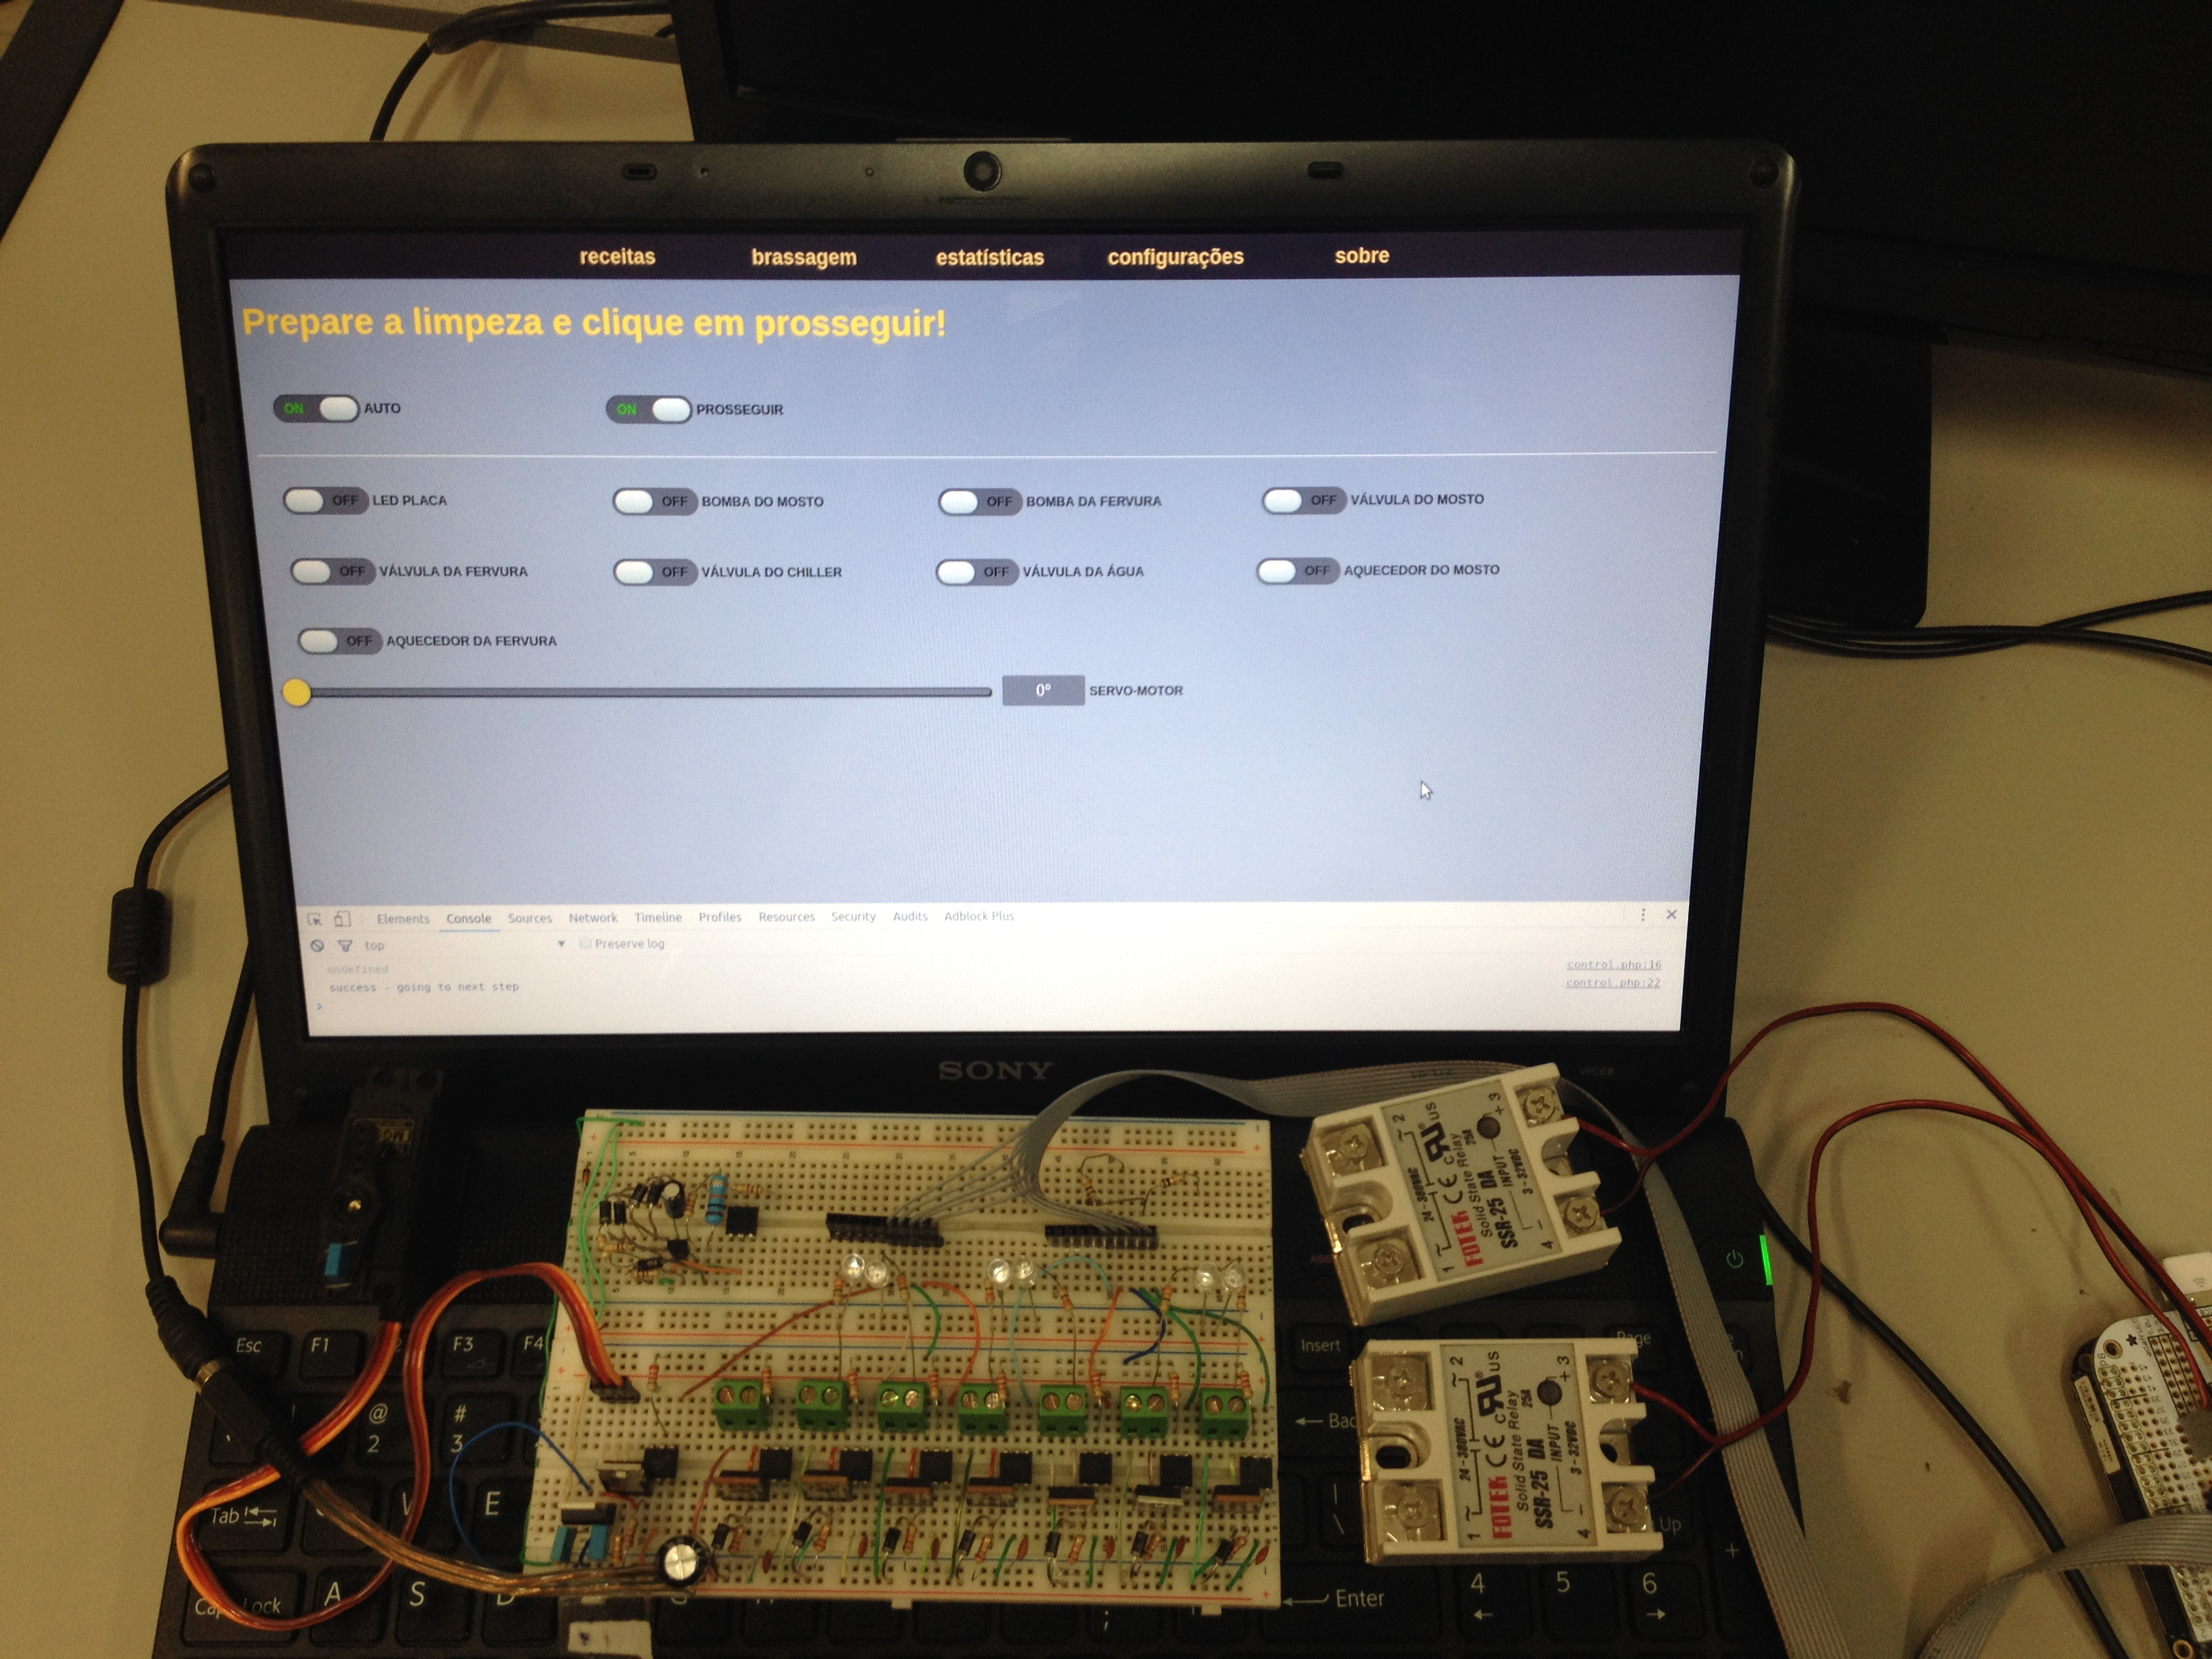
\includegraphics[height=5cm]{./Resources/simBrewing/sim_proto7.jpg}
		\caption{Recircula��o de �gua para limpeza preliminar}
		\label{proto_sim_1:7}
	\end{subfigure}
	\captionsetup{justification=centering}
	\caption[Momentos relevantes da simula��o observados na GUI e nos circuitos de interface de pot�ncia]{Momentos relevantes da simula��o observados na GUI e nos circuitos de interface de pot�ncia}
	\label{proto_sim_1}
\end{figure}  

Quanto aos recursos de hardware consumidos durante o processo de brassagem, foi gravado um v�deo da tela do computador usando o software de captura de tela \textit{SimpleScreenRecorder} e, posteriormente, o consumo de mem�ria e CPU do sistema foi sintetizado na tabela \ref{sim_res_cpu}. � importante notar que o uso de recursos do comando \textit{htop}, usado como monitor de recursos para este caso, � da ordem de 10\% e portanto n�o � desprez�vel, e tamb�m os dados da tabela \ref{sim_res_cpu} s�o valores instant�neos e n�o representam nenhum tipo de infer�ncia estat�stica.

Tamb�m foi usado o comando \textit{sar} do pacote \textit{sysstat} para gerar um arquivo de \textit{log} de performance da CPU, mem�ria RAM e volume de tr�fego de rede IPv4, a partir do qual foram gerados os gr�ficos apresentados nas figuras \ref{sar_performance} e \ref{sar_network}, que apresentam o uso de CPU e mem�ria RAM; e recursos de rede utilizados em fun��o do tempo, respectivamente.

\begin{table}[H]
	\centering
	\captionsetup{justification=centering}
	\caption[Consumo de recursos de mem�ria e processamento da BBB ao longo do processo de brassagem]{Consumo de recursos de mem�ria e processamento da BBB ao longo do processo de brassagem}
	\label{sim_res_cpu}
	\begin{tabular}{ | M{7.5cm} | M{3cm} | M{3cm} |}
		\hline
		\textbf{Fase da brassagem} & \textbf{Mem�ria RAM (Mb)} & \textbf{Consumo da CPU (\%)}\\ \hline
		Sele��o da receita & 138 & 10 \\ \hline
		Autoriza��o do in�cio de produ��o & 138 & 22 \\ \hline
		Aquecimento da �gua da brassagem & 140 & 28 \\ \hline
		Transi��o de in�cio do controle de temperatura & 140 & 34 \\ \hline
		Controle de rampa & 140 & 20 \\ \hline
		Controle de degrau & 140 & 35 \\ \hline
		Fim do controle de temperatura & 141 & 28 \\ \hline
		Detec��o de transbordamento & 141 & 24 \\ \hline
		Lavagem dos gr�os & 141 & 29 \\ \hline
		Fim da lavagem & 142 & 34 \\ \hline
		Fervura & 143 & 31 \\ \hline
		Resfriamento do mosto & 139 & 14 \\ \hline
		Come�o da recircula��o de limpeza & 139 & 27 \\ \hline
		Fim do processo --- ocioso & 139 & 15 \\ \hline
	\end{tabular}
\end{table}

\begin{figure}[H]
	\centering
	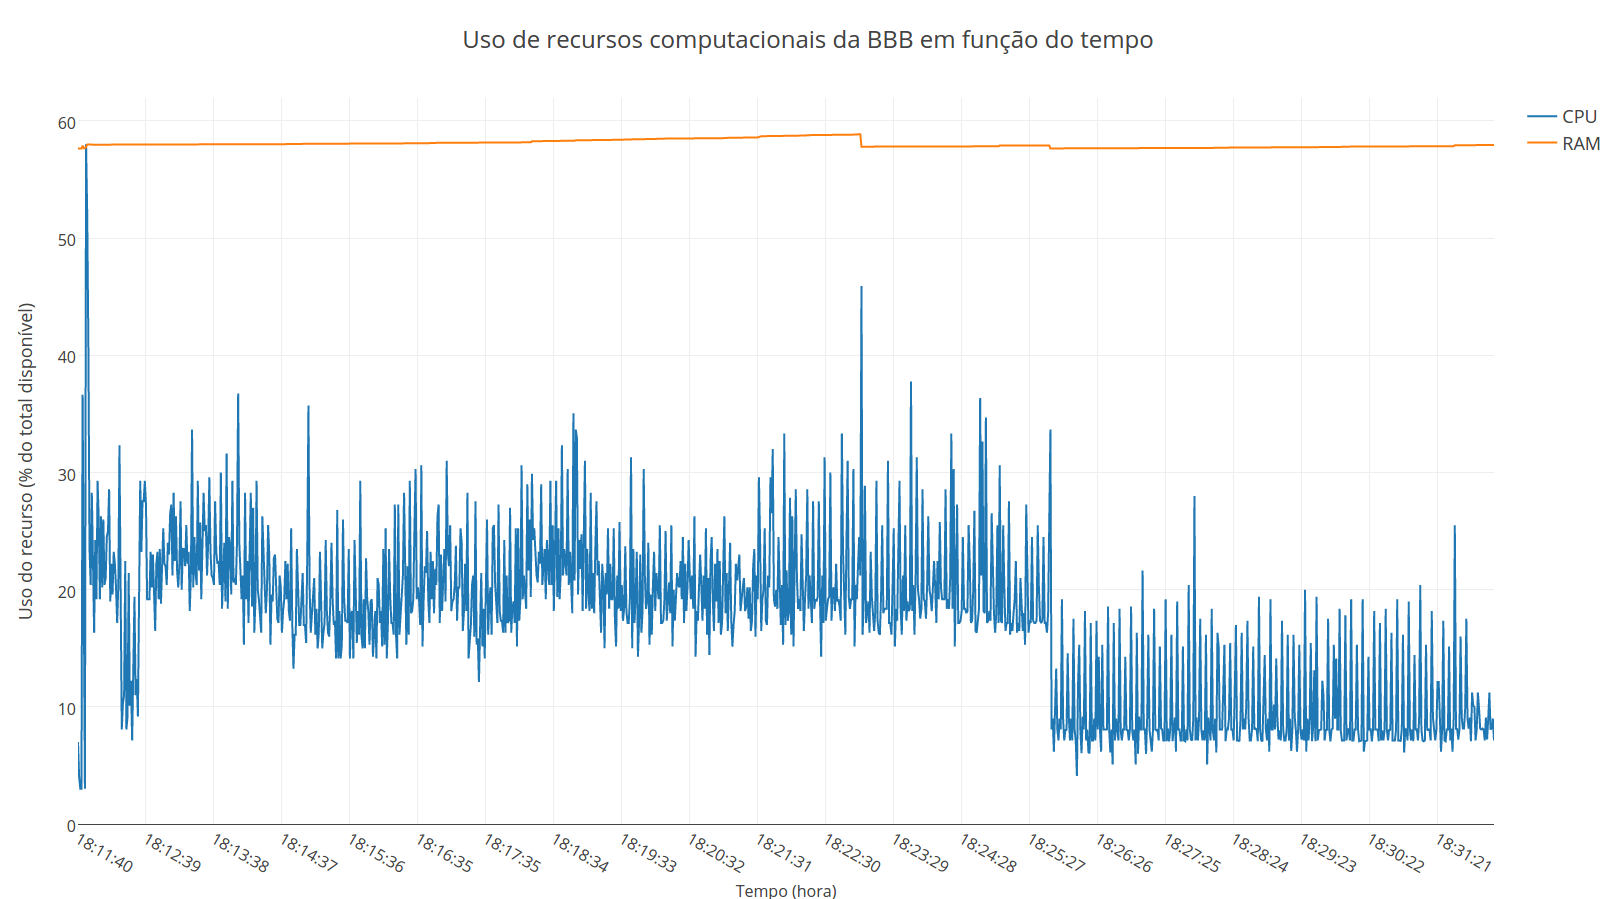
\includegraphics[scale=0.25]{./Resources/sar_cpu_ram_sim.png}
	\captionsetup{justification=centering}
	\caption[Gr�fico de consumo de recursos de CPU e mem�ria RAM da BBB em fun��o do tempo, durante uma simula��o de brassagem]{Gr�fico de consumo de recursos de CPU e mem�ria RAM da BBB em fun��o do tempo, durante uma simula��o de brassagem}
	\label{sar_performance}
\end{figure}

\begin{figure}[H]
	\centering
	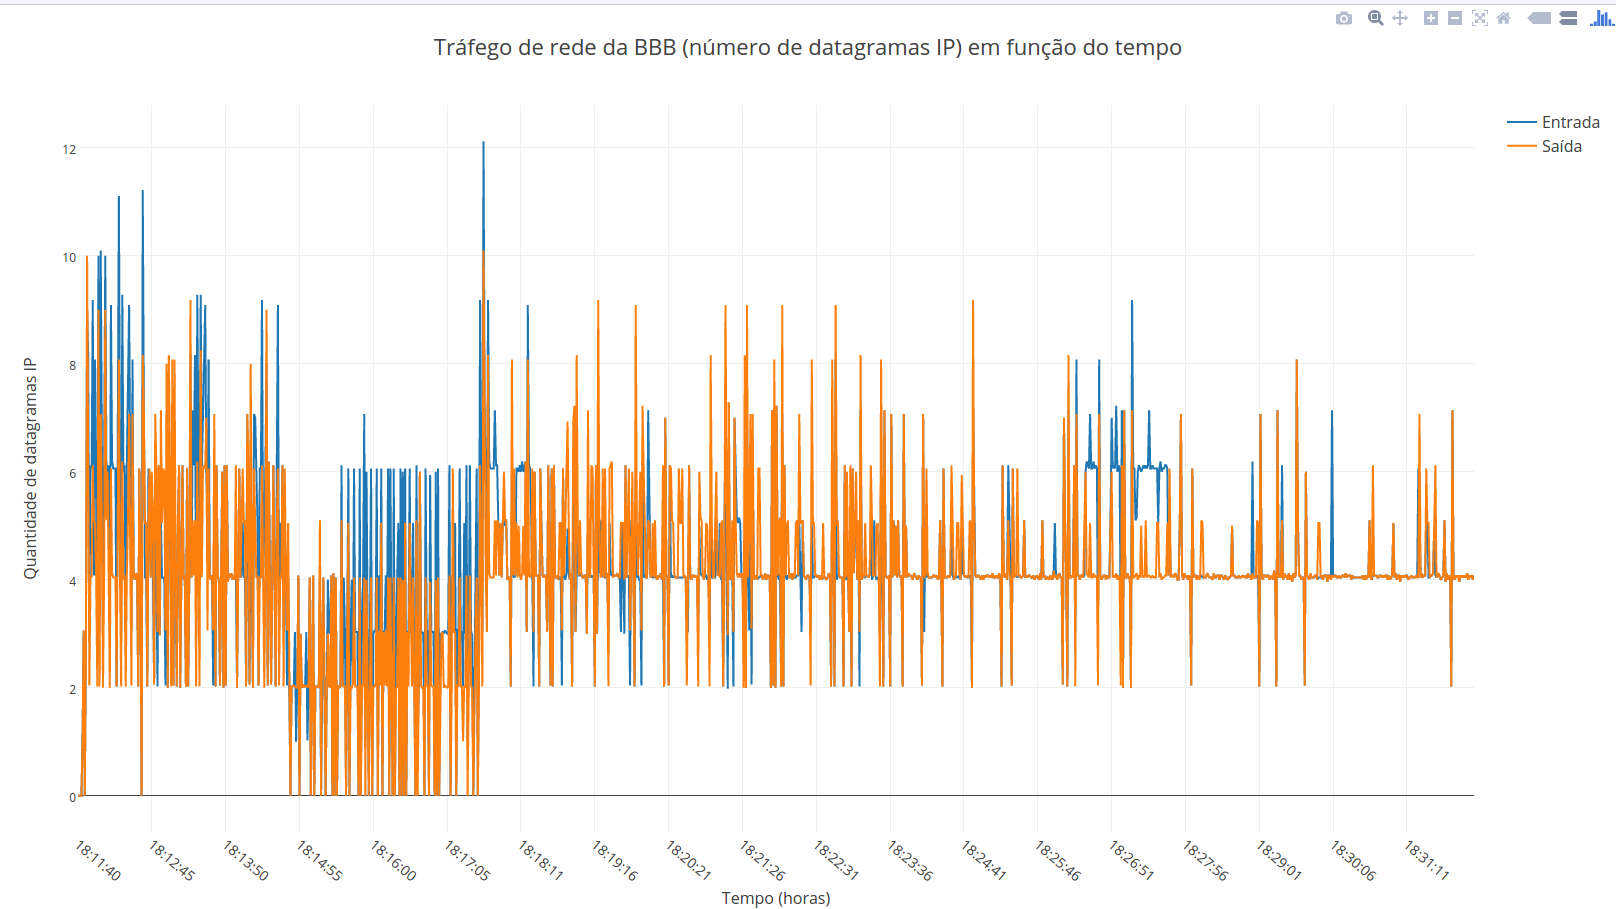
\includegraphics[scale=0.25]{./Resources/sar_net_sim.png}
	\captionsetup{justification=centering}
	\caption[Gr�fico de consumo de recursos de rede da BBB em fun��o do tempo, durante uma simula��o de brassagem]{Gr�fico de consumo de recursos de rede da BBB em fun��o do tempo, durante uma simula��o de brassagem}
	\label{sar_network}
\end{figure}

A partir dos dados obtidos, constatou-se que os recursos de processamento (CPU) ficaram abaixo de 40\%, salvo em um �nico ponto do gr�fico da figura \ref{sar_performance}, indicando que a BBB trabalhou muito abaixo do seu limite de processamento. Com rela��o � mem�ria RAM, foi observado que seu uso est� entre 55\% e 60\%. � not�vel a partir da observa��o do gr�fico que, ap�s o fim do processo de fervura, a quantidade de processamento demandada pela BBB foi reduzida pela metade.






%%%%%%%%%%%%%%%%%%%%%%%%%%%%%%%%%%%%%%%%%%%%%%%%%%%%%%%%%%%%%%%%%%%%%%%%%%

\section{Interface de usu�rio}
\label{resIntUser}

Nesta se��o s�o apresentados os resultados do desenvolvimento da interface de usu�rio. 

A p�gina inicial � composta de uma imagem com uma �rea clic�vel no centro, sobre a etiqueta \textit{Start Here}, que leva � p�gina de apresenta��o. O resultado visual de seu desenvolvimento pode ser verificado na figura \ref{ui-ini}.

\begin{figure}[H]
	\centering
	
\includegraphics[scale=0.90]{./Resources/uips/inipg.jpg}
	\captionsetup{justification=centering}
	\caption{P�gina inicial da UI}
	\label{ui-ini}
\end{figure}

A p�gina de apresenta��o cont�m uma breve descri��o do projeto e de seu objetivo, al�m dos bot�es que levam: � interface onde est�o os gr�ficos de temperatura e; ao menu de sele��o de tarefas. O resultado visual de seu desenvolvimento pode ser verificado na figura \ref{ui-present}.

\begin{figure}[H]
	\centering
	\includegraphics[scale=0.90]{./Resources/uips/presentpg.jpg}
	\captionsetup{justification=centering}
	\caption{P�gina de apresenta��o da UI}
	\label{ui-present}
\end{figure}

Na p�gina que plota os gr�ficos de temperatura em fun��o do tempo � poss�vel ler o valor atual da temperatura do sensor DS18B20. Tamb�m � nesta p�gina que encontra-se o gr�fico din�mico e interativo, que � atualizado a cada aproximadamente 1 segundo -- o tempo de atualiza��o n�o � fixo em fun��o da natureza de opera��o do interpretador do Javascript e o tempo de amostragem da temperatura n�o � fixo em fun��o do sistema operacional escolhido n�o ser de tempo real. Neste gr�fico, apresentado na figura \ref{ui-graph1} � poss�vel:

\begin{itemize}
	\item Selecionar as vari�veis plotadas
	\item Escolher a plotagem do gr�fico em linha ou �rea
	\item Empilhar ou sobrepor os gr�ficos (no caso da plotagem em �rea)
	\item Unir os pontos amostrados em degrau, linha ou realizar uma interpola��o cardinal
	\item Suavizar a plotagem empregando um filtro de m�dia m�vel
	\item Escolher o n�mero de pontos plotados, de maneira a obter o registro dos �ltimos: 5 minutos, 30 minutos ou 1 hora de amostragens
	\item Ajuste fino do n�mero de pontos plotados, por meio da escolha dos limites inicial e final, utilizando a barra sob o gr�fico
	\item Leitura precisa do valor de qualquer ponto plotado e da data/hora da amostragem, colocando o cursor sobre o local do gr�fico no qual se deseja realizar a leitura
\end{itemize}

\begin{figure}[H]
	\centering
	\includegraphics[scale=0.90]{./Resources/uips/graphpg1.jpg}
	\captionsetup{justification=centering}
	\caption[Gr�fico din�mico de temperatura em fun��o do tempo]{Gr�fico din�mico de temperatura em fun��o do tempo \\ Ajuste fino e cursor sobre o gr�fico sendo aplicados}
	\label{ui-graph1}
\end{figure}

Ainda na p�gina que plota os gr�ficos de temperatura, � plotado um gr�fico est�tico do hist�rico de todos os pontos registrados no arquivo de \textit{log}. O resultado visual de seu desenvolvimento pode ser verificado na figura \ref{ui-graph2}.

\begin{figure}[H]
	\centering
	\includegraphics[scale=0.90]{./Resources/uips/graphpg2.jpg}
	\captionsetup{justification=centering}
	\caption{Gr�fico est�tico do hist�rico de temperaturas registradas}
	\label{ui-graph2}
\end{figure}

O menu de tarefas, ilustrado na figura \ref{ui-task} � basicamente uma p�gina com links para o gerenciador de receitas, o gerenciador de in�cio da produ��o, o acompanhamento e ajustes da brassagem e as estat�sticas. A p�gina de configura��es e op��es n�o foi implementada em tempo.

\begin{figure}[H]
	\centering
	\includegraphics[scale=0.90]{./Resources/uips/taskmenupg.jpg}
	\captionsetup{justification=centering}
	\caption{Menu de tarefas da UI}
	\label{ui-task}
\end{figure}

O gerenciador de receitas lista e permite acesso a todas as receitas cadastradas no sistema, possibilita exclus�o (com a op��o de desfazer para exclus�o acidental) e cria��o de nova receita. Quando o cursor � colocado sobre uma receita cadastrada, � apresentado um \textit{preview} para que o usu�rio tenha uma realimenta��o r�pida de seu conte�do. A figura \ref{ui-manager} ilustra esta interface em uso, com o cursor sobre a receita \textit{TheMightyMightyIPA} e seu \textit{preview}, al�m da receita \textit{Exemplo Kolsch} exclu�da e com possibilidade de recupera��o.

\begin{figure}[H]
	\centering
	\includegraphics[scale=0.90]{./Resources/uips/managerpg.jpg}
	\captionsetup{justification=centering}
	\caption[Gerenciador de receitas da UI]{Gerenciador de receitas da UI \\ Cursor sobre a receita \textit{TheMightyMightyIPA} e receita \textit{Exemplo Kolsch} exclu�da}
	\label{ui-manager}
\end{figure}

O editor de receitas apresenta caixas de entrada para o usu�rio adicionar as caracter�sticas desejadas da cerveja, sendo que a cada malte, l�pulo e temperatura adicionado, aparece automaticamente um campo extra para estes itens, limitado a 8 entradas para cada. S� foi implementado um bot�o de voltar pois h� uma funcionalidade de salvamento autom�tico -- o aviso no canto superior direito da tela mostra o status do salvamento da receita: no caso da figura \ref{ui-editor}, que ilustra a implementa��o do editor, nota-se que a mensagem de status avisa o usu�rio que h� um campo essencial para a produ��o da cerveja que n�o foi preenchido.

\begin{figure}[H]
	\centering
	\includegraphics[scale=0.90]{./Resources/uips/editorpg.jpg}
	\captionsetup{justification=centering}
	\caption[Editor de receitas da UI]{Editor de receitas da UI \\ Receita \textit{bla} parcialmente preenchida com aviso de campos essenciais em branco}
	\label{ui-editor}
\end{figure}

O gerenciador de in�cio da produ��o apresenta ao usu�rio um aviso sinalizando de que tudo deve estar devidamente verificado antes do in�cio da produ��o. Tamb�m apresenta uma caixa de sele��o da receita a ser produzida. O resultado visual de seu desenvolvimento pode ser verificado na figura \ref{ui-start}.

\begin{figure}[H]
	\centering
	\includegraphics[scale=0.90]{./Resources/uips/startbrewingpg.jpg}
	\captionsetup{justification=centering}
	\caption{Gerenciador de in�cio da produ��o}
	\label{ui-start}
\end{figure}

O acompanhamento e possibilidade de ajustes da brassagem implementa um controle manual do LED1 da BBB, bombas, v�lvulas, resistores de pot�ncia e servo-motor do sistema, com \textit{feedback} visual para o usu�rio. Na figura \ref{ui-ctrl} � apresentada a UI e o console do Javascript, no qual aparecem as respostas do servidor para a seguinte sequ�ncia de comandos: ativa��o da bomba do mosto, ativa��o da v�lvula da �gua, valor do �ngulo do servo-motor setado para 87\si{\degree} e, ativa��o seguida desligamento do aquecedor de fervura.

\begin{figure}[H]
	\centering
	\includegraphics[scale=0.90]{./Resources/uips/manualctrlpg.jpg}
	\captionsetup{justification=centering}
	\caption{Interface de acompanhamento e ajustes da brassagem - console Javascript com \textit{feedback} do servidor para uma sequ�ncia de comandos executados}
	\label{ui-ctrl}
\end{figure}


A p�gina de estat�sticas apresenta somente um aviso de p�gina em desenvolvimento, conforme ilustrado na figura \ref{ui-dev}.

\begin{figure}[H]
	\centering
	\includegraphics[scale=0.90]{./Resources/uips/developg.jpg}
	\captionsetup{justification=centering}
	\caption{Aviso de p�gina em desenvolvimento}
	\label{ui-dev}
\end{figure}


%%%%%%%%%%%%%%%%%%%%%%%%%%%%%%%%%%%%%%%%%%%%%%%%%%%%%%%%%%%%%%%%%%%%%%%%%%

\section{Circuitos de interface entre a BBB e sensores/atuadores}
\label{circuitos_res}
Esta se��o apresenta os resultados de simula��o e de testes de bancada referentes aos circuitos de acionamento, assim como considera��es acerca destes resultados. A figura \ref{proto1} apresenta a implementa��o em matriz de conex�es el�tricas (\textit{protoboard}) dos circuitos ensaiados nesta se��o.

\begin{figure}[H]
	\centering
	\includegraphics[scale=0.09]{./Resources/protoboard/proto1.jpg}
	\captionsetup{justification=centering}
	\caption[Implementa��o em \textit{protoboard} dos circuitos de interface de pot�ncia, servo-motor e detector de passagem por zero]{Implementa��o em \textit{protoboard} dos circuitos de interface de pot�ncia, servo-motor e detector de passagem por zero}
	\label{proto1}
\end{figure}

\subsection{Acionamentos de pot�ncia}
\label{aciona_results}

O m�dulo de acionamentos de pot�ncia foi simulado no software LTSpice. Para simular uma bomba como carga, foi utilizado um resistor de 7,5\si{\ohm} em s�rie com um indutor de 30mH. O valor do resistor foi calculado com base nos par�metros de tens�o e corrente do atuador e o valor do indutor foi escolhido para que a carga n�o fosse puramente resistiva --- a impossibilidade de determinar a indut�ncia na pr�tica se deve ao fato de que a bomba j� possui algum circuito de controle, o que significa que o modelo de simula��o empregado foi gen�rico. O sinal de entrada foi uma onda quadrada de per�odo 100ms, valor alto o suficiente para excluir transit�rios e v�lido uma vez que o chaveamento na pr�tica � espor�dico. A figura \ref{switch_pump} apresenta o resultado da simula��o.

\begin{figure}[H]
	\centering
	\includegraphics[scale=0.45]{./Resources/spice/sim_pump.png}
	\captionsetup{justification=centering}
	\caption[Resultado da simula��o do m�dulo de acionamentos de pot�ncia com carga simulando a bomba de recircula��o]{Resultado da simula��o do m�dulo de acionamentos de pot�ncia com carga simulando a bomba de recircula��o}
	\label{switch_pump}
\end{figure}

A simula��o da v�lvula utilizou o valor calculado de 9,6\si{\ohm} para o resistor e 300mH para o indutor. Neste caso, o valor do indutor tamb�m foi assumido para que a carga simulada n�o fosse puramente resistiva. O sinal de entrada foi uma onda quadrada de per�odo 100ms, valor alto o suficiente para excluir transit�rios e v�lido uma vez que o chaveamento na pr�tica ter� um per�odo muito mais alto. A figura \ref{switch_valve} apresenta o resultado da simula��o.

\begin{figure}[H]
	\centering
	\includegraphics[scale=0.45]{./Resources/spice/sim_valve.png}
	\captionsetup{justification=centering}
	\caption[Resultado da simula��o do m�dulo de acionamentos de pot�ncia com carga simulando uma v�lvula solen�ide]{Resultado da simula��o do m�dulo de acionamentos de pot�ncia com carga simulando uma v�lvula solen�ide}
	\label{switch_valve}
\end{figure}

O SSR foi simulado como uma carga puramente resistiva de 1600\si{\ohm} e o sinal de entrada foi uma onda quadrada de 20ms de per�odo, suficiente para excluir transientes de chaveamento. A figura \ref{switch_ssr} apresenta o resultado da simula��o.

\begin{figure}[H]
	\centering
	\includegraphics[scale=0.45]{./Resources/spice/sim_ssr.png}
	\captionsetup{justification=centering}
	\caption[Resultado da simula��o do m�dulo de acionamentos de pot�ncia com carga simulando o SSR]{Resultado da simula��o do m�dulo de acionamentos de pot�ncia com carga simulando o SSR}
	\label{switch_ssr}
\end{figure}

Com rela��o aos ensaios de bancada do m�dulo de acionamento das bombas, SSR e v�lvulas, o primeiro ensaio foi realizado com a sa�da em aberto e para valores de resistor de porta do MOSFET de 10k\si{\ohm}, cujo resultado � apresentado na figura \ref{acionamento10k}, e 22k\si{\ohm}, cujo resultado � apresentado na figura \ref{acionamento22k}. Foram registradas com o oscilosc�pio as formas de onda no pino da BBB, em verde, e na porta do MOSFET, em amarelo.

\begin{figure}[H]
	\centering
	\includegraphics[scale=0.48]{./Resources/BonescriptIO/TesteInterfacePotencia/2k2_10k.png}
	\captionsetup{justification=centering}
	\caption[Ensaio do m�dulo de acionamentos de pot�ncia com Rporta = 10k\si{\ohm}]{Ensaio do m�dulo de acionamentos de pot�ncia com Rporta = 10k\si{\ohm}}
	\label{acionamento10k}
\end{figure}

\begin{figure}[H]
	\centering
	\includegraphics[scale=0.48]{./Resources/BonescriptIO/TesteInterfacePotencia/2k2_22k.png}
	\captionsetup{justification=centering}
	\caption[Ensaio do m�dulo de acionamentos de pot�ncia com Rporta = 22k\si{\ohm}]{Ensaio do m�dulo de acionamentos de pot�ncia com Rporta = 22k\si{\ohm}}
	\label{acionamento22k}
\end{figure}

Em seguida, foram ligados como carga o SSR e posteriormente a v�lvula solen�ide, cujos resultados est�o descritos nas figuras \ref{acionamento_ssr} e \ref{acionamento_solenoide}. Foram registradas as formas de onda na porta (em verde) e no dreno (em amarelo) do MOSFET.

\begin{figure}[H]
	\centering
	\includegraphics[scale=0.48]{./Resources/BonescriptIO/TesteInterfacePotencia/gate_drain_SSR.png}
	\captionsetup{justification=centering}
	\caption[Ensaio do m�dulo de acionamentos de pot�ncia com SSR ligado � sa�da]{Ensaio do m�dulo de acionamentos de pot�ncia com SSR ligado � sa�da}
	\label{acionamento_ssr}
\end{figure}

\begin{figure}[H]
	\centering
	\includegraphics[scale=0.48]{./Resources/BonescriptIO/TesteInterfacePotencia/gate_drain_valve.png}
	\captionsetup{justification=centering}
	\caption[Ensaio do m�dulo de acionamentos de pot�ncia com v�lvula solen�ide ligada � sa�da]{Ensaio do m�dulo de acionamentos de pot�ncia com v�lvula solen�ide ligada � sa�da}
	\label{acionamento_solenoide}
\end{figure}

Com rela��o ao solen�ide, ao variar a tens�o aplicada sobre os seus terminais foram determinados os valores de tens�o m�nima de acionamento e m�xima antes do desligamento da v�lvula, apresentados na tabela \ref{acoplamentos}.

\begin{center}
	\begin{table}[H]
		\centering
		\captionsetup{justification=centering}
		\caption[Tens�es de opera��o da v�lvula solen�ide]{Tens�es de opera��o da v�lvula solen�ide}
		\label{acoplamentos}
		\begin{tabular}{ | M{7.5cm} | M{7.5cm} |}
			\hline
			\textbf{Acionamento (V)} & \textbf{Desligamento (V)} \\ \hline
			$\geq$ 7,0 & $\leq$ 1,5 \\ \hline
		\end{tabular}
	\end{table}
\end{center}

Outra medi��o realizada foi a resposta de tens�o da v�lvula ao ser energizada, descrita nas figuras \ref{step_soleiod_close} e \ref{step_solenoid}. Para realizar tais medi��es, foi colocado um resistor de 1,17\si{\ohm} em s�rie com a v�lvula e medida a tens�o sobre esta (em verde) e tamb�m foi monitorada a tens�o da fonte de alimenta��o (em amarelo). O circuito montado em placa de prot�tipo est� ilustrado na figura \ref{proto_solenoid}.

\begin{figure}[H]
	\centering
	\includegraphics[scale=0.11]{./Resources/ensaiosBancada/Solenoide/ensaio-valvula.jpg}
	\captionsetup{justification=centering}
	\caption[Implementa��o do m�dulo de acionamentos de pot�ncia em placa de prot�tipo]{Implementa��o do m�dulo de acionamentos de pot�ncia em placa de prot�tipo}
	\label{proto_solenoid}
\end{figure}

\begin{figure}[H]
	\centering
	\includegraphics[scale=0.48]{./Resources/ensaiosBancada/Solenoide/rise_solenoid.png}
	\captionsetup{justification=centering}
	\caption[Resposta ao degrau do acionamento da v�lvula solen�ide]{Resposta ao degrau do acionamento da v�lvula solen�ide}
	\label{step_solenoid}
\end{figure}

\begin{figure}[H]
	\centering
	\includegraphics[scale=0.48]{./Resources/ensaiosBancada/Solenoide/close_rise.png}
	\captionsetup{justification=centering}
	\caption[Resposta ao degrau do acionamento da v�lvula solen�ide, em close]{Resposta ao degrau do acionamento da v�lvula solen�ide, em close}
	\label{step_soleiod_close}
\end{figure}

No que diz respeito ao funcionamento do SSR, foi adicionada uma carga puramente resistiva de 470k\si{\ohm} � sua sa�da e ligado um sinal gerado pelo PWM da BBB, com frequ�ncia de 60Hz e per�odo em alta de 1ms. Observando as forma de onda do PWM e da sen�ide da rede aplicada sobre o SSR em s�rie com o resistor em fun��o do tempo, foi constatado que a frequ�ncia da rede n�o � est�vel em 60Hz. Este comportamento est� ilustrado na figura \ref{rede_pwm_deriva}, na qual a forma de onda amarela representa o PWM e a verde � a sen�ide da rede; observa-se que em instantes de tempo distintos, a fase entre o PWM e a sen�ide � diferente.

Observa-se que no estudo da estabilidade da frequ�ncia da rede, em nenhum momento a sa�da do SSR esteve ligada, apesar dos pulsos gerados pelo PWM na entrada. Isto se deve ao fato de este modelo espec�fico de SSR possuir um controle interno que permite somente o acionamento durante a passagem da sen�ide por zero, tamb�m conhecido como \textit{zero-crossing}. Isto fez com que a varia��o da frequ�ncia da rede se tornasse um problema para o acionamento do SSR. A figura \ref{diversos_ssr} ilustra o acionamento do SSR em diversos instantes da sen�ide da rede.

\begin{figure}[H]
	\centering
	\begin{subfigure}{.48\textwidth}
		\centering
		\includegraphics[height=4.5cm]{./Resources/ensaiosBancada/SSR/ssrfreq0.png}
		\caption{$t=t_0$}
		\label{rede_pwm_deriva:1}
	\end{subfigure}
	\begin{subfigure}{.48\textwidth}
		\centering
		\includegraphics[height=4.5cm]{./Resources/ensaiosBancada/SSR/ssrfreq1.png}
		\caption{$t=t_1$}
		\label{rede_pwm_deriva:2}
	\end{subfigure}
	\begin{subfigure}{.48\textwidth}
		\centering
		\includegraphics[height=4.5cm]{./Resources/ensaiosBancada/SSR/ssrfreq2.png}
		\caption{$t=t_2$}
		\label{rede_pwm_deriva:3}
	\end{subfigure}
	\begin{subfigure}{.48\textwidth}
		\centering
		\includegraphics[height=4.5cm]{./Resources/ensaiosBancada/SSR/ssrfreq3.png}
		\caption{$t=t_3$}
		\label{rede_pwm_deriva:4}
	\end{subfigure}
	\captionsetup{justification=centering}
	\caption[Instabilidade da frequ�ncia da rede em fun��o do tempo]{Instabilidade da frequ�ncia da rede em fun��o do tempo}
	\label{rede_pwm_deriva}
\end{figure}

\begin{figure}[H]
	\centering
	\begin{subfigure}{.48\textwidth}
		\centering
		\includegraphics[height=4.5cm]{./Resources/ensaiosBancada/SSR/ssropen4.png}
		\caption{Acionamento em t=0}
		\label{diversos_ssr:1}
	\end{subfigure}
	\begin{subfigure}{.48\textwidth}
		\centering
		\includegraphics[height=4.5cm]{./Resources/ensaiosBancada/SSR/ssropen2.png}
		\caption{Acionamento em t=\pi}
		\label{diversos_ssr:2}
	\end{subfigure}
	\begin{subfigure}{.48\textwidth}
		\centering
		\includegraphics[height=4.5cm]{./Resources/ensaiosBancada/SSR/ssropen5.png}
		\caption{Acionamento em t=0 e t=\pi}
		\label{diversos_ssr:3}
	\end{subfigure}
	\begin{subfigure}{.48\textwidth}
		\centering
		\includegraphics[height=4.5cm]{./Resources/ensaiosBancada/SSR/ssropen1.png}
		\caption{Acionamento em t$\neq$0 e t$\neq$\pi}
		\label{diversos_ssr:4}
	\end{subfigure}
	\captionsetup{justification=centering}
	\caption[Acionamento do SSR em diferentes instantes da sen�ide da rede]{Acionamento do SSR em diferentes instantes da sen�ide da rede}
	\label{diversos_ssr}
\end{figure}

\subsection{Servo-motor}
\label{servo_aciona_results}

A simuala��o do circuito de acionamento do servo-motor foi realizada com a sa�da em aberto ou seja, sem carga, tendo em vista que na pr�tica foi ligado somente o terminal de controle do atuador, que deve apresentar alta imped�ncia. O sinal de entrada empregado foi uma onda retangular com per�odo de 20ms e \textit{duty-cycle} de 10\%. A figura \ref{switch_servo} apresenta o resultado da simula��o.

\begin{figure}[H]
	\centering
	\includegraphics[scale=0.45]{./Resources/spice/sim_servo.png}
	\captionsetup{justification=centering}
	\caption[Resultado da simula��o do m�dulo de acionamentos de pot�ncia com carga simulando o servo-motor]{Resultado da simula��o do m�dulo de acionamentos de pot�ncia com carga simulando o servo-motor}
	\label{switch_servo}
\end{figure}

Quanto aos ensaios de bancada, foi ligado um resistor de 1,17\si{\ohm} em s�rie com a alimenta��o do servo-motor e foi observado indiretamente o comportamento da corrente de alimenta��o deste por meio do uso de um oscilosc�pio, medindo a tens�o sobre o resistor. Em todas as medi��es, foi registrado o comportamento do servo no per�odo de transi��o em que o �ngulo deste era variado de 90\si{\degree}. Na figura \ref{servo_angle_noload} � apresentado o resultado sem carga e na figura \ref{servo_angle_withload} � apresentado o comportamento com uma carga. O esquema para ensaios com carga est� ilustrado na figura \ref{servo_load}. 

\begin{figure}[H]
	\centering
	\begin{subfigure}{1.0\textwidth}
		\centering
		\includegraphics[height=5cm]{./Resources/ensaiosBancada/Servo/noload0.png}
		\caption{Vis�o em close}
		\label{servo_angle_noload:1}
	\end{subfigure}
	\begin{subfigure}{1.0\textwidth}
		\centering
		\includegraphics[height=5cm]{./Resources/ensaiosBancada/Servo/noload4.png}
		\caption{Vis�o ampla}
		\label{servo_angle_noload:2}
	\end{subfigure}
	\captionsetup{justification=centering}
	\caption[Comportamento da corrente de alimenta��o do servo-motor durante opera��o sem carga]{Comportamento da corrente de alimenta��o do servo-motor durante opera��o sem carga}
	\label{servo_angle_noload}
\end{figure}

\begin{figure}[H]
	\centering
	\includegraphics[scale=0.45]{./Resources/ensaiosBancada/Servo/y_load0.png}
	\captionsetup{justification=centering}
	\caption[Comportamento da corrente de alimenta��o do servo-motor durante opera��o com carga]{Comportamento da corrente de alimenta��o do servo-motor durante opera��o com carga}
	\label{servo_angle_withload}
\end{figure}

\begin{figure}[H]
	\centering
	\includegraphics[scale=0.11]{./Resources/ensaiosBancada/Servo/ensaio-servo2.jpg}
	\captionsetup{justification=centering}
	\caption[Teste do servo-motor com carga]{Teste do servo-motor com carga}
	\label{servo_load}
\end{figure}

Tamb�m foi testado o comportamento da alimenta��o do servo quando ele est� fixo em uma posi��o e � aplicado um torque mec�nico ao seu eixo, conforme o esquema ilustrado na figura \ref{servo_load}. O resultado � apresentado na figura \ref{servo_angle_lock}.

\begin{figure}[H]
	\centering
	\includegraphics[scale=0.45]{./Resources/ensaiosBancada/Servo/y_load1.png}
	\captionsetup{justification=centering}
	\caption[Comportamento da corrente de alimenta��o do servo-motor ao aplicar um torque ao seu eixo]{Comportamento da corrente de alimenta��o do servo-motor ao aplicar um torque ao seu eixo}
	\label{servo_angle_lock}
\end{figure}

Com base nos resultados encontrados, enfatiza-se o uso de uma fonte de tens�o separada para a fonte do servo-motor, no lugar da fonte da BBB. Isto se deve aos pulsos de corrente do servo, que podem exigir mais corrente do que a fonte da BBB pode fornecer e, consequentemente, reiniciar a BBB durante seu funcionamento.

\subsection{Detector de \textit{zero-crossing}}
\label{zero_results}

A primeira simula��o do circuito da figura \ref{zero_sch} foi realizada com o objetivo de comprovar o seu funcionamento para dois valores de R2: 10k\si{\ohm} e 22k\si{\ohm}. O circuito simulado � descrito na figura \ref{sch_sim_zero} e o resultado est� expresso na figura \ref{sim_zero}, na qual a forma de onda em preto representa a sa�da do circuito; em vermelho a forma de onda sobre o coletor do transistor e; em azul a forma de onda aplicada � base do transistor.

\begin{figure}[H]
	\centering
	\includegraphics[scale=0.45]{./Resources/spice/circuito_sim.png}
	\captionsetup{justification=centering}
	\caption[Descri��o da simula��o do circuito detector de \textit{zero-crossing}]{Descri��o da simula��o do circuito detector de \textit{zero-crossing}}
	\label{sch_sim_zero}
\end{figure}

\begin{figure}[H]
	\centering
	\begin{subfigure}{.48\textwidth}
		\centering
		\includegraphics[height=4.8cm]{./Resources/spice/zero_R510k_1_42ms.png}
		\caption{$R_{2}=10k\si{\ohm}$}
		\label{sim_zero:1}
	\end{subfigure}
	\begin{subfigure}{.48\textwidth}
		\centering
		\includegraphics[height=4.8cm]{./Resources/spice/zero_R522k_750ms.png}
		\caption{$R_{2}=22k\si{\ohm}$}
		\label{sim_zero:2}
	\end{subfigure}
	\captionsetup{justification=centering}
	\caption[Comportamento do circuito detector de \textit{zero-crossing} para diferentes valores de atenua��o da sen�ide retificada]{Comportamento do circuito detector de \textit{zero-crossing} para diferentes valores de atenua��o da sen�ide retificada}
	\label{sim_zero}
\end{figure}

Para ambos os valores do resistor, foi comprovado o funcionamento do circuito, por�m observou-se que � medida que seu valor aumenta, a largura do pulso de sa�da se estreita. Isto se deve ao fato de que, quanto mais atenuado o sinal retificado, maior a sua por��o que fica abaixo de 0,7V e, por conseguinte, maior o tempo que o transistor permanece em corte. Este comportamento observado foi comprovado com a simula��o do circuito para diversos valores de R2, desde 1k\si{\ohm} at� 50k\si{\ohm}. O resultado da simula��o est� descrito nas figuras \ref{zero_sim_tempo} (a) e (b), que mostra a forma de onda sobre o coletor e aplicada � base do transistor. A tabela \ref{tempos_zero} apresenta a largura do pulso que indica passagem por zero em fun��o dos valores de R2 simulados.

\begin{figure}[H]
	\centering
	\begin{subfigure}{.48\textwidth}
		\centering
		\includegraphics[height=4.8cm]{./Resources/spice/multi_r_time.png}
		\caption{Coletor}
		\label{zero_sim_tempo:1}
	\end{subfigure}
	\begin{subfigure}{.48\textwidth}
		\centering
		\includegraphics[height=4.8cm]{./Resources/spice/multi_r_base.png}
		\caption{Base}
		\label{zero_sim_tempo:2}
	\end{subfigure}
	\captionsetup{justification=centering}
	\caption[Verifica��o do comportamento do circuito detector de \textit{zero-crossing} para diferentes valores de R2]{Verifica��o do comportamento do circuito detector de \textit{zero-crossing} para diferentes valores de R2}
	\label{zero_sim_tempo}
\end{figure}

\begin{center}
	\begin{table}[H]
		\centering
		\captionsetup{justification=centering}
		\caption[Largura do pulso que indica passagem por zero em fun��o do valor de R2]{Largura do pulso que indica passagem por zero em fun��o do valor de R2}
		\label{tempos_zero}
		\begin{tabular}{ | M{3cm} | M{5cm} |}
			\hline
			\textbf{R2 (k\si{\ohm})} & \textbf{largura do pulso (ms)} \\ \hline
			1 & - \\ \hline
			5 & 2,47 \\ \hline
			10 & 1,38 \\ \hline
			22 & 0,81 \\ \hline
			33 & 0,66 \\ \hline
			50 & 0,56 \\ \hline
		\end{tabular}
	\end{table}
\end{center}

� poss�vel observar que o circuito n�o funciona corretamente para R2=1k\si{\ohm} (forma de onda preta), uma vez que o potencial $V_{be}$ n�o � suficiente para que o transistor passe a conduzir. Por outro lado, observa-se que quanto maior o valor de R2, menor � a largura do pulso que indica a passagem por zero. Tamb�m � interessante notar que a sen�ide da figura (b) � ceifada quando o transistor entra em condu��o, pois a jun��o base-emissor tem o comportamento de um diodo.

Foi decidido o uso de R2=10k\si{\ohm} por ser um valor que traz uma largura de pulso suficiente para a aplica��o proposta.

Quanto � sa�da do optoacoplador, foi notado que o circuito simulado n�o fornece corrente suficiente para que a incid�ncia luminosa sobre a base do fototransistor seja suficientemente intensa para permitir a condu��o plena deste dispositivo, conforme indicado na figura \ref{conducao_plena}. Isto n�o � um problema para a fonte de alimenta��o de 3,3V que ser� utilizada no projeto, conforme indicado em (a), j� que a condu��o do circuito foi suficiente para fornecer um n�vel l�gico baixo na sa�da, por�m observou-se o comportamento mais acentuado quando a fonte foi substitu�da por uma de 12V, como ilustrado em (b).

\begin{figure}[H]
	\centering
	\begin{subfigure}{.48\textwidth}
		\centering
		\includegraphics[height=4.8cm]{./Resources/spice/source_3v3.png}
		\caption{Fonte de tens�o de 3,3V}
		\label{conducao_plena:1}
	\end{subfigure}
	\begin{subfigure}{.48\textwidth}
		\centering
		\includegraphics[height=4.8cm]{./Resources/spice/source_12v.png}
		\caption{Fonte de tens�o de 12V}
		\label{conducao_plena:2}
	\end{subfigure}
	\captionsetup{justification=centering}
	\caption[Simula��o da sa�da do circuito detector de \textit{zero-crossing} para diferentes valores de tens�o de alimenta��o]{Simula��o da sa�da do circuito detector de \textit{zero-crossing} para diferentes valores de tens�o de alimenta��o}
	\label{conducao_plena}
\end{figure}

Outra preocupa��o com rela��o ao circuito foi o fato de que a queda de tens�o sobre o resistor R3 � elevada e, portanto, a pot�ncia que este deve suportar n�o � desprez�vel. Seu valor � de 1,32W e foi obtido a partir da simula��o realizada no LTSpice. A figura \ref{pot_res_cross} apresenta os valores de tens�o (em preto), corrente (em azul) e pot�ncia (em vermelho) sobre o resistor, em fun��o do tempo.

\begin{figure}[H]
	\centering
	\includegraphics[scale=0.45]{./Resources/spice/zero_pot_1ponto32w.png}
	\captionsetup{justification=centering}
	\caption[Curvas de tens�o, corrente e pot�ncia sobre o resistor de pot�ncia do circuito detector de \textit{zero-crossing}]{Curvas de tens�o, corrente e pot�ncia sobre o resistor de pot�ncia do circuito detector de \textit{zero-crossing}}
	\label{pot_res_cross}
\end{figure}

Na implementa��o em bancada, foi utilizado o valor de R2=10k\si{\ohm}, conforme documentado no cap�tulo \ref{metodosec}. A figura \ref{col_base_res} apresenta as formas de onda sobre o coletor e a base do transistor, em amarelo e verde, respectivamente. Observou-se comportamento id�ntico ao da simula��o e tempo de condu��o de 1,54ms, correspondente a um erro de 11,6\% com rela��o ao valor da simula��o.

Tamb�m foram verificadas as formas de onda na entrada e sa�da do optoacoplador, em amarelo e verde respectivamente, para valores de alimenta��o de 5V e 12V. Os resultados s�o apresentados na figura \ref{opto_bancada}. Observou-se que o comportamento da simula��o, exposto na figura \ref{conducao_plena}, foi comprovada. Tamb�m observou-se a redu��o da largura do pulso de sa�da e mudan�a de amplitude da forma de onda no coletor do transistor de detec��o de passagem por zero, se comparado � figura \ref{col_base_res}.

\begin{figure}[H]
	\centering
	\includegraphics[scale=0.45]{./Resources/ensaiosBancada/ZeroCrossing/col_base.png}
	\captionsetup{justification=centering}
	\caption[Formas de onda de tens�o sobre a base (verde) e o coletor (amarelo) do transistor de detec��o de passagem por zero]{Formas de onda de tens�o sobre a base (verde) e o coletor (amarelo) do transistor de detec��o de passagem por zero}
	\label{col_base_res}
\end{figure}

\begin{figure}[H]
	\centering
	\begin{subfigure}{.48\textwidth}
		\centering
		\includegraphics[height=4.5cm]{./Resources/ensaiosBancada/ZeroCrossing/col_opt05v.png}
		\caption{Fonte de tens�o de 5V}
		\label{opto_bancada:1}
	\end{subfigure}
	\begin{subfigure}{.48\textwidth}
		\centering
		\includegraphics[height=4.5cm]{./Resources/ensaiosBancada/ZeroCrossing/col_opt12v.png}
		\caption{Fonte de tens�o de 12V}
		\label{opto_bancada:2}
	\end{subfigure}
	\captionsetup{justification=centering}
	\caption[Entrada e sa�da do circuito detector de \textit{zero-crossing} para diferentes valores de tens�o de alimenta��o]{Entrada e sa�da do circuito detector de \textit{zero-crossing} para diferentes valores de tens�o de alimenta��o}
	\label{opto_bancada}
\end{figure}

Por fim, foram capturadas as formas de onda da tens�o sobre o resistor de pot�ncia e da sa�da do optoacoplador, que est�o documentadas na figura \ref{res_por_bancada}. Com isto, foi observado que a tens�o sobre este resistor � a tens�o da rede retificada e tamb�m que o circuito funciona conforme o esperado, por meio da constata��o de que as duas formas de onda registradas estavam sincronizadas.

\begin{figure}[H]
	\centering
	\includegraphics[scale=0.45]{./Resources/ensaiosBancada/ZeroCrossing/redeopt05v1.png}
	\captionsetup{justification=centering}
	\caption[Forma de onda de tens�o sobre o resistor de pot�ncia e a sa�da do optoacoplador do circuito detector de \textit{zero-crossing}]{Forma de onda de tens�o sobre o resistor de pot�ncia e a sa�da do optoacoplador do circuito detector de \textit{zero-crossing}}
	\label{res_por_bancada}
\end{figure}



